%\usepackage{amsmath}
%\usepackage{hyperref}
%\usepackage{amsthm}
%\usepackage{graphicx}
\documentclass[journal, a4paper]{IEEEtran}
\usepackage[italian]{babel}
\usepackage{booktabs}
\usepackage{siunitx}%Questo serve a caricare il pacchetto delle unità di misura del sistema internazionale%
\usepackage[utf8]{inputenc}
\usepackage{graphicx} 
\usepackage{url}
\usepackage{amsmath}
\usepackage{amssymb}
\usepackage[lofdepth,lotdepth]{subfig}
\usepackage{textcomp}

\usepackage{keyval}
\usepackage{xcolor}
\usepackage{caption}
\usepackage{tikz}
\usepackage{circuitikz}
\usepackage{authblk}
%\usepackage{subcaption}
%\usepackage{hyperref}

\begin{document}


% Define document title and author
	\title{Tecnologie Digitali - Logbook Week 9}
	\author[1]{Salvatore Bottaro}
		\author[2]{Lorenzo M. Perrone}
		\affil[1]{\texttt{salvo.bottaro@hotmail.it}}
		\affil[2]{\texttt{lorenzo.perrone.lmp@gmail.com}}
	\markboth{Tecnologie Digitali - Di Lieto}{}
	\maketitle
	
\begin{abstract}
	Logbook di laboratorio di Tecnologie Digitali, a.a. 2015/2016. Week 9.
\end{abstract}

\section{Celle Fotovoltaiche}

Le celle fotovoltaiche al silicio consentono di convertire in corrente elettrica la radiazione luminosa incidente. La responsività spettrale dipende dalla struttura cristallina del silicio.

\subsection{Hm. 1}

Come si vede in figura \ref{fig:silres1} e \ref{fig:silres2}, il silicio amorfo è in grado di convertire in corrente elettrica fotoni con lunghezza d'onda fra i 350 e 800 nm, con un picco di responsività sul giallo-verde, mentre il silicio cristallino copre un più ampio spettro da 350 nm a 1200 nm, con picco per lunghezze d'onda intorno ai 900 nm.

\begin{figure}[htp]
\centering
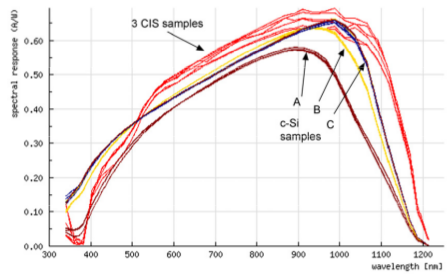
\includegraphics[scale=.5]{c-Si_SR}
\caption{Responsività spettrale di celle fotovoltaiche con silicio amorfo e monocristallino.}
\label{fig:silres1}
\end{figure}

\begin{figure}[htp]
\centering
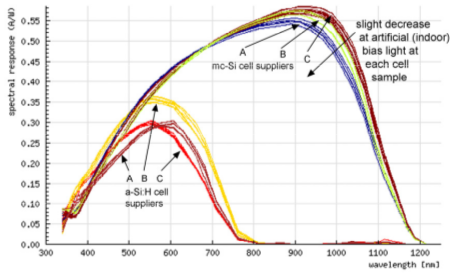
\includegraphics[scale=.5]{mc-Si_SR}
\caption{Responsività spettrale di celle fotovoltaiche con silicio multicristallino.}
\label{fig:silres2}
\end{figure}

\subsection{Hm. 2}

Fra silicio cristallino e amorfo viè una notevole differenza anche per quanto riguarda l'efficienza. In figura \ref{fig:efficiency} è riportato il confronto in termini di efficienza di varie celle fotovoltaiche con diversi tipi di silicio (amorfo, cristallino, \ldots) in funzione della luminosità in condizioni standard (STC), ovvero il flusso luminoso è limitato a 1000 lux con spettro AM1.5. Si nota come il silicio amorfo ha un'efficienza maggiore che decresce meno rapidamente a basse luminosità rispetto al silicio cristallino. Questa differenza è attribuita al fatto che il silicio amorfo possiede una resistenza si shunt naturalmente più alta.

\begin{figure}[htp]
\centering
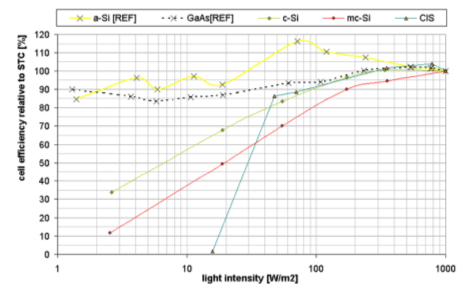
\includegraphics[scale=.5]{efficiency}
\caption{Efficienza di vari tipi di celle fotovoltaiche in funzione della luminosità incidente in \textit{Standard Test Condition}.}
\label{fig:efficiency}
\end{figure}

Infatti una cella fotovoltaica è schematizzata dal circuito equivalente in figura \ref{fig:equiv}. Pertanto una resistenza di shunt più alta, come nel caso del silicio amorfo, fa sì che una percentuale maggiore della fotocorrente generata (nello schema quella erogata dal generatore di corrente) passi nel circuito di carico e non rimanga nella fotocellula. Di fatti una delle caratteristiche per cui una cella fotovoltaica è considerata ideale è proprio a resistenza di shunt infinita.

\begin{figure}[htp]
\centering
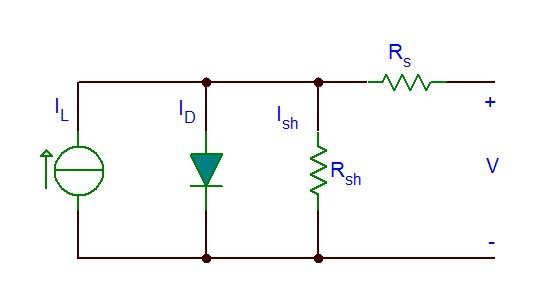
\includegraphics[scale=.5]{model}
\caption{Circuito equivalente di una cella fotovoltaica.}
\label{fig:equiv}
\end{figure}

Il modello si Shockley insieme alla conservazione della carica forniscono il seguente sistema di equazioni per la descrizione del circuito:

\begin{equation}
I_D = I_0 \, \Bigl(e^{\frac{q(V-IR_s)}{kT}}-1\Bigr)
\end{equation}

\begin{equation}
I = I_L - I_D - \frac{V-IR_s}{R_{sh}}
\end{equation}

\section{Misura della caratteristica I-V di una cella fotovoltaica}

Abbiamo simulato il circuito con TINA secondo lo schema in figura \ref{fig:simul}, ottenendo i grafici per le caratteristiche I-V e P-V al variare della resistena del potenziometro.

\begin{figure}[htp]
\centering
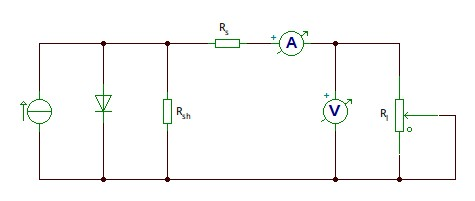
\includegraphics[scale=.4]{simul}
\caption{Circuito per la simulazione con TINA}
\label{fig:simul}
\end{figure}

In figura \ref{fig:ivchar} e \ref{fig:pvchar} sono riportati i grafici simulati, in cui si è posto $I_L = 10$ mA, $R_{sh}$ = 5 k$\Omega$, $R_s$ = 10 $\Omega$ e la resistenza è stata variata da 0 a 500 $\Omega$ (che corrisponde con il range di resistenze ottenibili con il potenziometro disponibile in laboratorio). Dalla caratteristica P-V si nota che per un certo valore della resistenza di carico si ha un massimo per la potenza erogata dalla cella. Tale resistenza la si ottiene dal rapporto $\frac{V}{I}$ alla corrispondente tensione.

\begin{figure}[htp]
\centering
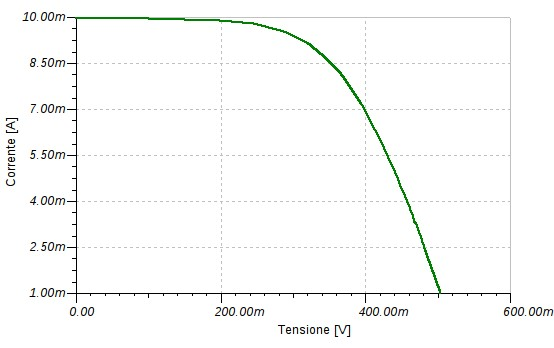
\includegraphics[scale=.4]{ivchar1}
\caption{Caratteristica I-V simulata della cella fotovoltaica}
\label{fig:ivchar}
\end{figure}

\begin{figure}[htp]
\centering
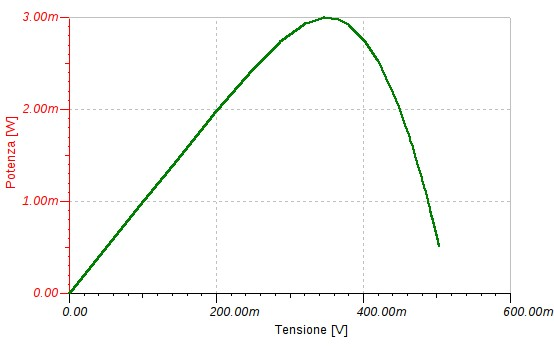
\includegraphics[scale=.4]{pvchar1}
\caption{Caratteristica P-V simulata della cella fotovoltaica}
\label{fig:pvchar}
\end{figure}

All'aumentare della resistenza di shunt i grafici precedenti non cambiano molto, dal momento che la cella fotovoltaica si avvicina al comportamento ideale, già ben approssimato con i valori precedenti. Riducend tale resistenza a 100 $\Omega$ i grafici cambiano significativamente, come si vede in figura \ref{fig:ivchar2} e \ref{fig:pvchar2}. Chiaramente la potenza massima trasferita diminuisce poichè una quantità maggiore di corrente scorre sul ramo di shunt. Aumentando $R_s$ si ottengono effetti analoghi, con una potenza massima lteriormente diminuita (meno di 1 mW) e la caratteristica I-V diventa completamente lineare.\\

\begin{figure}[htp]
\centering
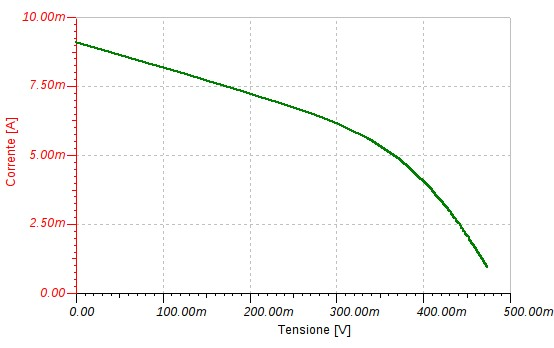
\includegraphics[scale=.4]{ivchar2}
\caption{aratteristica I-V simulata con $R_{sh}$ = 100 $\Omega$}
\label{fig:ivchar2}
\end{figure}

\begin{figure}[htp]
\centering
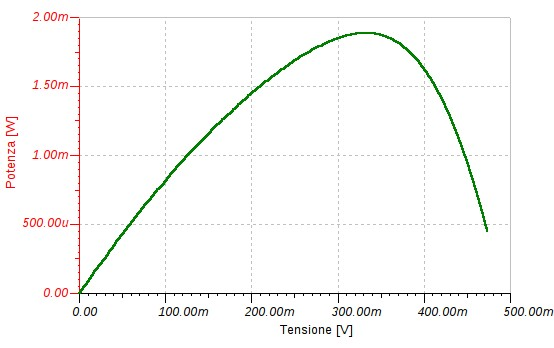
\includegraphics[scale=.4]{pvchar2}
\caption{Caratteristica P-V simulata con $R_{sh}$ = 100 $\Omega$}
\label{fig:pvchar2}
\end{figure}

Abbiamo realizzato infine sulla breadboard il circuito secondo lo schema in figura \ref{fig:mis}. Il potenziometro impiegato aveva come resistenza minima $R_{min} = 2.5(2) \Omega$ e come resistenza massima $R_{max}  = 502 \Omega \pm 0.8 \%$, abbiamo inoltre preso $R_1 = 2.5(1) \Omega$.\\

\begin{figure}[htp]
\centering
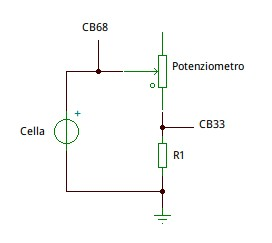
\includegraphics[scale=.6]{misura}
\caption{Schema del circuito realizzato sulla breadboard.}
\label{fig:mis}
\end{figure}

 Tramite il VI \texttt{Vin$\_$DC2ch} sono state acquisite le tensioni alla CB33 e CB68, la prima, nota $R_1$, fornisce la corrente che scorre nel circuito di carico, le seconda la tensione ai capi della cella. In tabella \ref{tab:cond} sono riportate le misure fatte con il VI in diverse condizioni.
 
\begin{table}
\centering
\caption{Valori di tensioni e correnti in varie condizioni.}
\label{tab:cond}
\begin{tabular}{|c|c|c|}
\hline 
Condizioni & Tensione (mV) & Corrente (mA) \\ 
\hline 
Luce lab & 88 & 0.205 \\ 
\hline 
Luce lab (res max) & 102 & 0.186 \\ 
\hline 
Luce lab (res min) & 2 & 0.540 \\ 
\hline 
Cella oscurata & 0 & 0.029 \\ 
\hline 
Led (res min) & 26 & 8.12 \\ 
\hline 
Led (res max) & 408 &  0.67\\ 
\hline 
Led (5 cm) & 287 & 0.488 \\ 
\hline 
Con flash (res min)& 32 & 9.81 \\ 
\hline 
\end{tabular} 
\end{table}

Come si vede da queste prime misure il comportamento della cella non contraddice l'andamento previsto, in particolare le misure fatte variando la resistenza del potenziometro.\\

Tramite il VI \texttt{Potenza$\_$celle} abbiamo tracciato la caratteristica I-V e P-V campionando le tensioni alle porte analogiche variando progressivamente la resistenza dell'amperometro. In figura \ref{fig:lab} sono mostrate le curve caratteristiche della cella alla luce ambientale. Come si vede  l'andamento ottenuto non coincide con quello in figura \ref{fig:ivchar}, ma è più lineare. A livello di simulazione con TINA si è verificato che nelle stesse condizioni, abbassando la corrente del generatore il grafico diventava sempre più lineare.

\begin{figure}[htp]
\centering
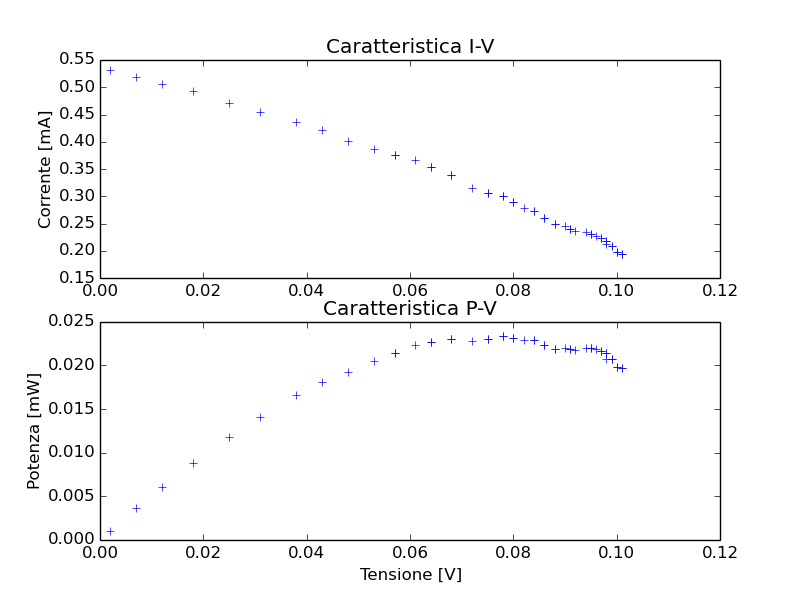
\includegraphics[scale=.45]{es4_luceamb}
\caption{Curve caratteristiche della cella alla luce del laboratorio.}
\label{fig:lab}
\end{figure}

Abbiamo fatto la stessa prova esponendo la cella alla luce di una lampada al led. Le curve ottenute si possono vedere in figura \ref{fig:led}. Questa volta il grafico è molto più simile a quello della prima simulazione, corrisponentemente alla maggiore fotocorrente generata.

\begin{figure}[htp]
\centering
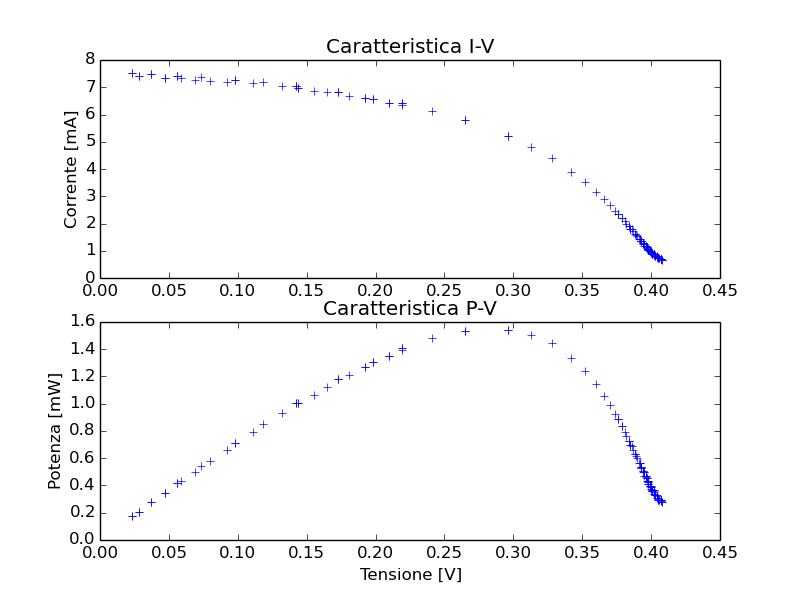
\includegraphics[scale=.45]{es4_luceled}
\caption{Curve caratteristiche della cella alla luce del laboratorio.}
\label{fig:led}
\end{figure}

Dai grafici è possibile ottenere una stima della resistenza di carico ottimale. Nel primo caso si ha che la potenza massima è erogata a V = 0.307(7) V, cui corrisponde una corrente di 0.075(3) mA, da cui la resistenza BOH
Nel secondo caso invece si ha V = 5.4(2) V e I = 0.28(1) mA, da cui R = BOH

%Lo, non tornano con quello che avevamo trovato, perché???????????????


\section{Potenza erogata in funzione dell'angolo di incidenza}

E' lecito aspettarsi una diminuzione della potenza erogata da una cella fotovoltaica all'aumentare dell'angolo di incidenza, misurato rispetto la normale alla superficie. In prima approssimazione si può pensare che la potenza incidente della radiaizone luminosa vari come il coseno dell'angolo, ciò implica una andamento analogo per la potenza erogata dato che è proporzionale a quella incidente.\\
Per verificare tali ipotesi abbiamo fatto in modo di variare l'angolo di incidenza della luce emessa da una torcia, mantenendo costante (il più possibile) la distanza fra questa e la cella fotovoltaica. Durante le acquisizioni, la cella e la torcia sono state coperte da un cartone per ridurre al minimo l'influenza dell'illuminazione ambientale. Bisogna ovviamente notare che l'approssimazione "distanza costante" non è del tutto vera, poichè le dimensioni del sistema e del pannello sono confrontabili fra di loro, quindi ad esempio, variando l'inclinazione, la porzione di superficie superiore poteva trovarsi ad una distanza dalla fonte luminosa anche il doppio rispetto alla porzione inferiore, e quindi la radiazione che giungeva sulla prima era già attenuata. Oltre a questo, anche la torcia stessa non assomiglia per nulla ad una sorgente puntiforme di radiazione, dato che è composta di un certo numero di LED dispersi spazialmente su di una superficie piuttosto ampia, a cui è anche interposta una lente.\\
Con questi caveat procediamo nelle misurazioni, stimando anche l'angolo minimo per il quale la cella è ancora capace di erogare potenza.\\

Riportiamo, per i diversi angoli di inclinazione, i grafici della corrente (asse a sx, in rosso) e della potenza (asse a dx, in blu) in funzione della tensione fornita dalla CB68.
\textbf{Attenzione}: nei seguenti grafici gli angoli sono rispetto all'orizzontale. Con l'ovvia trasformazione $\theta \rightarrow 90 - \theta$ si ottengono i gradi rispetto alla normale.

\begin{figure}
\centering
\subfloat[Subfigure 1 list of figures text][Subfigure 1 caption]{
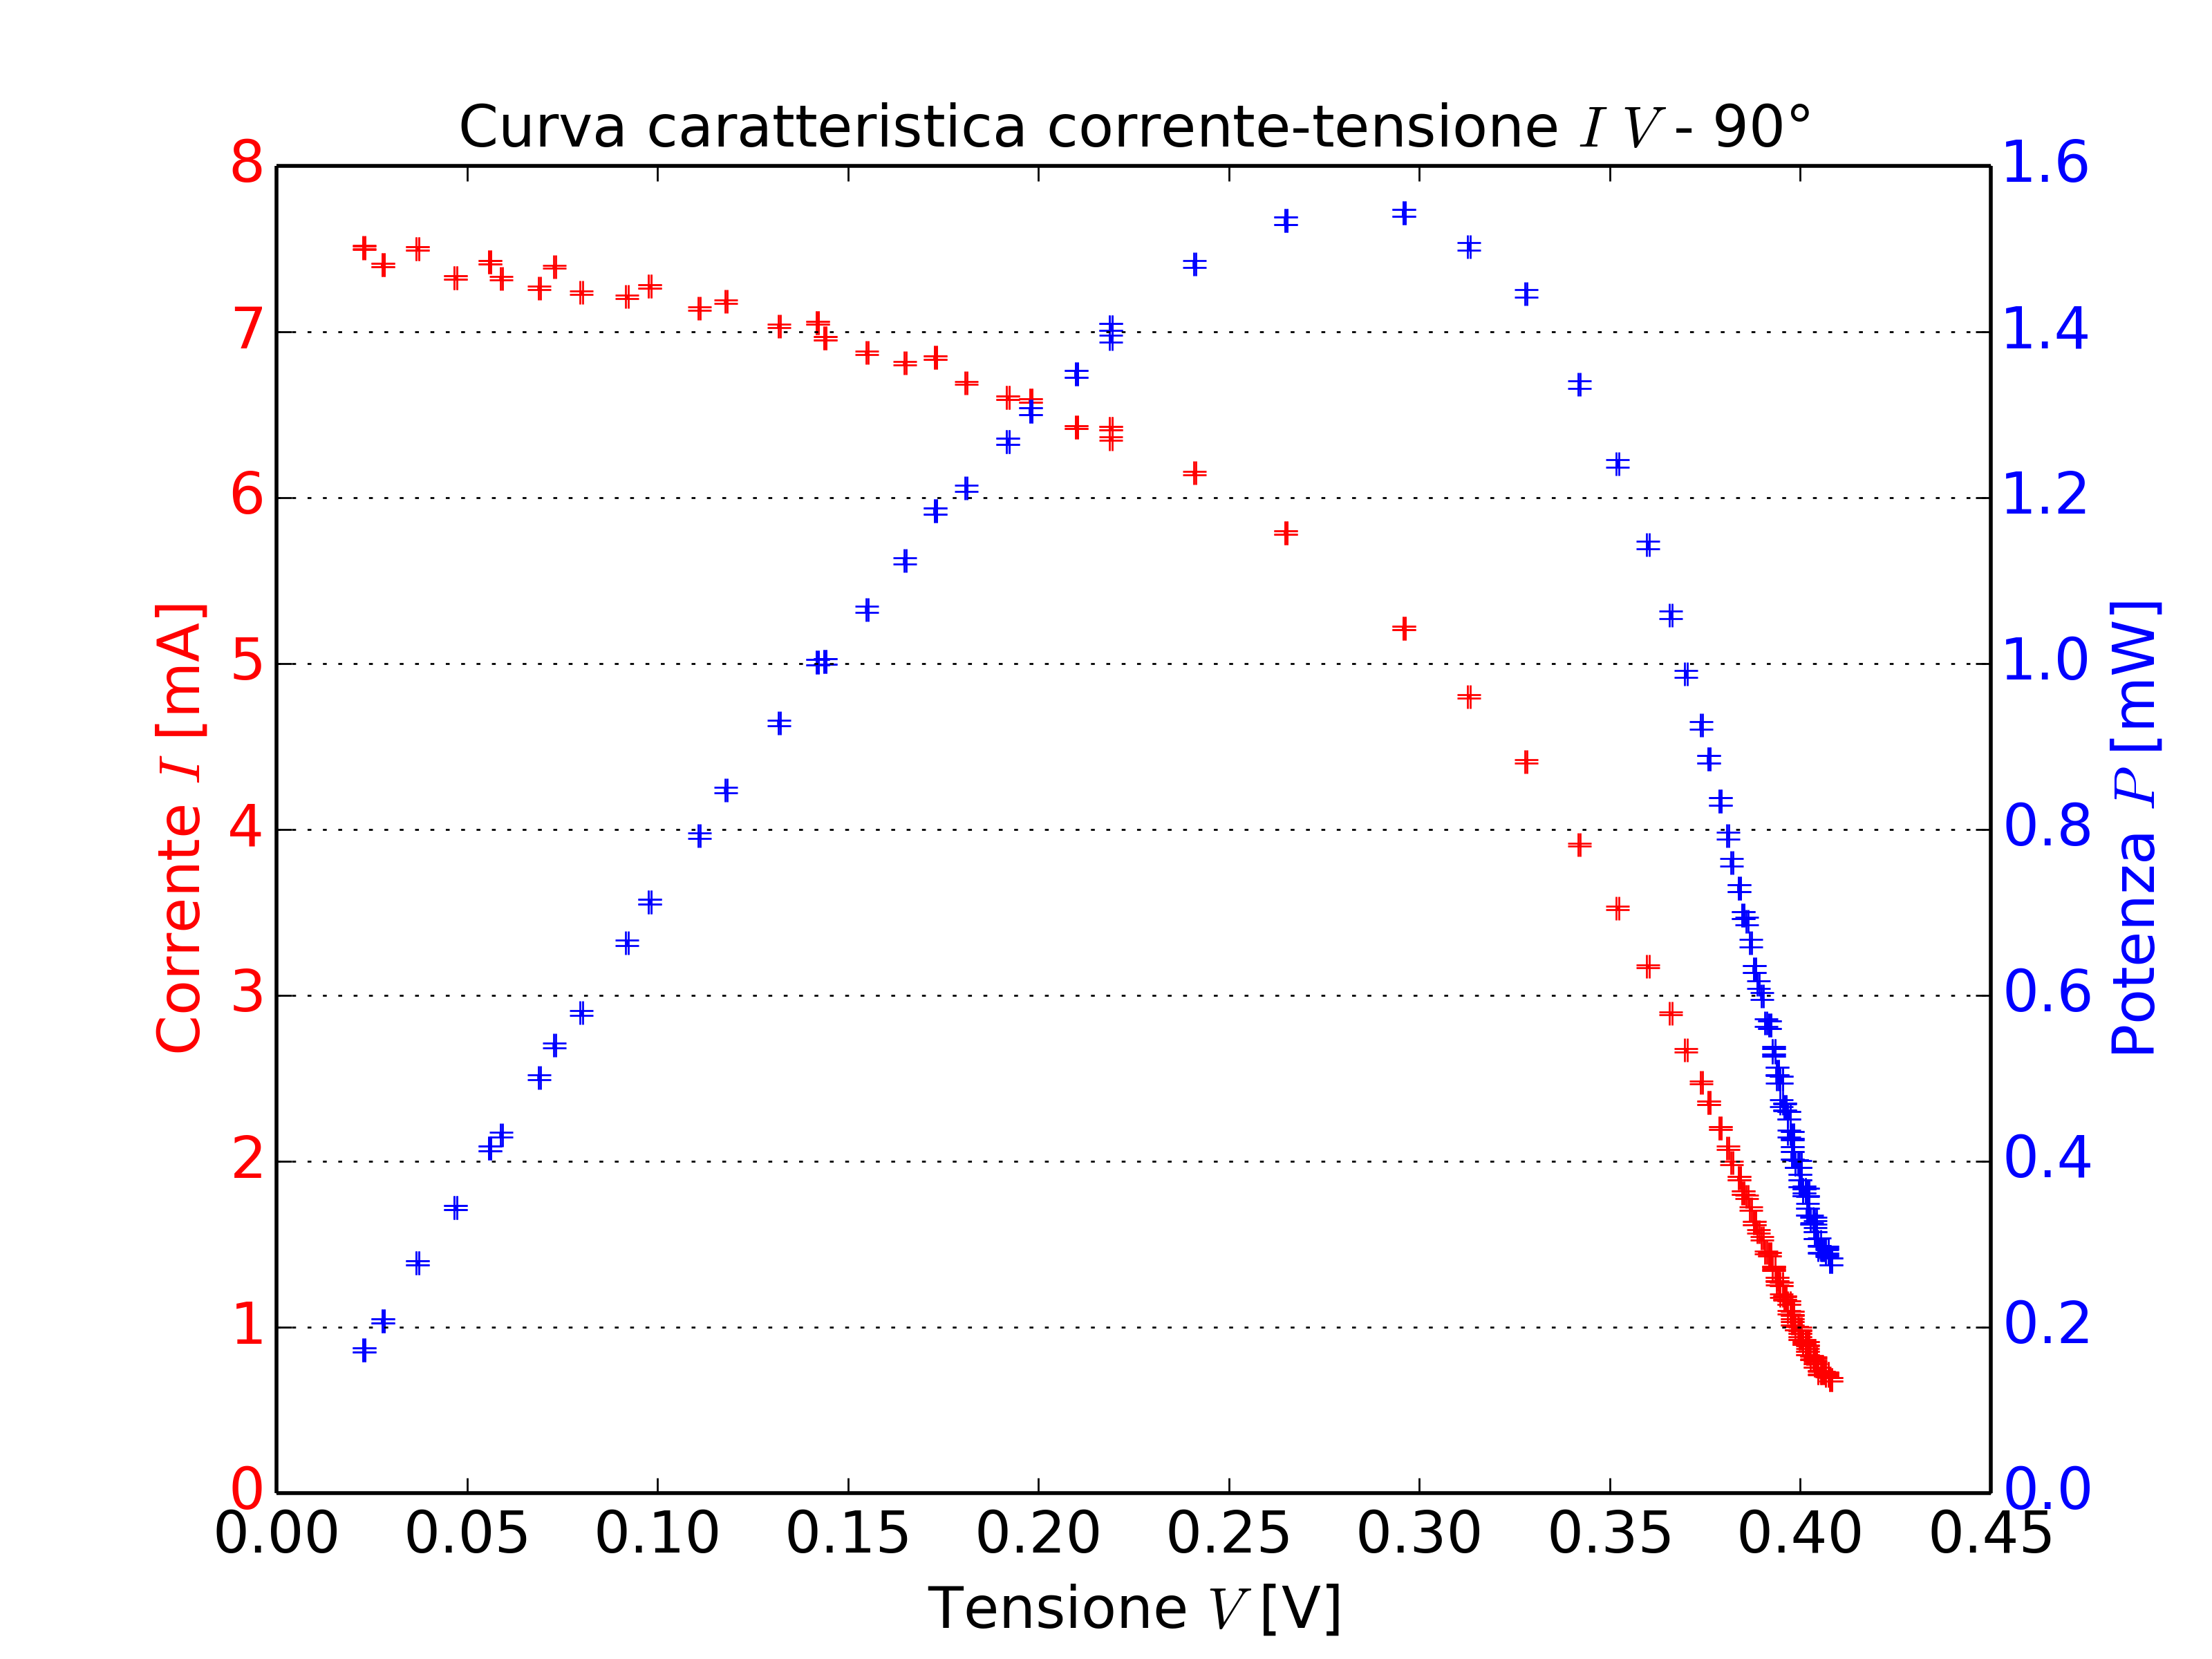
\includegraphics[width=0.9\linewidth]{./es6_ref}
\label{fig:subfig1}}
\qquad
\subfloat[Subfigure 2 list of figures text][Subfigure 2 caption]{
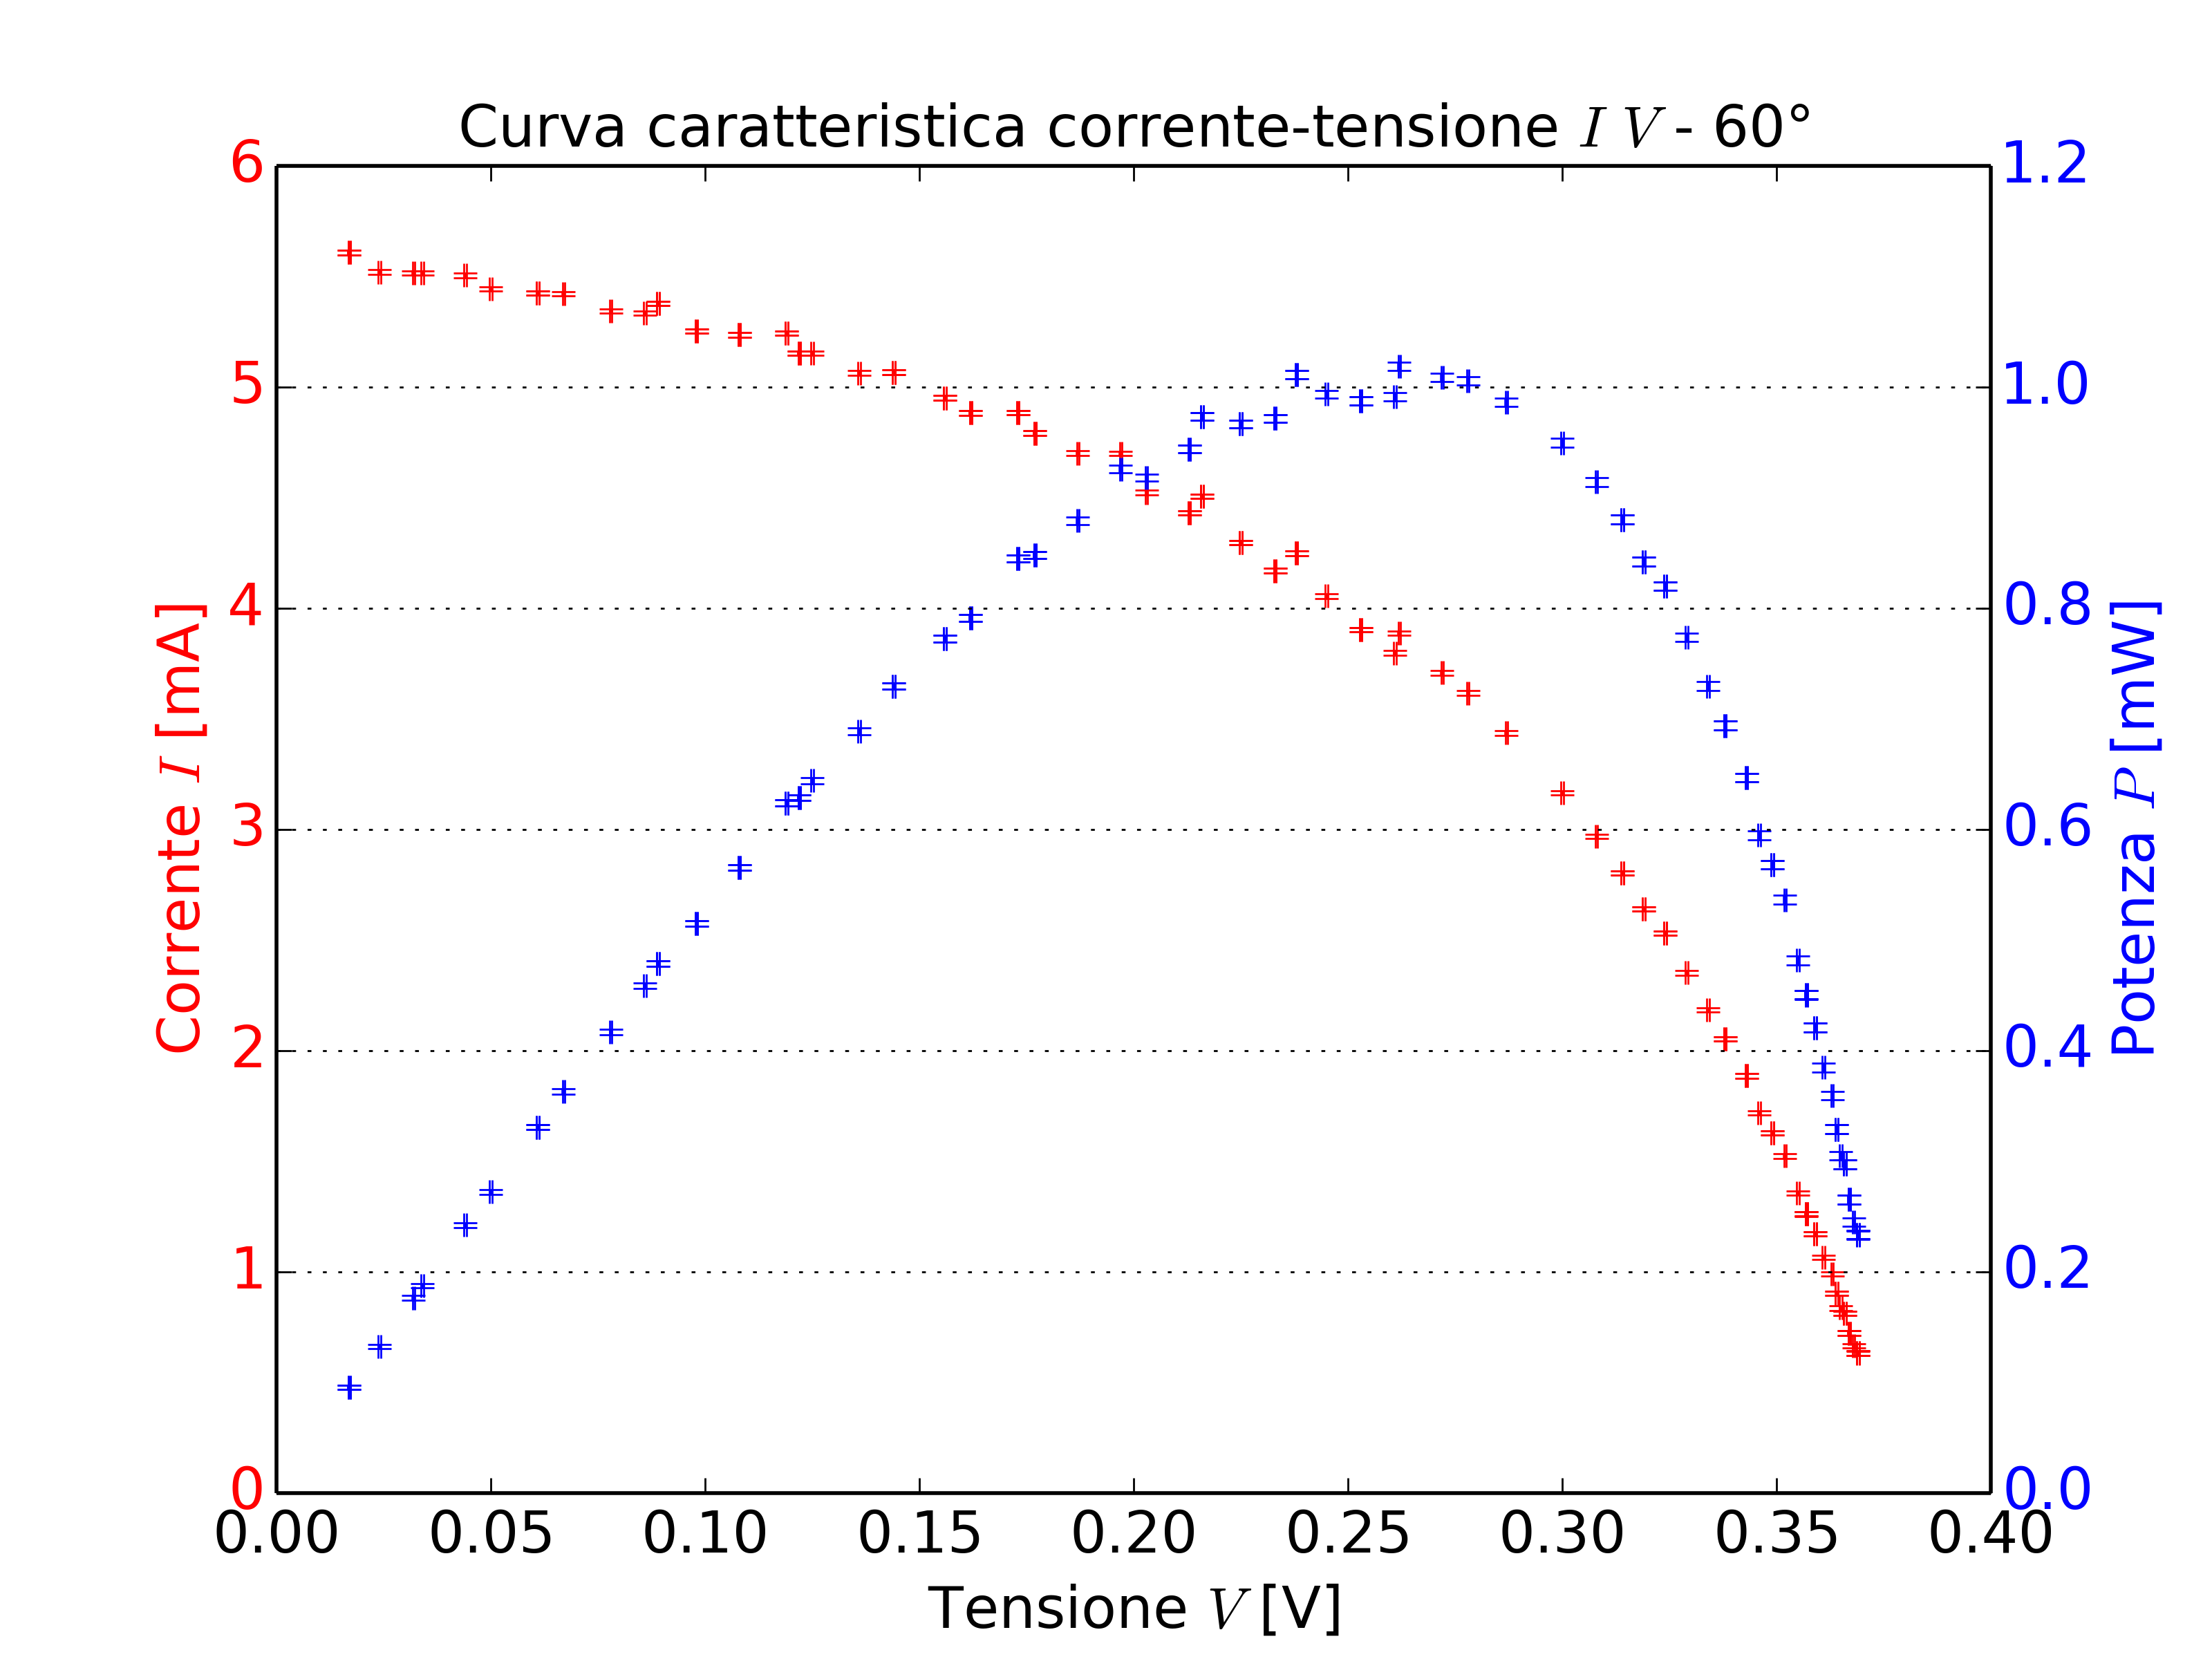
\includegraphics[width=0.9\linewidth]{./es6_60}
\label{fig:subfig2}}
\qquad

\caption{This is a figure containing several subfigures.}
\label{fig:globfi6}
\end{figure}

\begin{figure}
\centering
\subfloat[Subfigure 3 list of figures text][Subfigure 3 caption]{
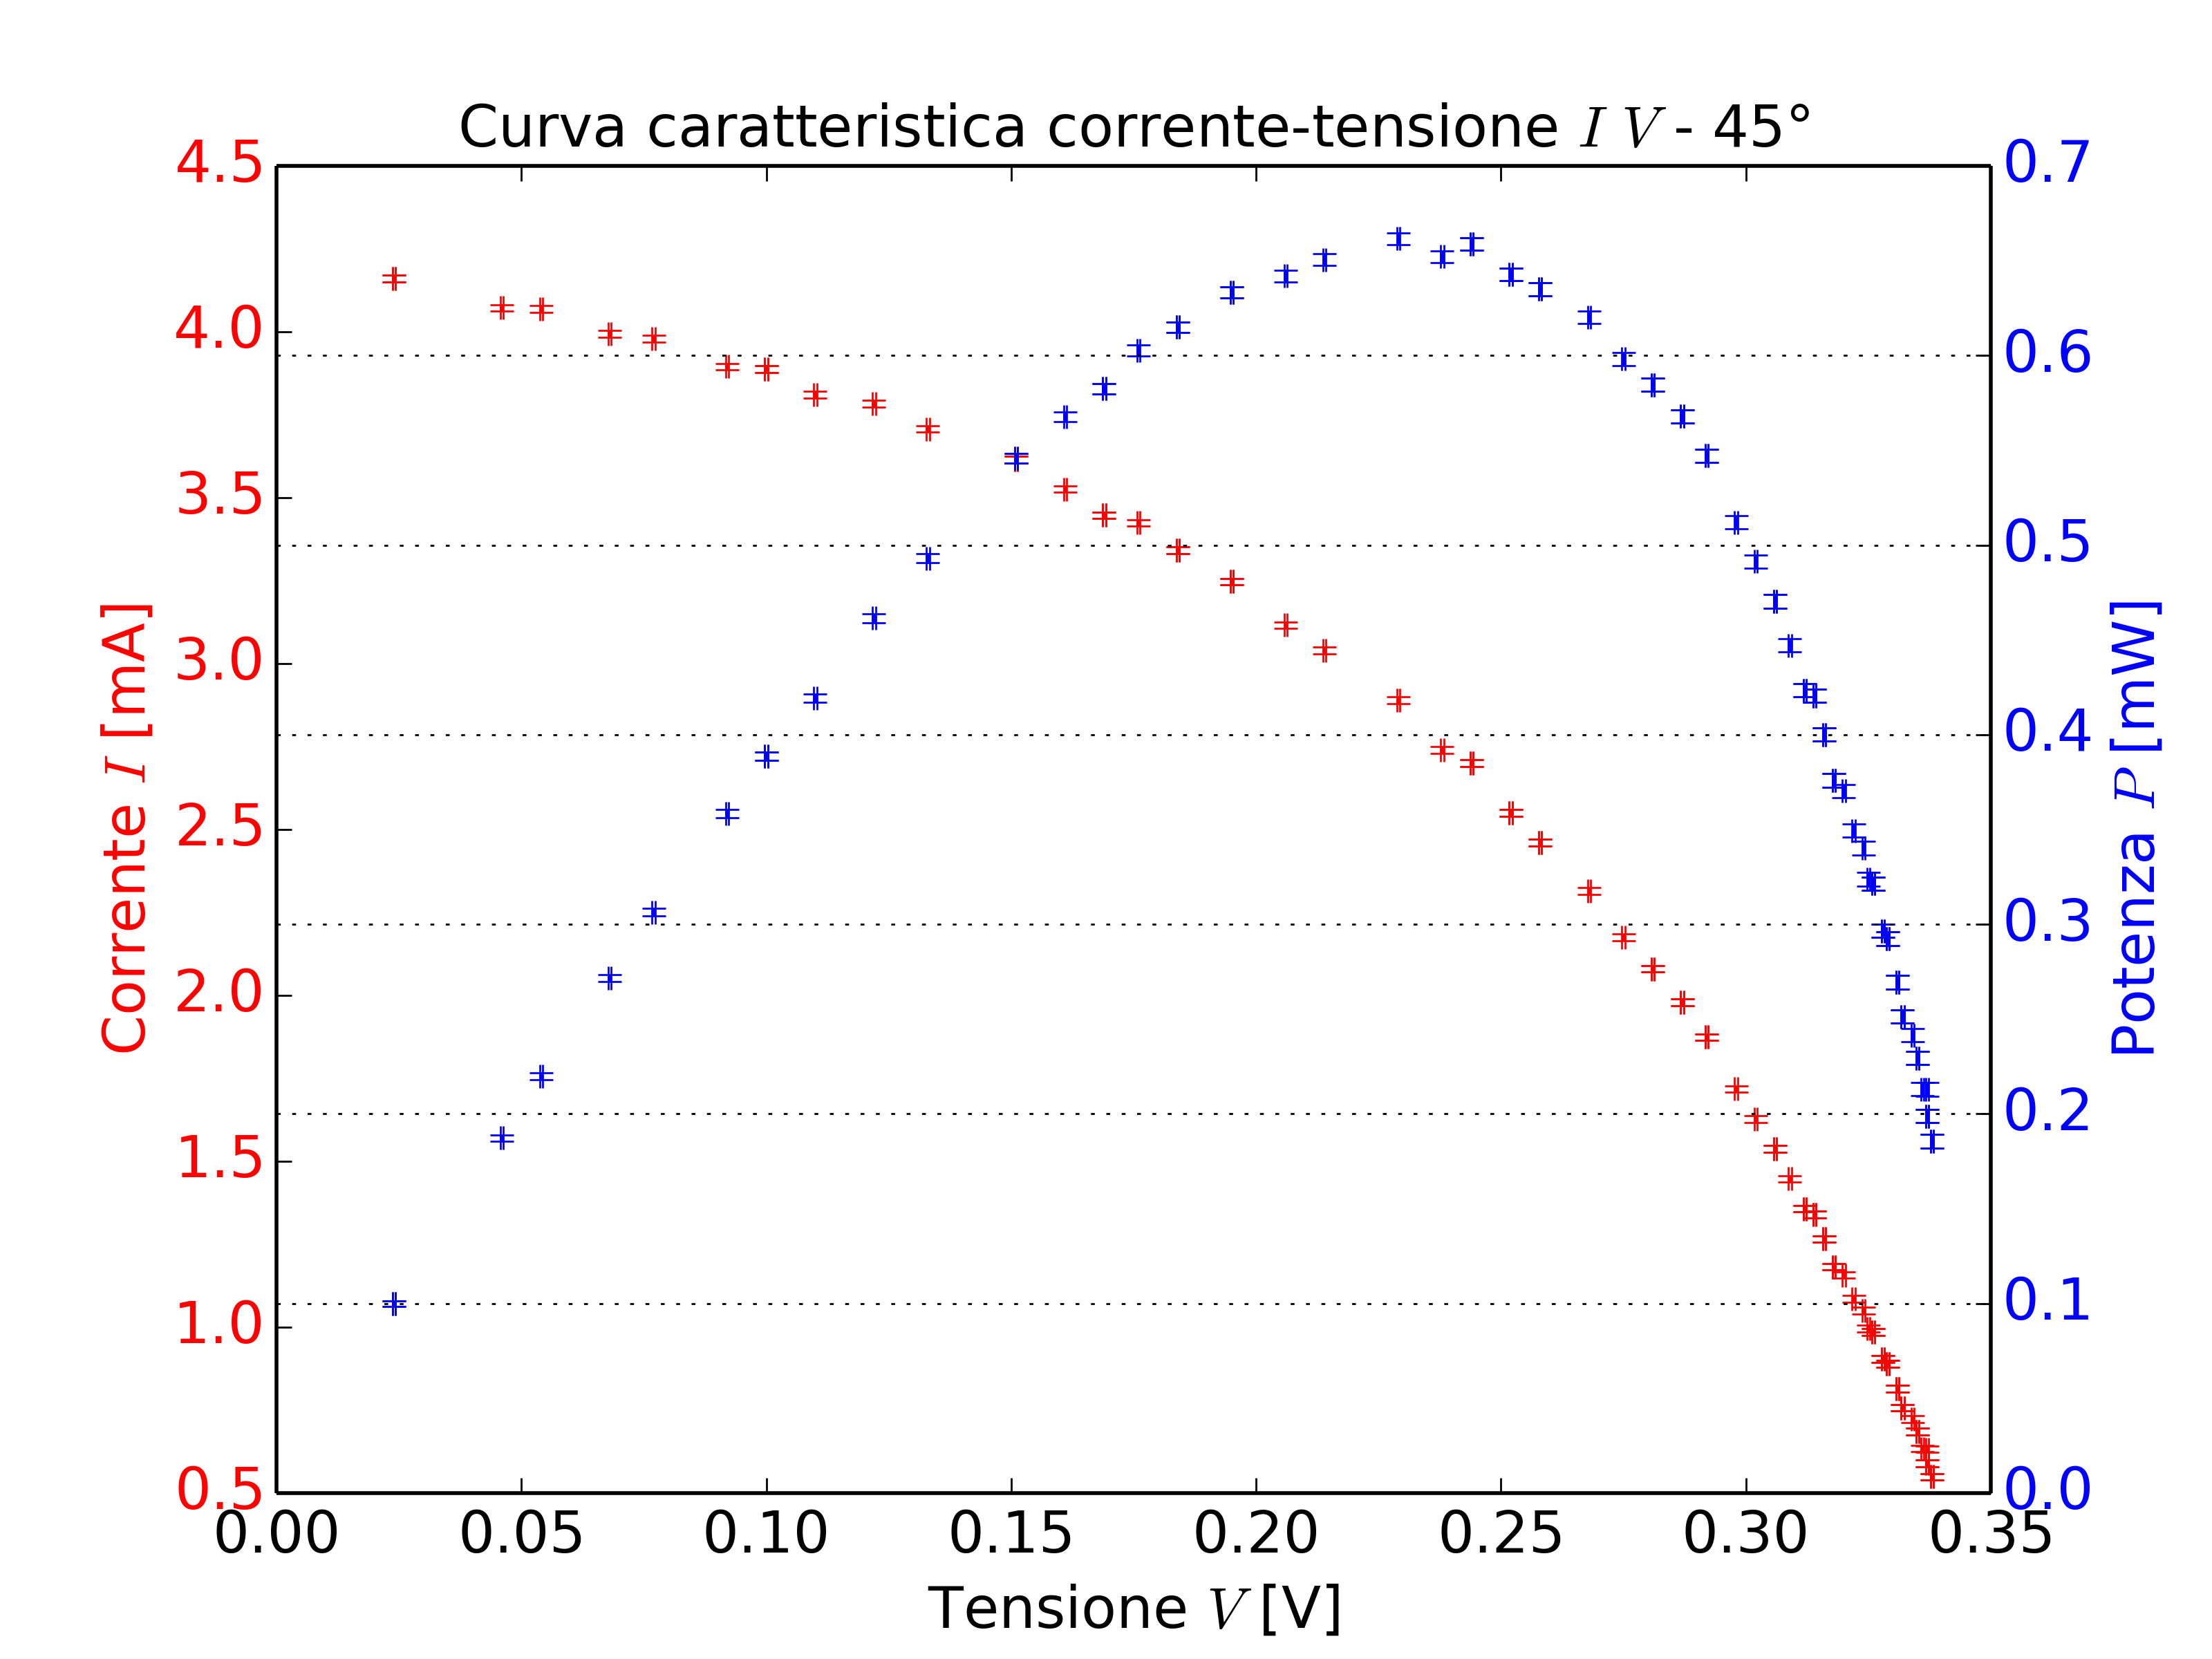
\includegraphics[width=0.9\linewidth]{./es6_45}
\label{fig:subfig3}}
\qquad
\subfloat[Subfigure 4 list of figures text][Subfigure 4 caption]{
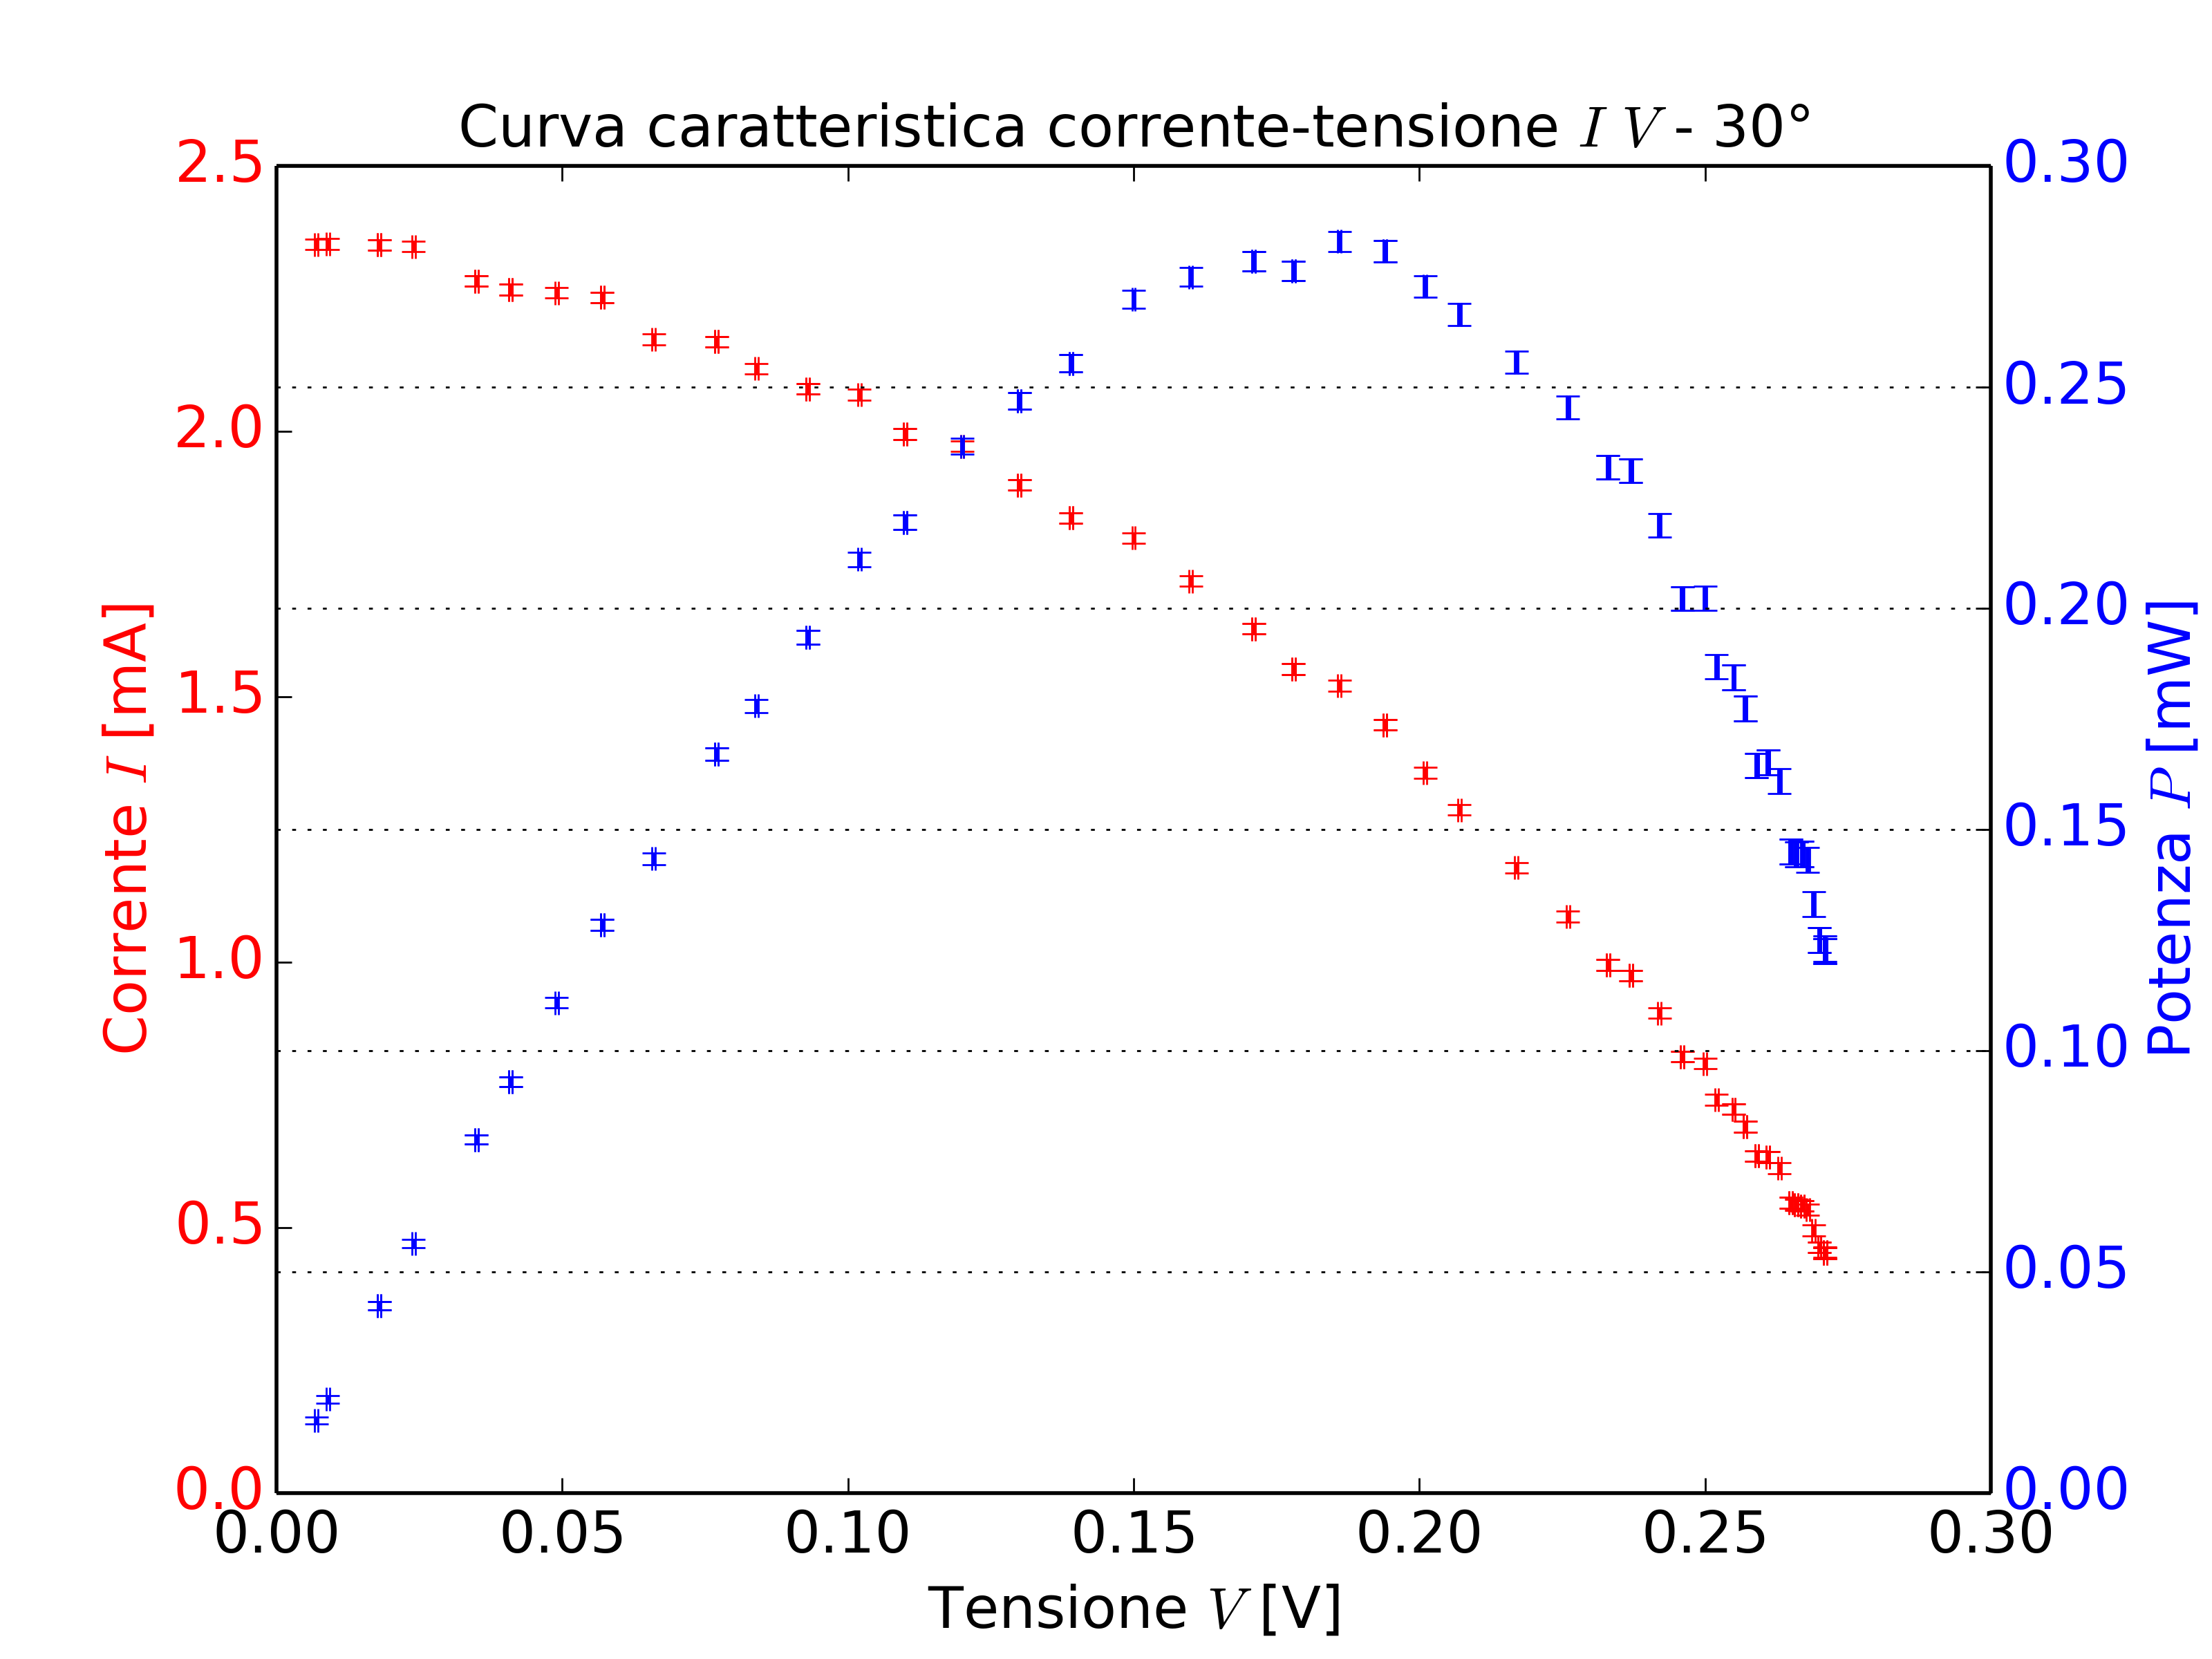
\includegraphics[width=0.9\linewidth]{./es6_30}
\label{fig:subfig4}}
\caption{This is a figure containing several subfigures.}
\label{fig:globfiy}
\end{figure}

\begin{figure}
\centering
\subfloat[Subfigure 4 list of figures text][Subfigure 4 caption]{
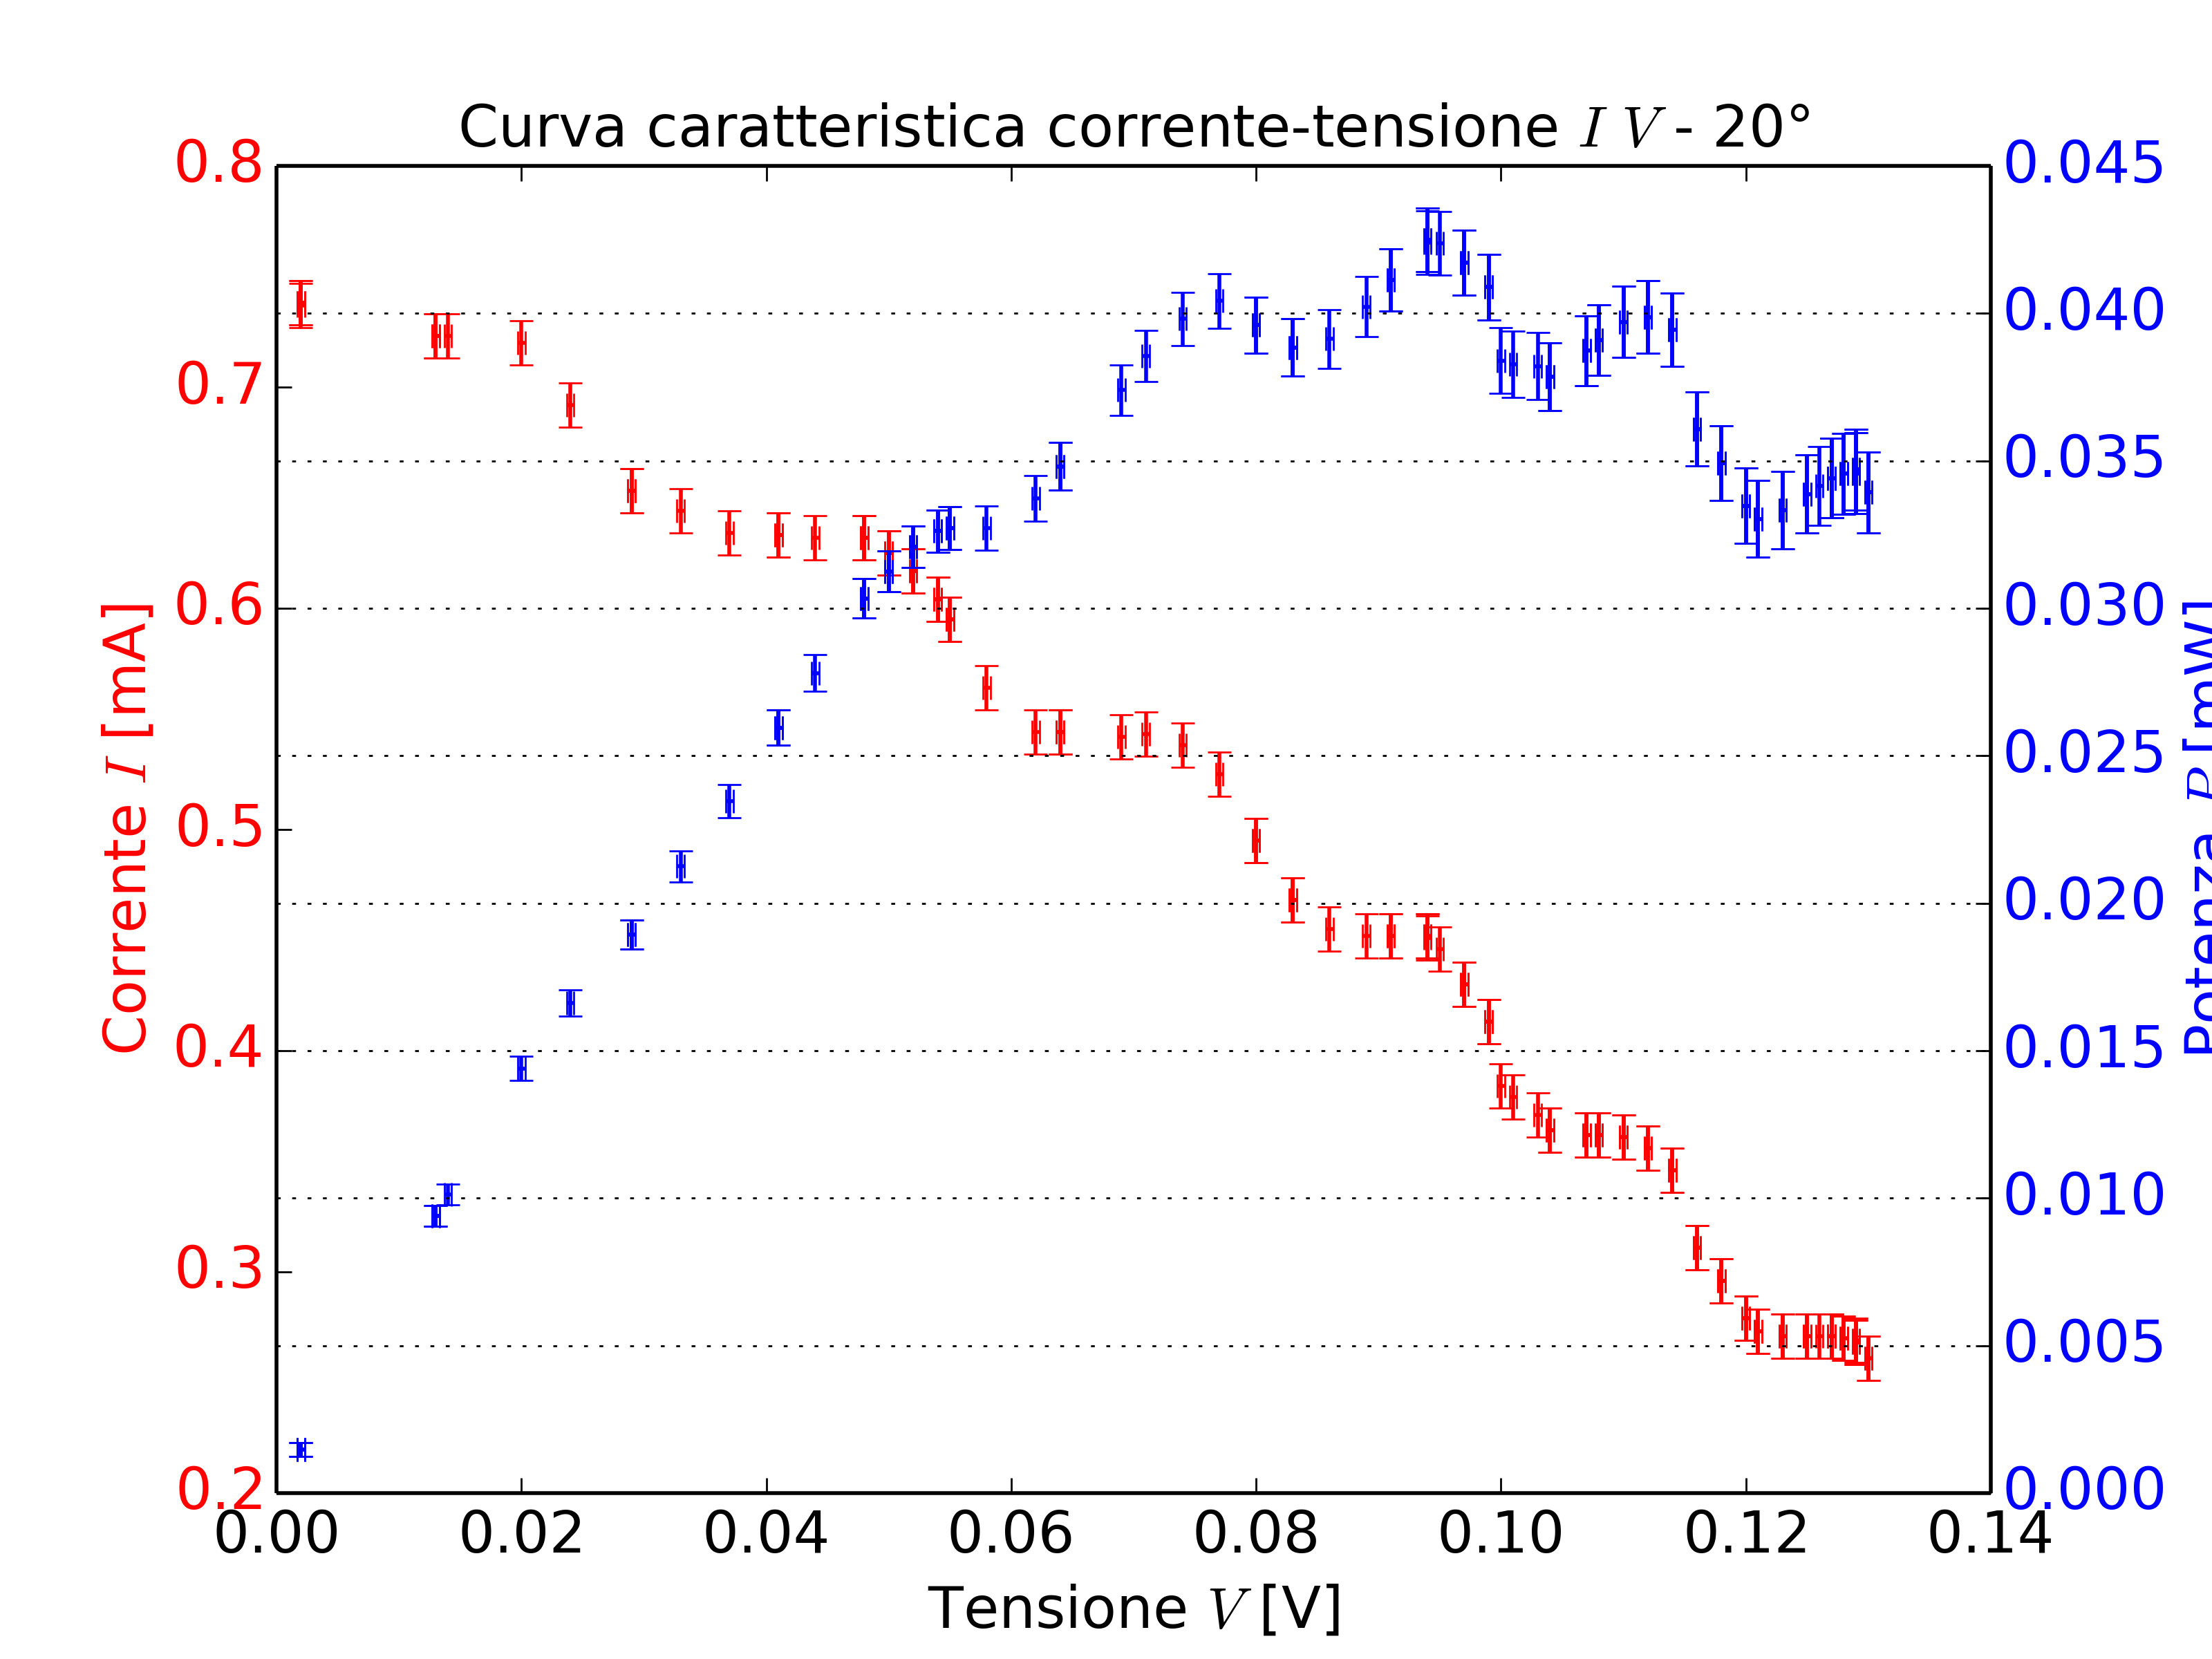
\includegraphics[width=0.9\linewidth]{./es6_20}
\label{fig:subfig5}}
\qquad
\subfloat[Subfigure 4 list of figures text][Subfigure 4 caption]{
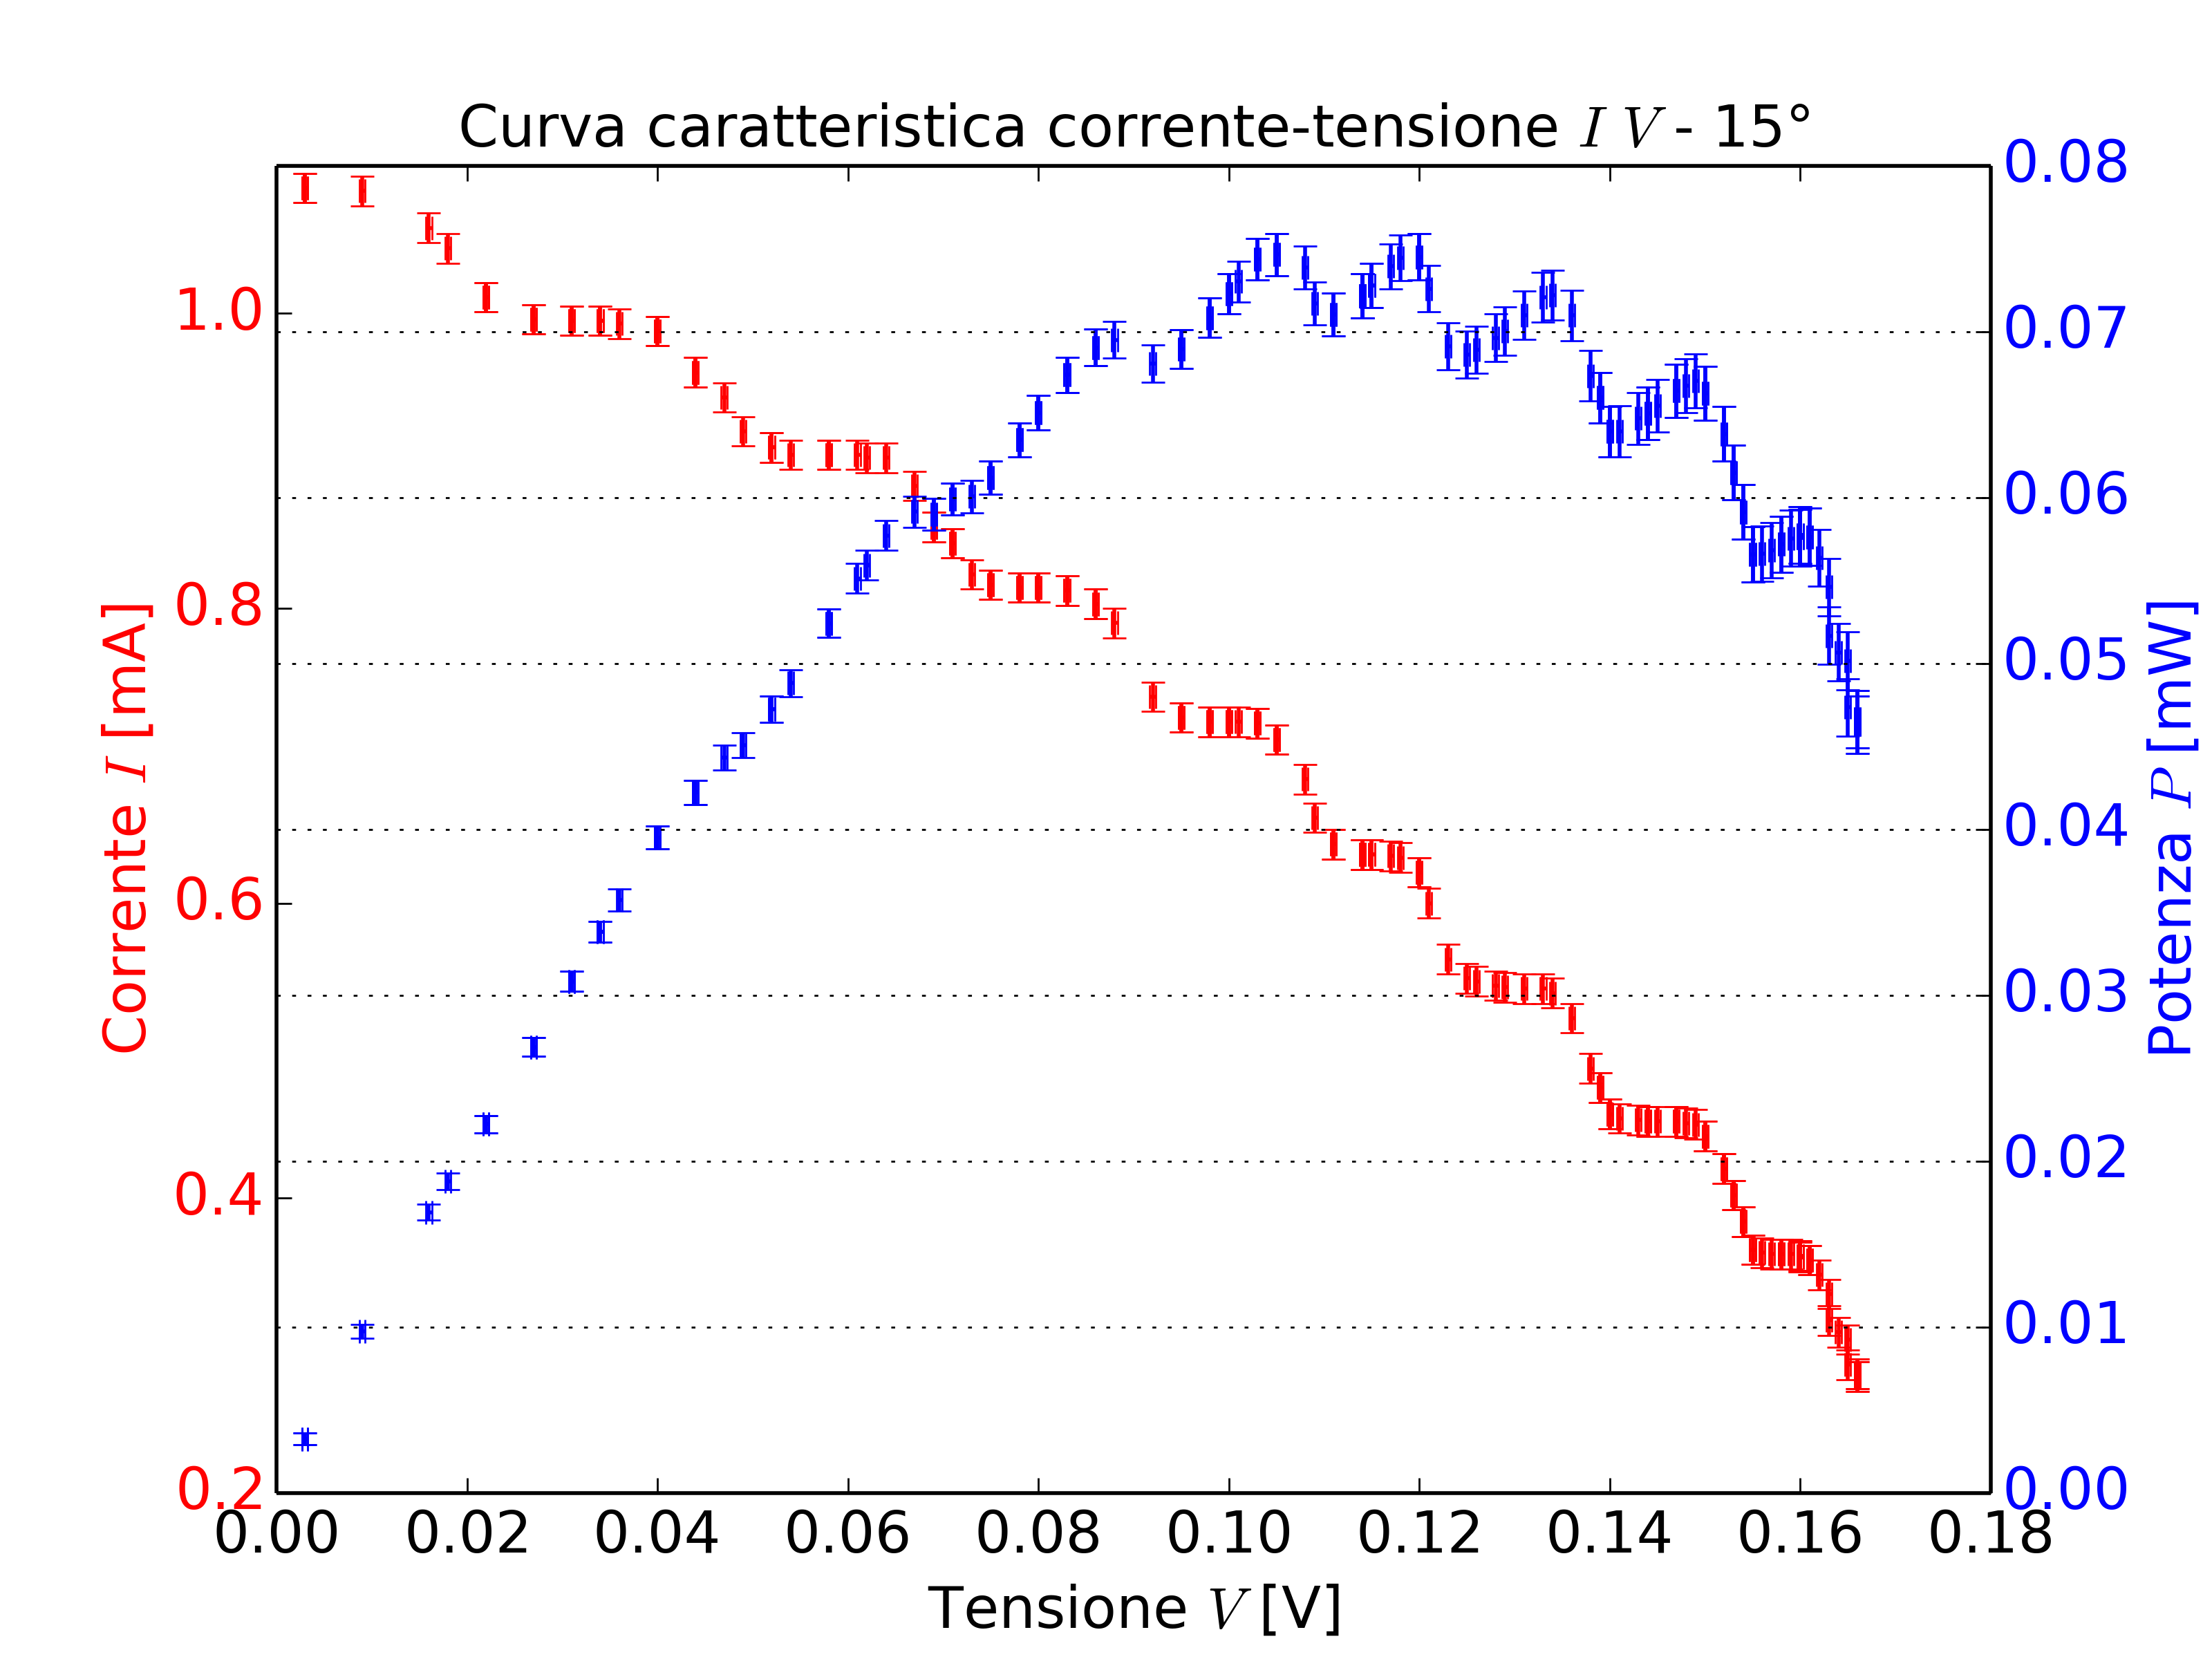
\includegraphics[width=0.9\linewidth]{./es6_15}
\label{fig:subfig6}}
\caption{This is a figure containing several subfigures.}
\label{fig:globfi3}
\end{figure}

Notiamo in particolare, nelle curve riferite agli angoli di 20\textdegree e 30\textdegree (rispetto all'orizzontale), dei curiosi andamenti "a scalini" della corrente in funzione della tensione. Diverse prove hanno mostrato che questo fenomeno appare visibile per correnti uguali o inferiori ad 1mA. Inoltre, ogni scalino sembra portare ad un dislivello costante di un decimo di mA lungo lo stesso grafico e anche nei grafici con inclinazioni diverse. \\
La prima spiegazione che abbiamo provato a darci prende in considerazione, ovviamente, la risoluzione della scheda sulle tensioni misurate, tuttavia tramite alcuni controlli abbiamo escluso questa possibilità: in tutte le acquisizioni la risoluzione determinata dal fondoscala è sensibilmente minore del dislivello. Ciò è evidente anche dal fatto che non vi sono discontinuità, ma la discesa è continua con dei campionamenti intermedi.\\
Tale andamento non sembra neppure dipendere sostanzialmente dall'angolo di incidenza: si intuisce qualcosa di analogo anche a 30 \textdegree e probabilmente si potrebbe osservare anche per angoli superiori se la strumentazione ci avesse permesso di esplorare regioni di basse correnti con sufficiente risoluzione.\\
Una seconda ipotesi, supponendo che questo fenomeno dipenda da processi macroscopici e non quantistici, lega questo andamento a dei fattori costruttivi della cella stessa, che è a sua volta composta da un grande numero di giunzioni collegate fra loro in un certo modo e, probabilmente, raggruppate in sub-celle. A questo punto potrebbe entrare in gioco una qualche forma di "attivazione" sequenziale di resistenze in parallelo di tutte le giunzioni in base al variare della resistenza esterna di carico, che potrebbe spiegare (dato il piccolo valore delle singola resistenza del gruppo di giunzioni) per quale motivo questo comportamento risulti evidente a basse correnti.\\

Per avere un'idea un po' più chiara per la variazione della potenza erogata in funzione dell'inclinazione (rispetto, questa volta, alla \textbf{normale}), si riporta in Figura (\ref{fig:es6_angles_plot}) un grafico in cui vi sono i valori massimi della potenza per ogni rilevazione mostrata in precedenza. L'andamento è quello previsto, anche se i dati non sono sufficienti per verificare una certa dioendenza funzionale rispetto ad un'altra, tuttavia stranamente il dato della potenza massima $P_{max}$ riferito ai 15\textdegree risulta maggiore di quello dei 20\textdegree. Probabilmente ciò è dovuto al fatto che, come già spiegato, le approssimazioni di distanza costante non sono ben verificate, e specialmente a questi angoli, oltre che ad una generale bassa accuratezza delle stime delle inclinazioni, dato l'apparato sperimentale molto "artigianale".\\

\begin{figure}
\centering
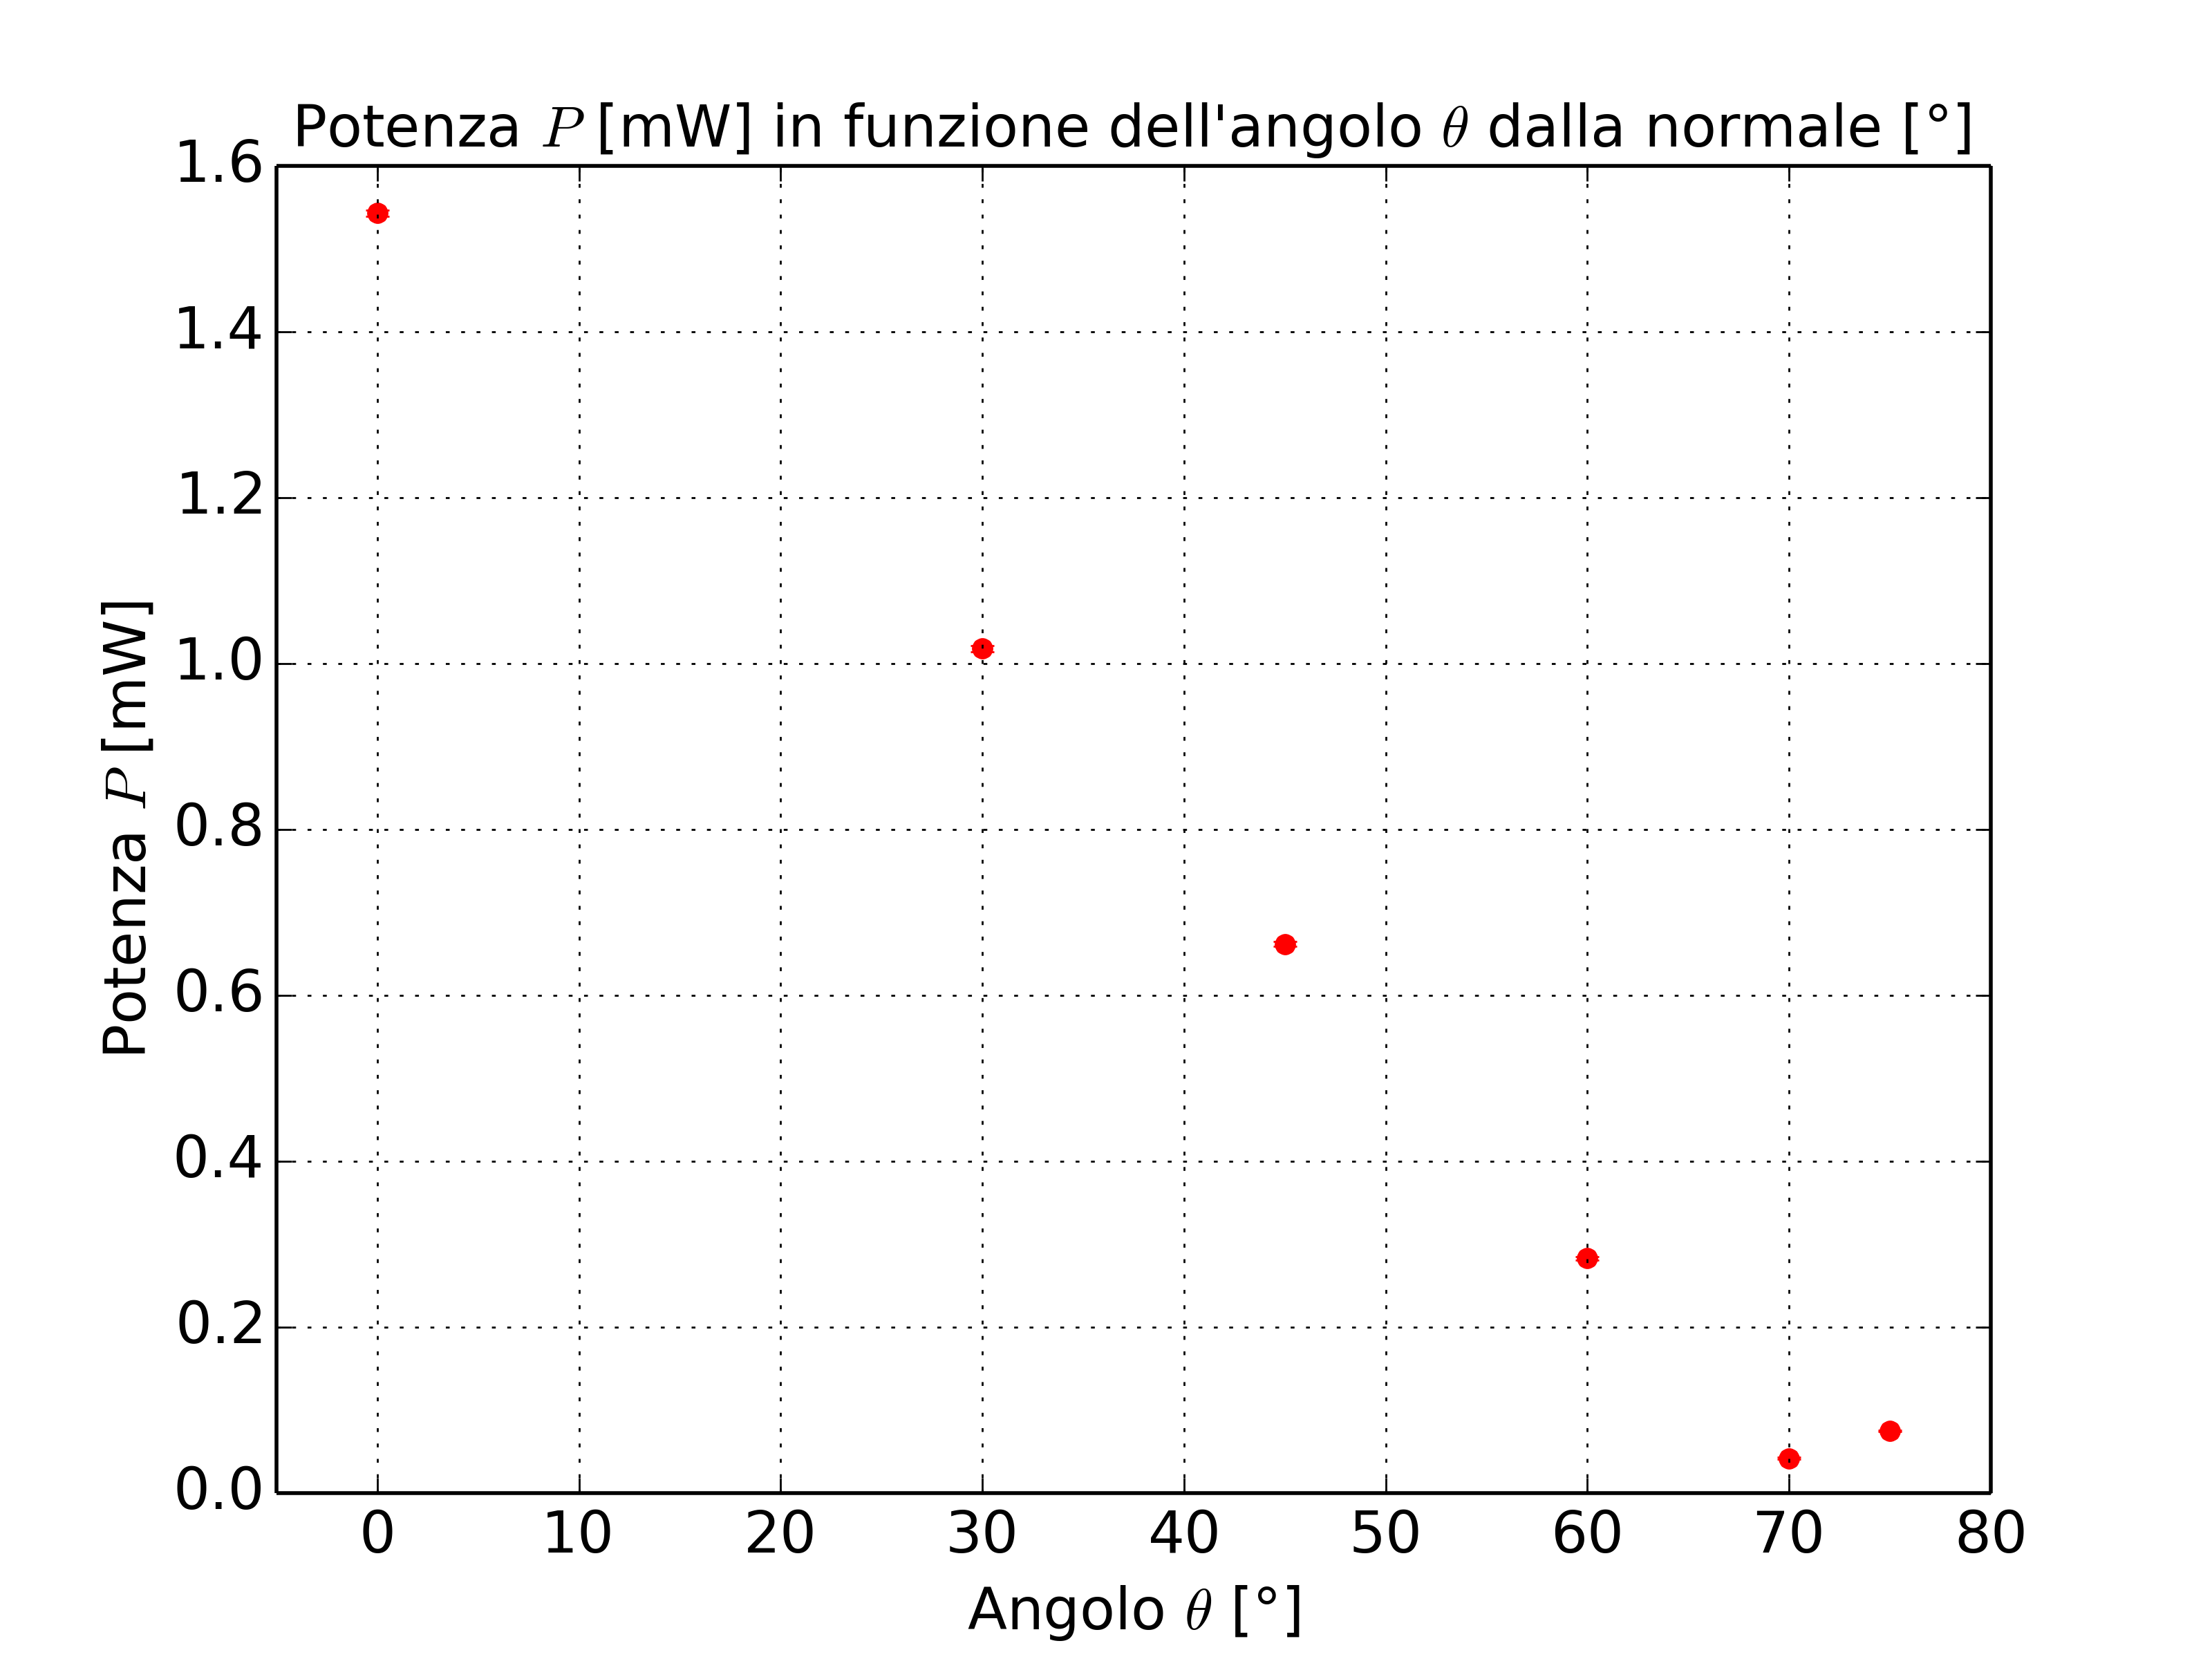
\includegraphics[width=0.9\linewidth]{./es6_angles_plot}
\caption{Potenza massima in funzione dell'angolo di incidenza della radiazione rispetto alla normale della superficie.}
\label{fig:es6_angles_plot}
\end{figure}

\begin{tabular}{|c|c|}
\hline Angolo (normale) [\textdegree] & Potenza max [mW] \\ 
\hline 0 & 1.543(4) \\ 
\hline 30 & 1.018(4) \\ 
\hline 45 & 0.662(3) \\ 
\hline 60 & 0.283(2) \\ 
\hline 70 & 0.042(1) \\ 
\hline 75 & 0.075(1) \\ 
\hline 
\end{tabular} 

~\\

\section{Curva caratteristica I-V al variare della distanza}
In questa sezione cerchiamo, invece, di verificare l'andamento della potenza massima con il variare della distanza della sorgente luminosa dalla cella (mantenendoci a inclinazione costante e perpendicolare alla superficie). A nostra disposizione abbiamo avuto la lampada "grande" (rispetto alla torcia usata precedentemente), e per questo motivo, oltre che per ragioni di comodità, sono state scelte distanze comprese fra i 50 e i 90 cm circa. Se la sorgente fosse puntiforme ci aspetteremmo un'andamento della potenza incidente (e quindi erogata) come $1/r^2$ (fronti d'onda sferici), ma ancor più che per la torcia, queste ipotesi non sono verificate. In generale ci aspettiamo comunque una diminuzione della potenza con l'aumentare della distanza.\\

In un unico grafico piuttosto articolato ma di facile interpretazione (Figura (\ref{fig:es7_prova})), riportiamo tutte le caratteristiche I-V per le varie distanze scelte, usando le stesse convenzioni di prima, e cioè con una scala a sx per le correnti, una a dx per la potenza. Sono evidenziati, inoltre, i punti di potenza massima e le distanze (in cm) a cui fanno riferimento le diverse curve. \\

\begin{figure}
\centering
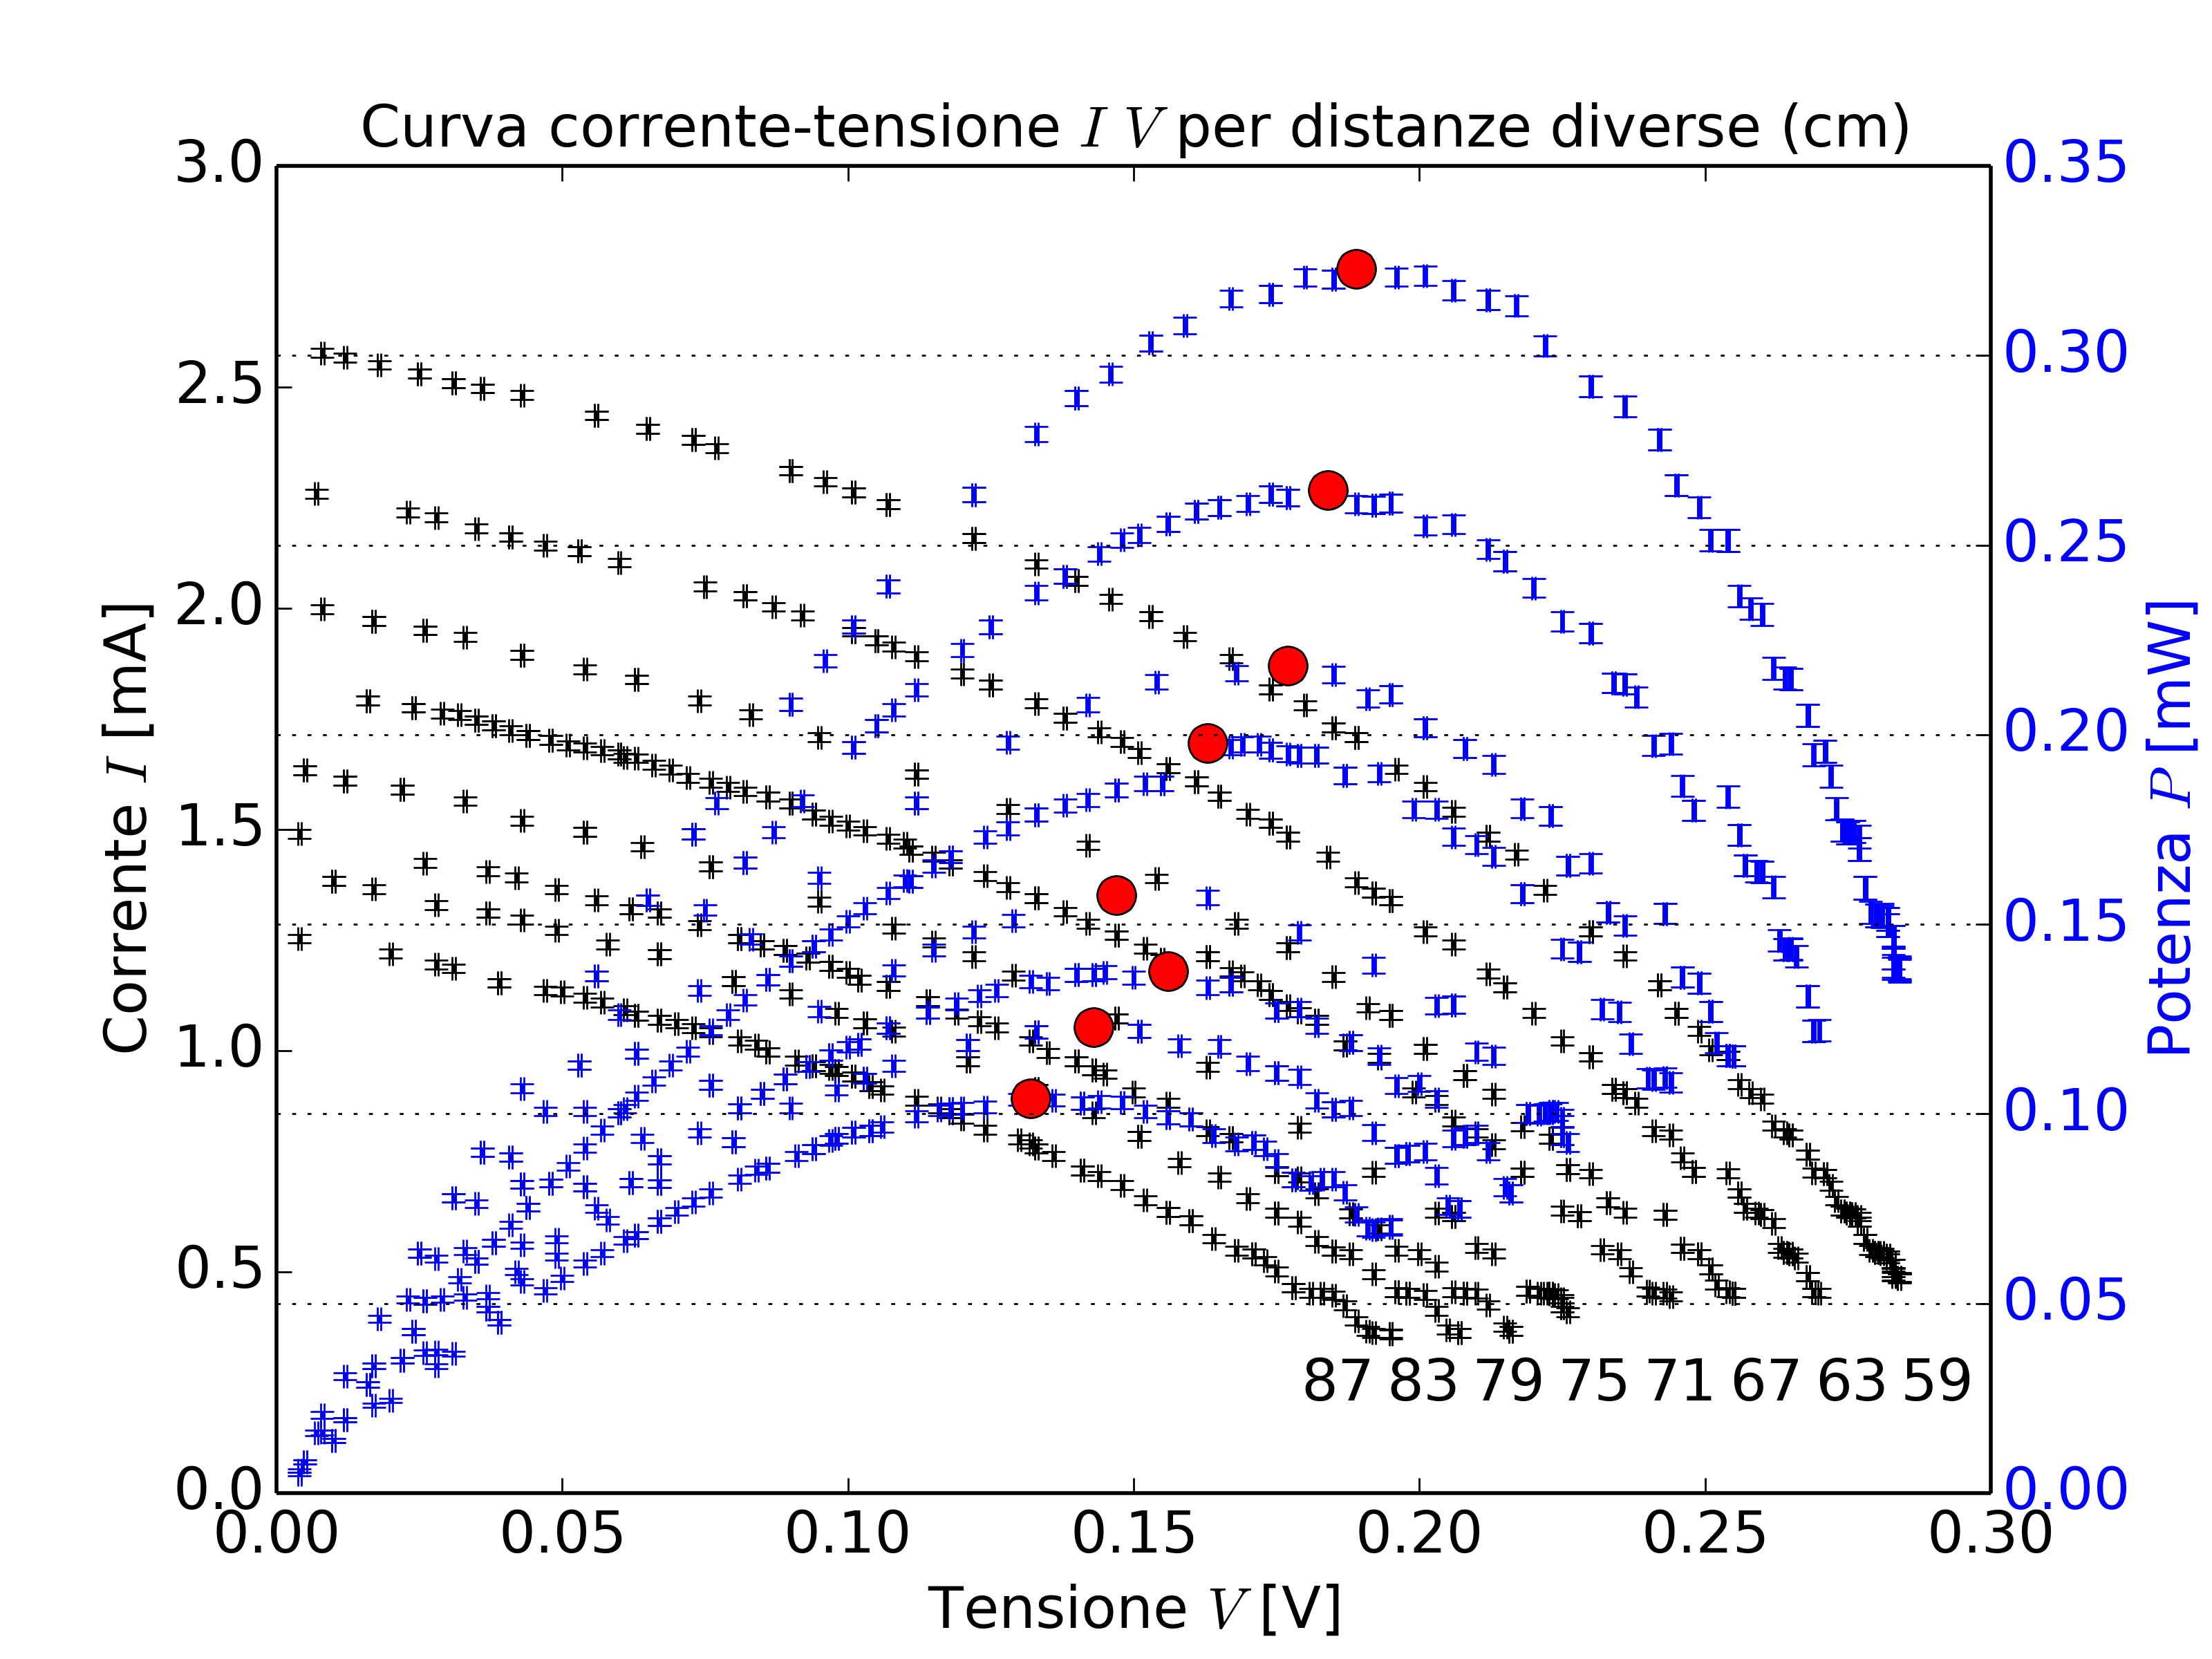
\includegraphics[width=1\linewidth]{./es7_prova}
\caption{Caratteristiche I-V e P-V della cella in funzione della distanza.}
\label{fig:es7_prova}
\end{figure}

Come si nota, sia la corrente massima $I_{max}$ (definita come la corrente per cui si ha potenza massima), sia la tensione massima $V_{max}$ (definizione analoga), tendono a diminuire con l'aumentare della distanza.\\

Proviamo a fittare i dati della potenza massima in funzione della distanza per capire di quanto si discostano (se si discostano) dall'andamento $1/r^2$ del modello semplificato.\\
In Figura(\ref{fig:es7_fit_fissexp}), si riporta il best-fit dei dati \textbf{fissato} l'esponente negativo della potenza di $r$ pari a 2. La funzione di fit usata è a due parametri:

\begin{equation}
f(x) = \frac{par[0]}{(x-par[1])^2}
\end{equation}

Il $\chi^2$ è ragionevole (si veda la figura) in base al numero di gradi di libertà. Vediamo anche che la curva di best-fit approssima piuttosto bene i dati sperimentali. Ci aspettiamo, quindi, che anche introducendo come ulteriore parametro uno scostamento dall'esponente 2, questo debba essere piuttosto piccolo. Riportiamo, quindi, in Figura (\ref{fig:es7_fit_devexp}) il fit con esponente \textbf{libero}. Si ottiene uno scostamento dalla potenza 2 minore di 1 (circa 0.88) e soprattutto compatibile con zero. Osserviamo, però, che nelle scale impiegate in base ai dati acquisiti, una curva con potenza di x pari a 2, o pari a 2.88, sono molto vicine fra loro. \\
La conclusione che traiamo è che se avessimo avuto qualche misura della potenza a distanze di 20 o 30 cm il fit avrebbe potuto discriminare molto meglio fra le due potenze, poichè queste per x piccoli sono ben distinguibili. In altre parole: la radice cubica e la radice quadrata, per argomenti (la potenza nel nostro caso) minori di 1 sono vicine fra loro, per argomenti maggiori di 1 sono molto distanti.

\begin{figure}
\centering
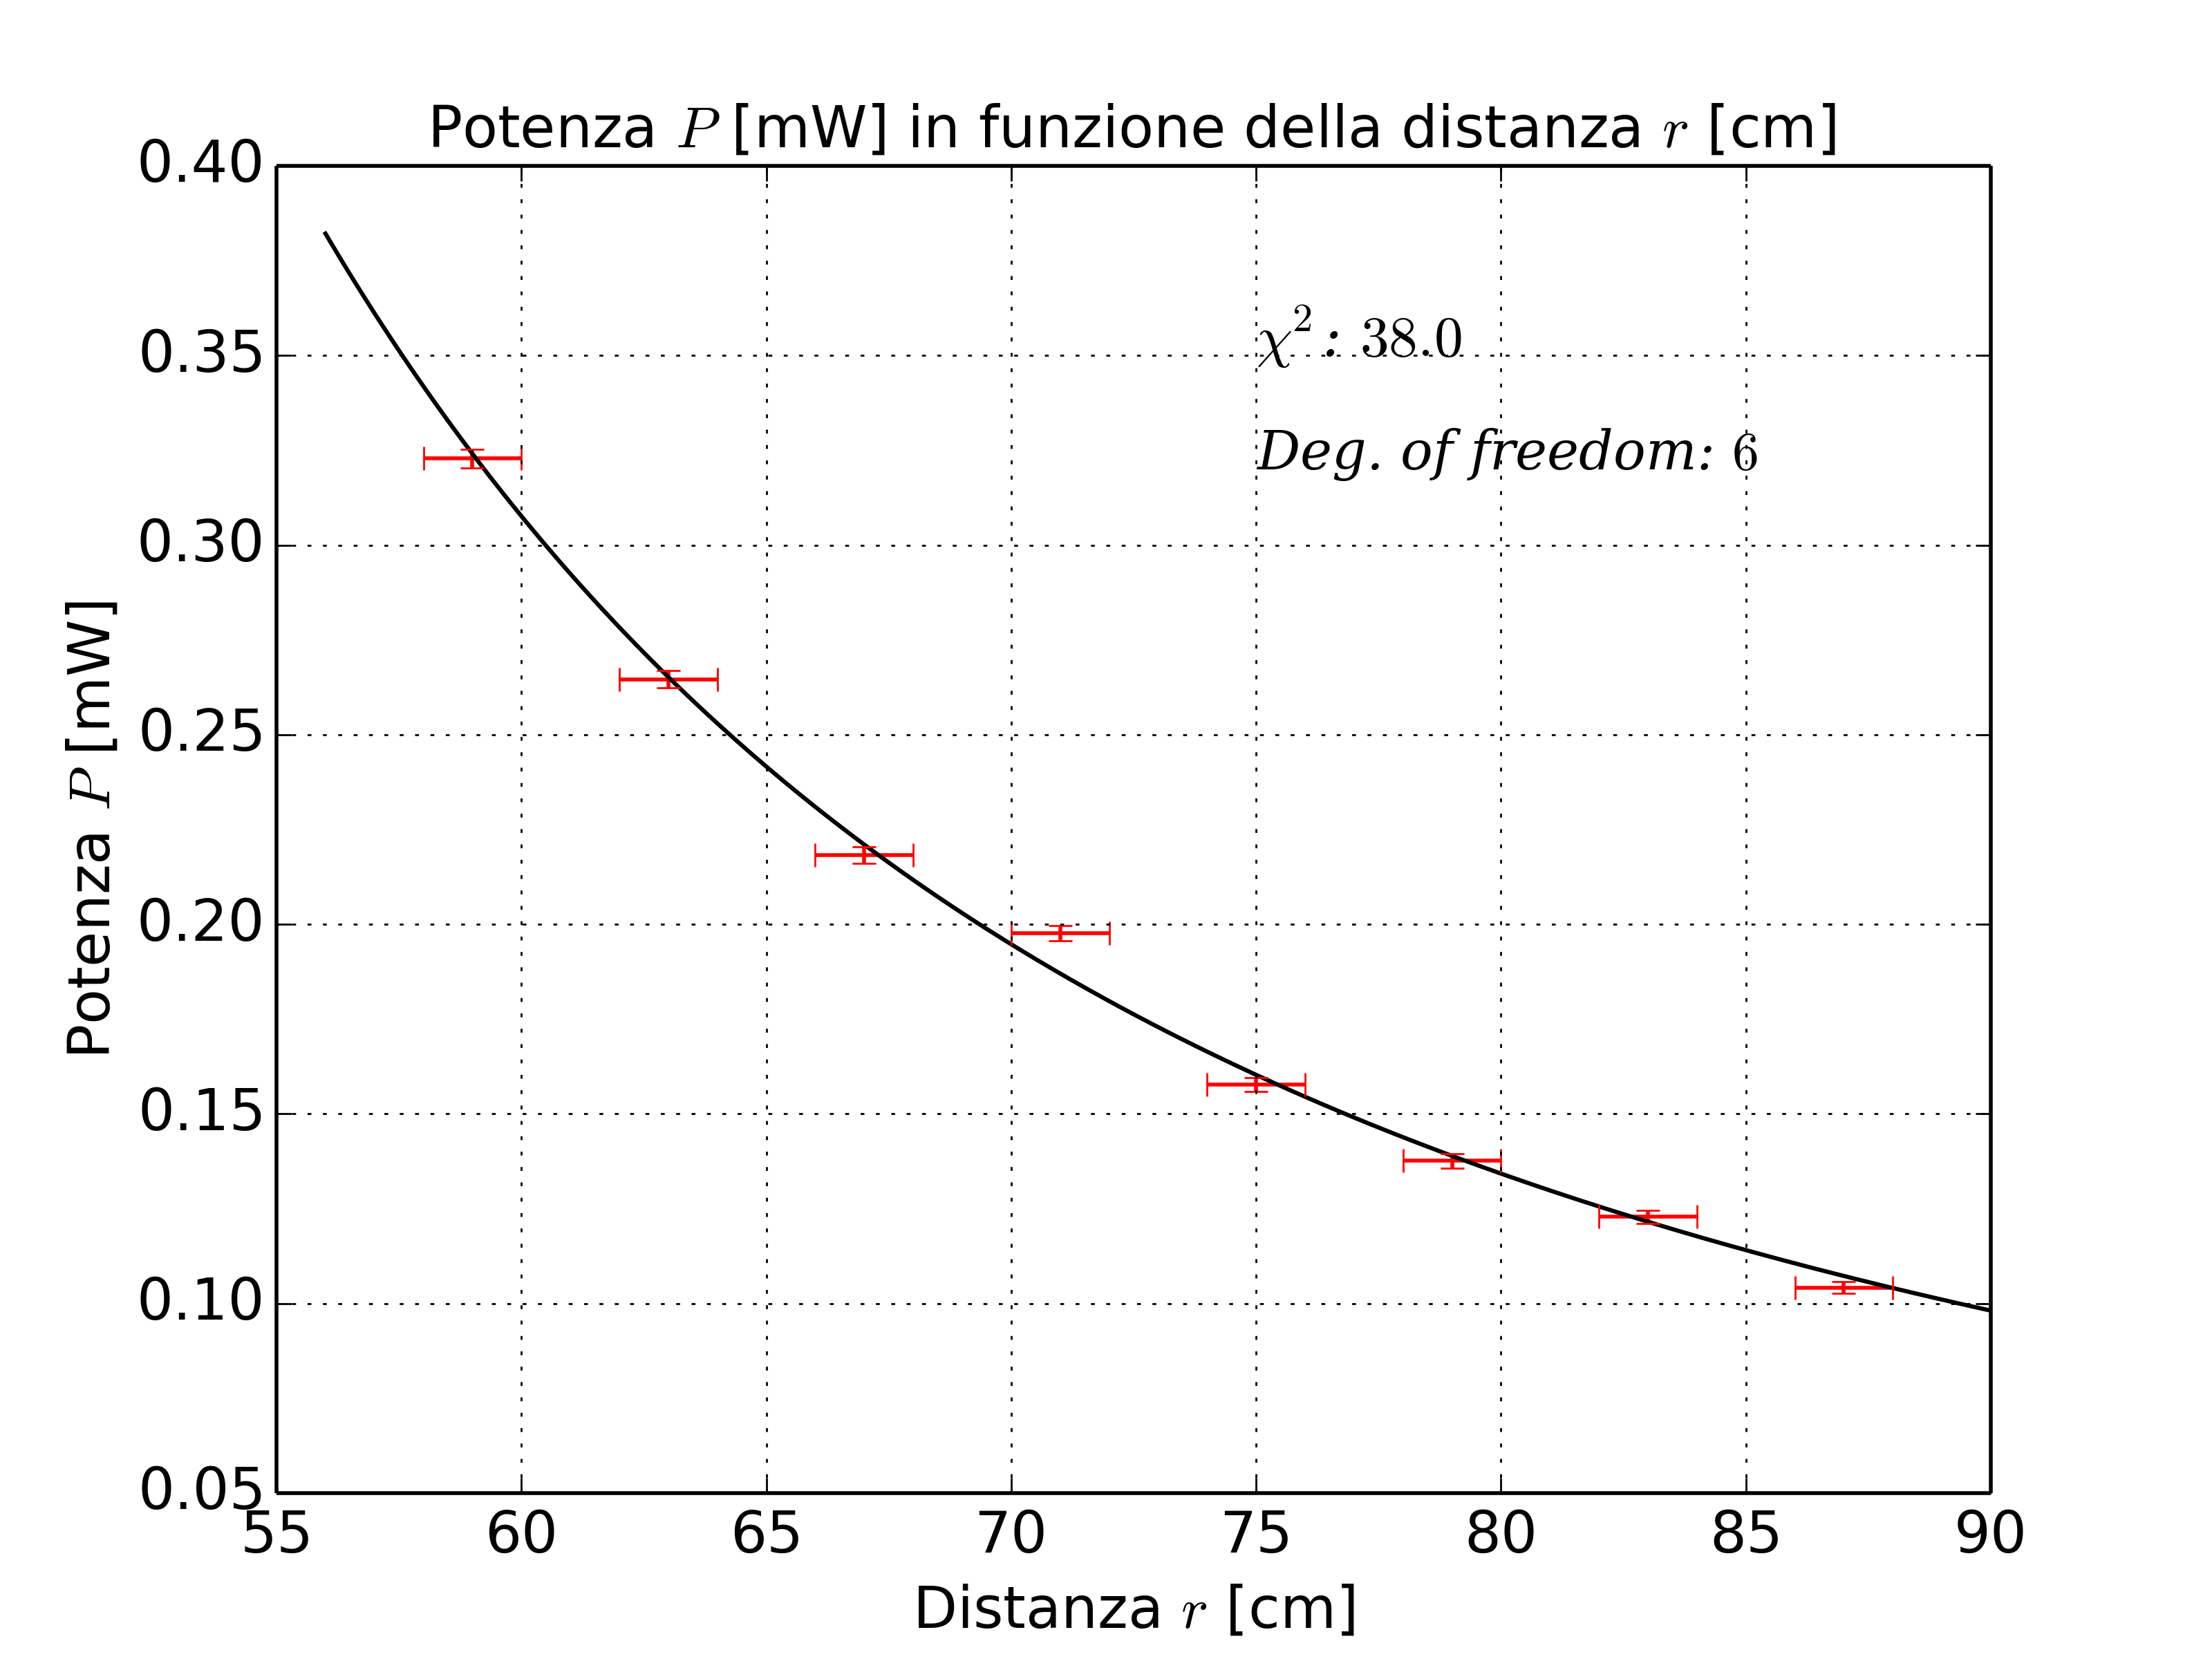
\includegraphics[width=0.8\linewidth]{./es7_fit_fissexp}
\caption{Best-fit della potenza in funzione della distanza, ad esponente fissato}
\label{fig:es7_fit_fissexp}
\end{figure}

\begin{figure}
\centering
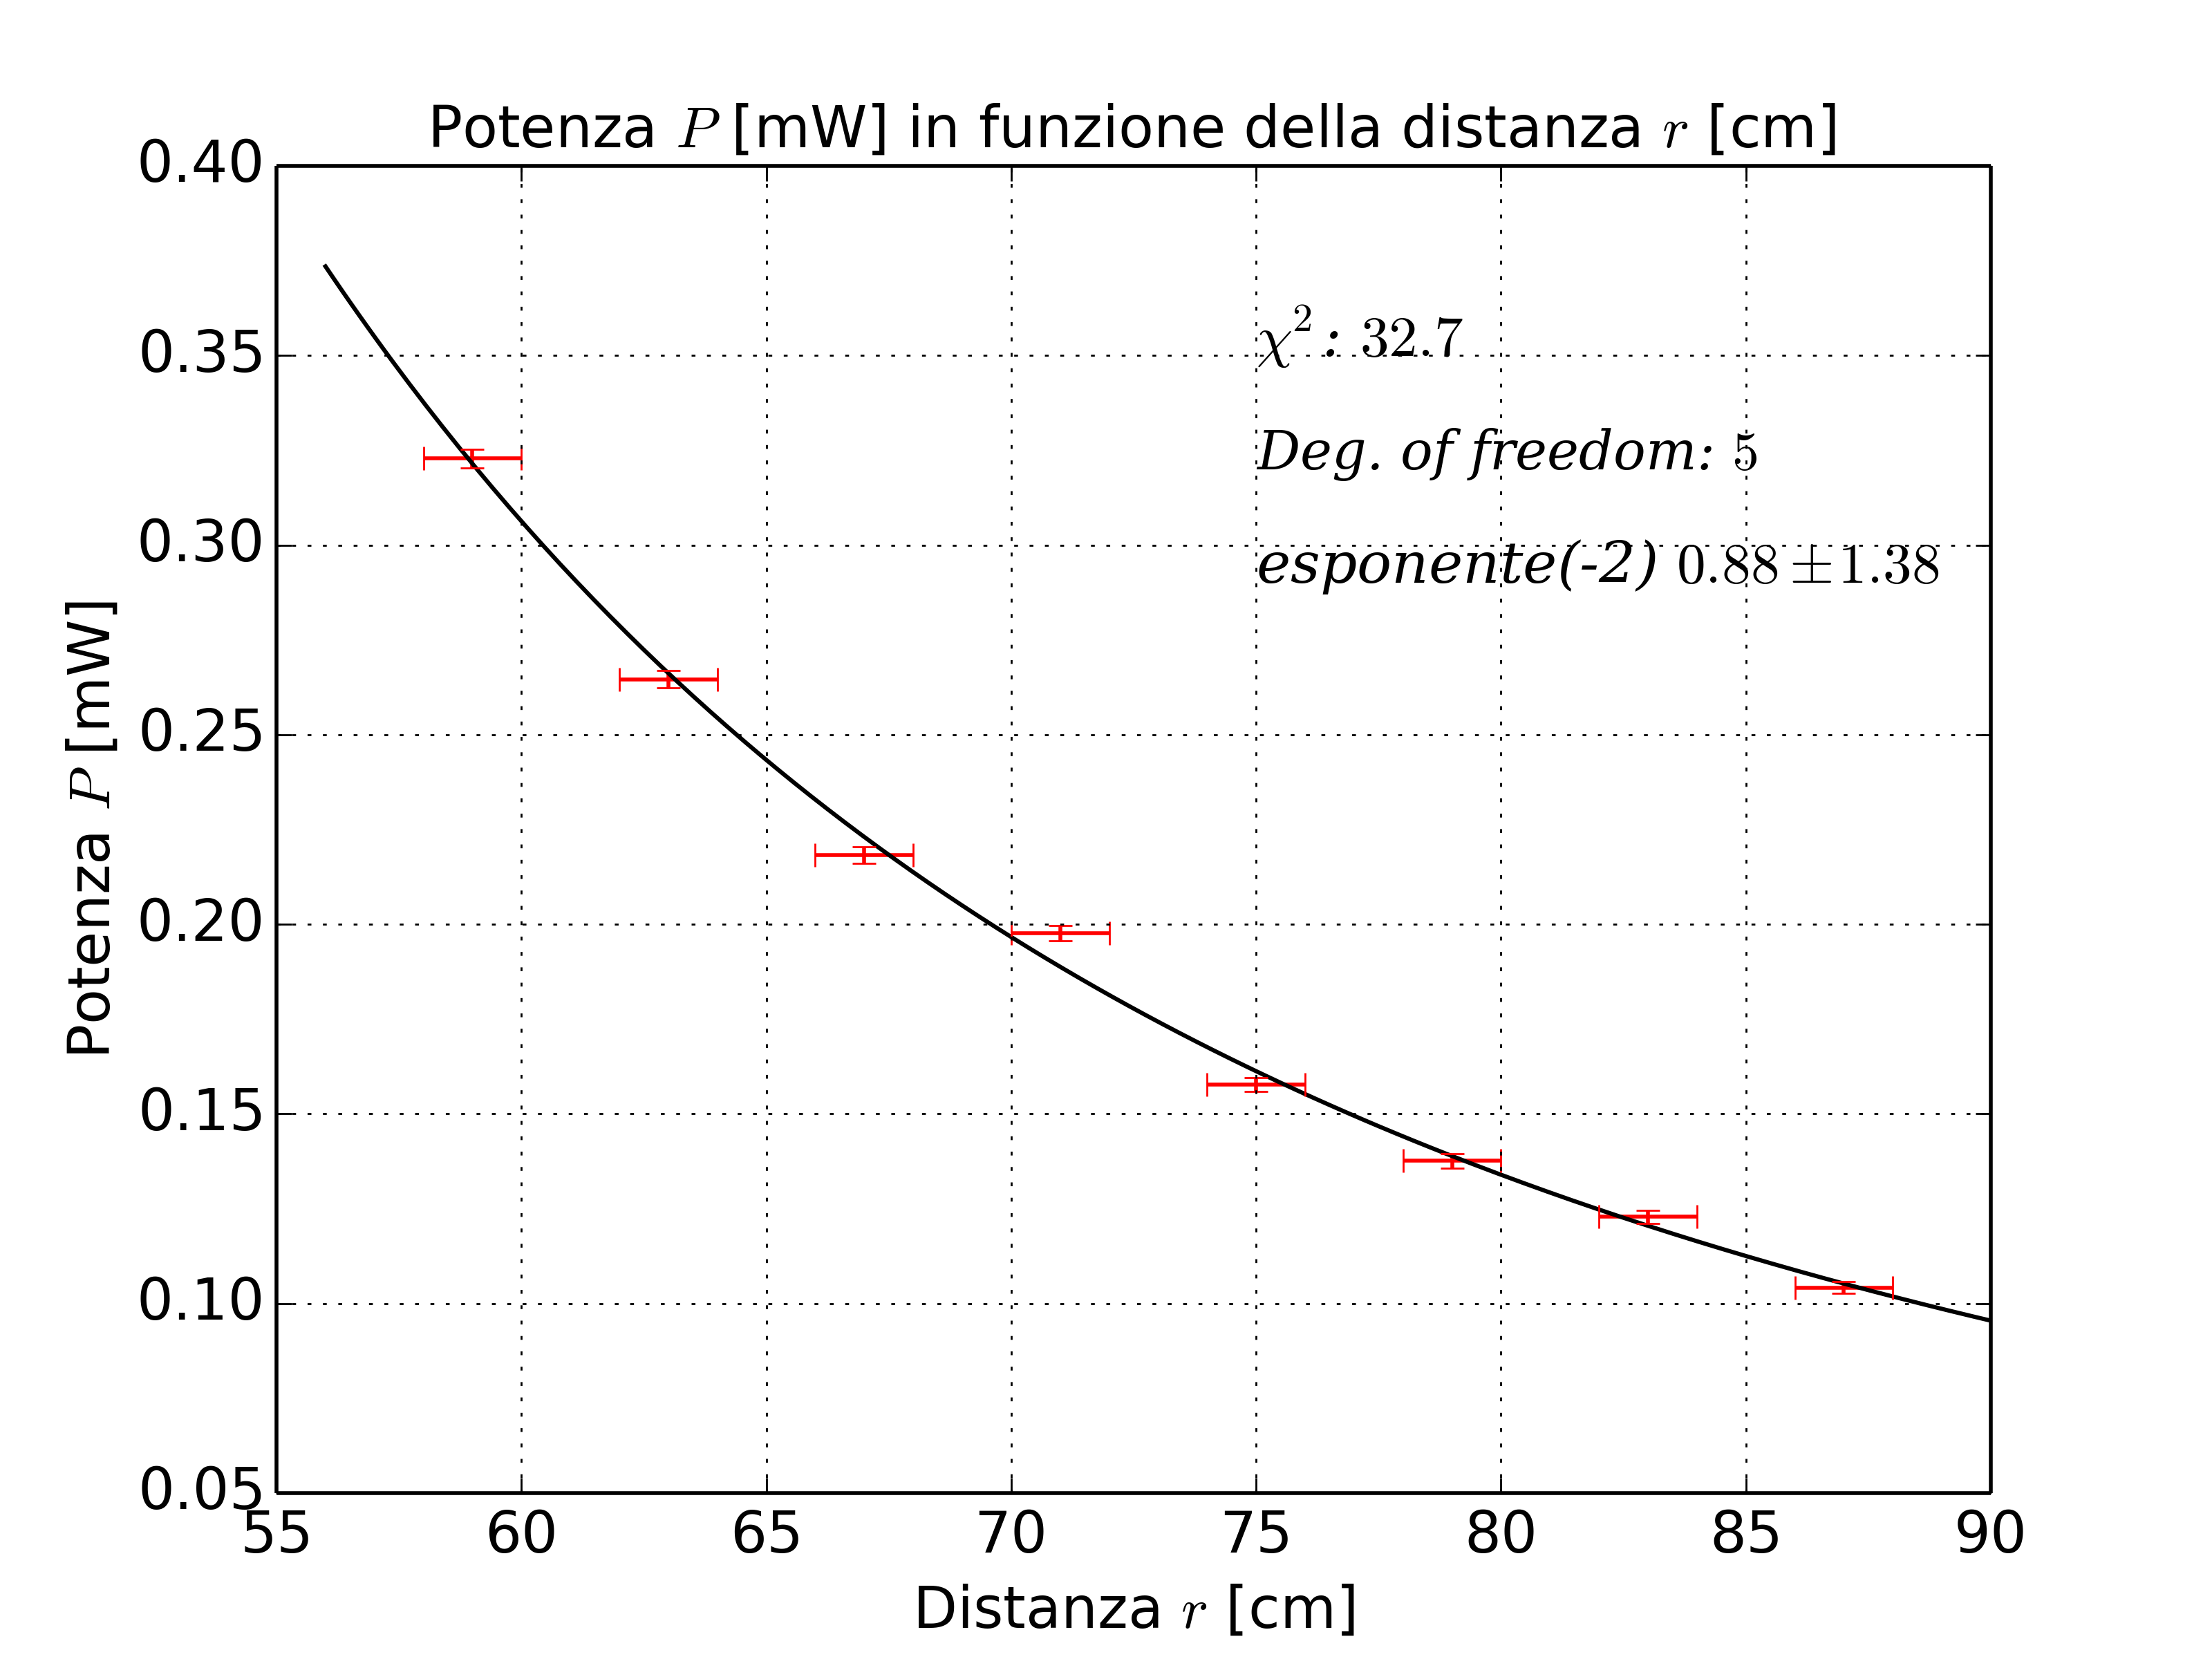
\includegraphics[width=0.8\linewidth]{./es7_fit_devexp}
\caption{Best-fit della potenza in funzione della distanza, ad esponente libero}
\label{fig:es7_fit_devexp}
\end{figure}


\section{Curva caratteristica - Filtri neutri}
Un'ulteriore prova può essere fatta interponendo dei filtri neutri fra la sorgente luminosa (in questo caso siamo ritornati alla torcia) e la cella fotovoltaica. A nostra disposizione ci sono 5 filtri \textit{Balzers} con attenuazione variabili comprese fra il 6.3 \% (frazione dell'intensità trasmessa) e il 97.4 \% (quindi molto poco attenuato). Le caratteristiche I-V sono riportate in Figura (\ref{fig:es_8_1}) con notazione analoga ai grafici precedenti.\\

\begin{figure}
\centering
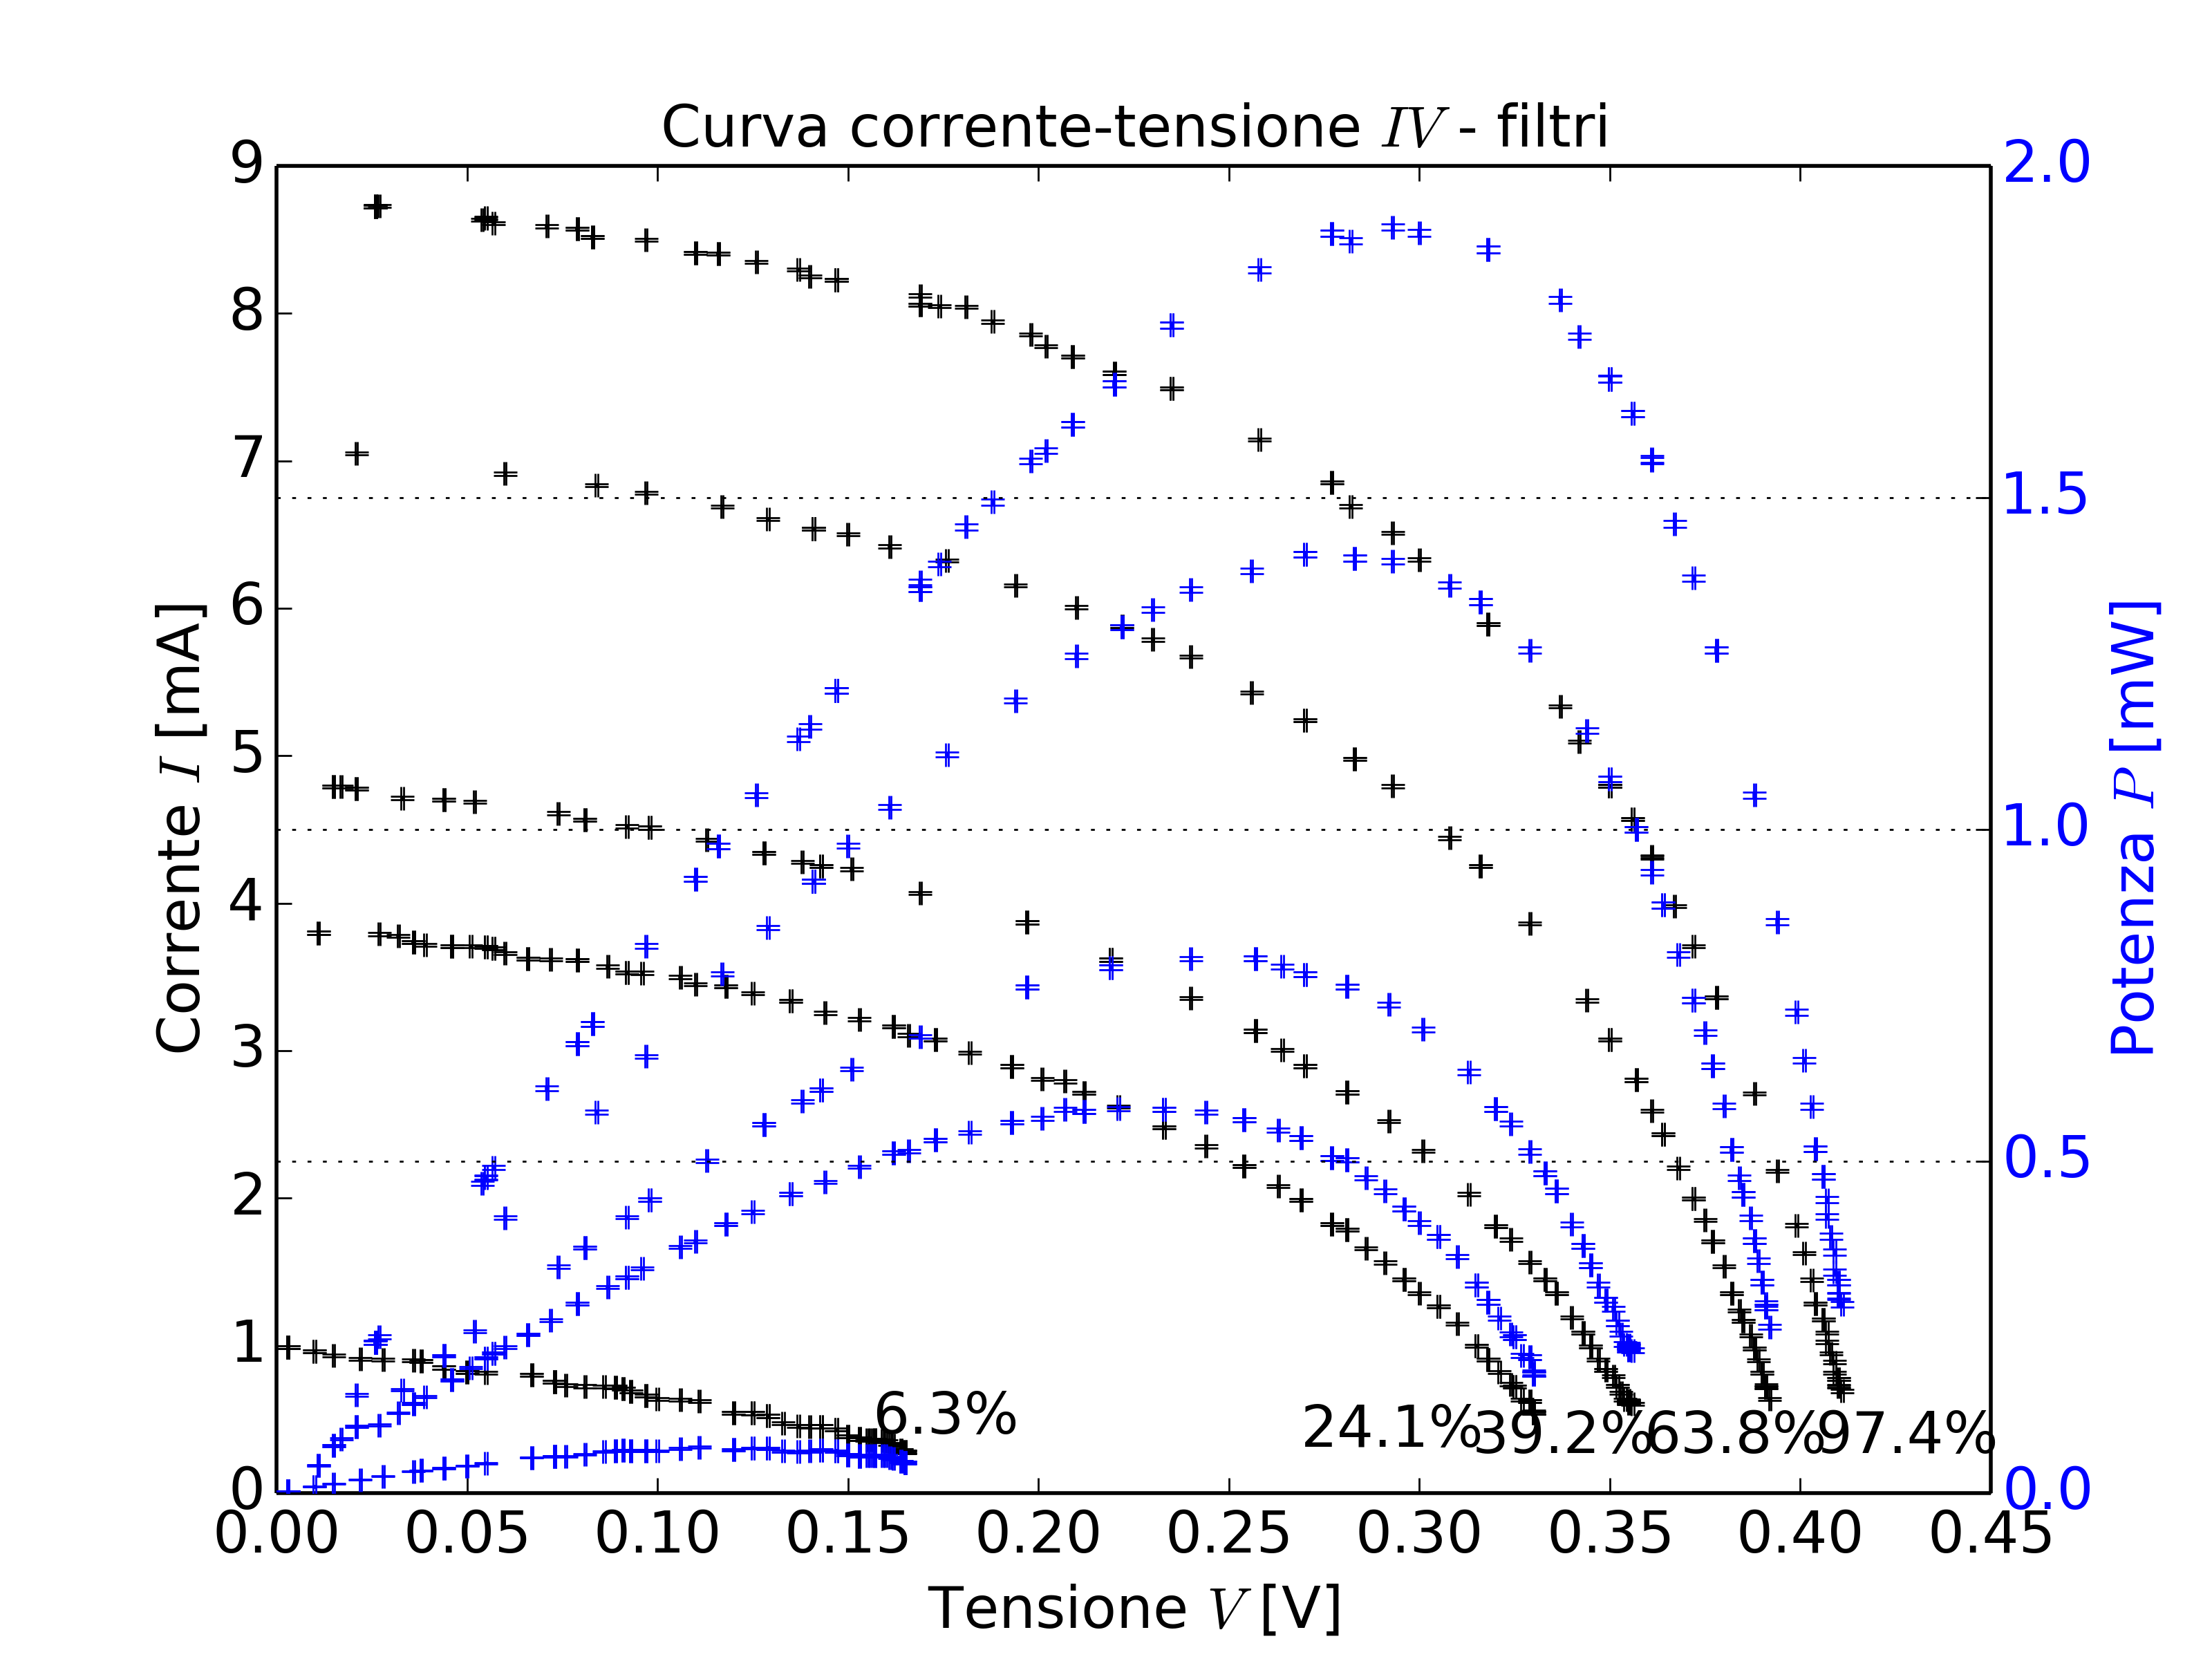
\includegraphics[width=0.9\linewidth]{./es_8_1}
\caption{Caratteristiche I-V per diversi filtri neutri.}
\label{fig:es_8_1}
\end{figure}

Si può osservare una (ovvia) diminuzione della potenza erogata tanto maggiore è l'attenuazione del filtro neutro. Può essere interessante riportare in una tabella i rapporti relativi fra le potenze massime e le attenuazioni dei filtri rispetto al filtro di attenuazione minima:\\

\begin{tabular}{|c|c|c|}
\hline \textbf{Filtro Balzers} & \textbf{Atten.} (norm.) & \textbf{Potenza max} (norm.) \\ 
\hline 97.4 \% & 1 & 1 \\ 
\hline 63.8\% & 0.66 & 0.74 \\ 
\hline 39.2\% & 0.40 & 0.42 \\ 
\hline 24.1\% & 0.25 & 0.30 \\ 
\hline 6.3\% & 0.06 & 0.04 \\ 
\hline 
\end{tabular} 

~\\
Notiamo una proporzionalità lineare (pur se non troppo precisa) fra l'attenuazione e la potenza massima erogata, come è lecito aspettarsi.\\
Infine, in Figura (\ref{fig:es_8_multi}) sono riportate le correnti massime e le tensioni massime, così come già definite, in funzione della potenza incidente. %Dal modello di Shockley si ricava facilmente una relazione 

\begin{figure}
\centering
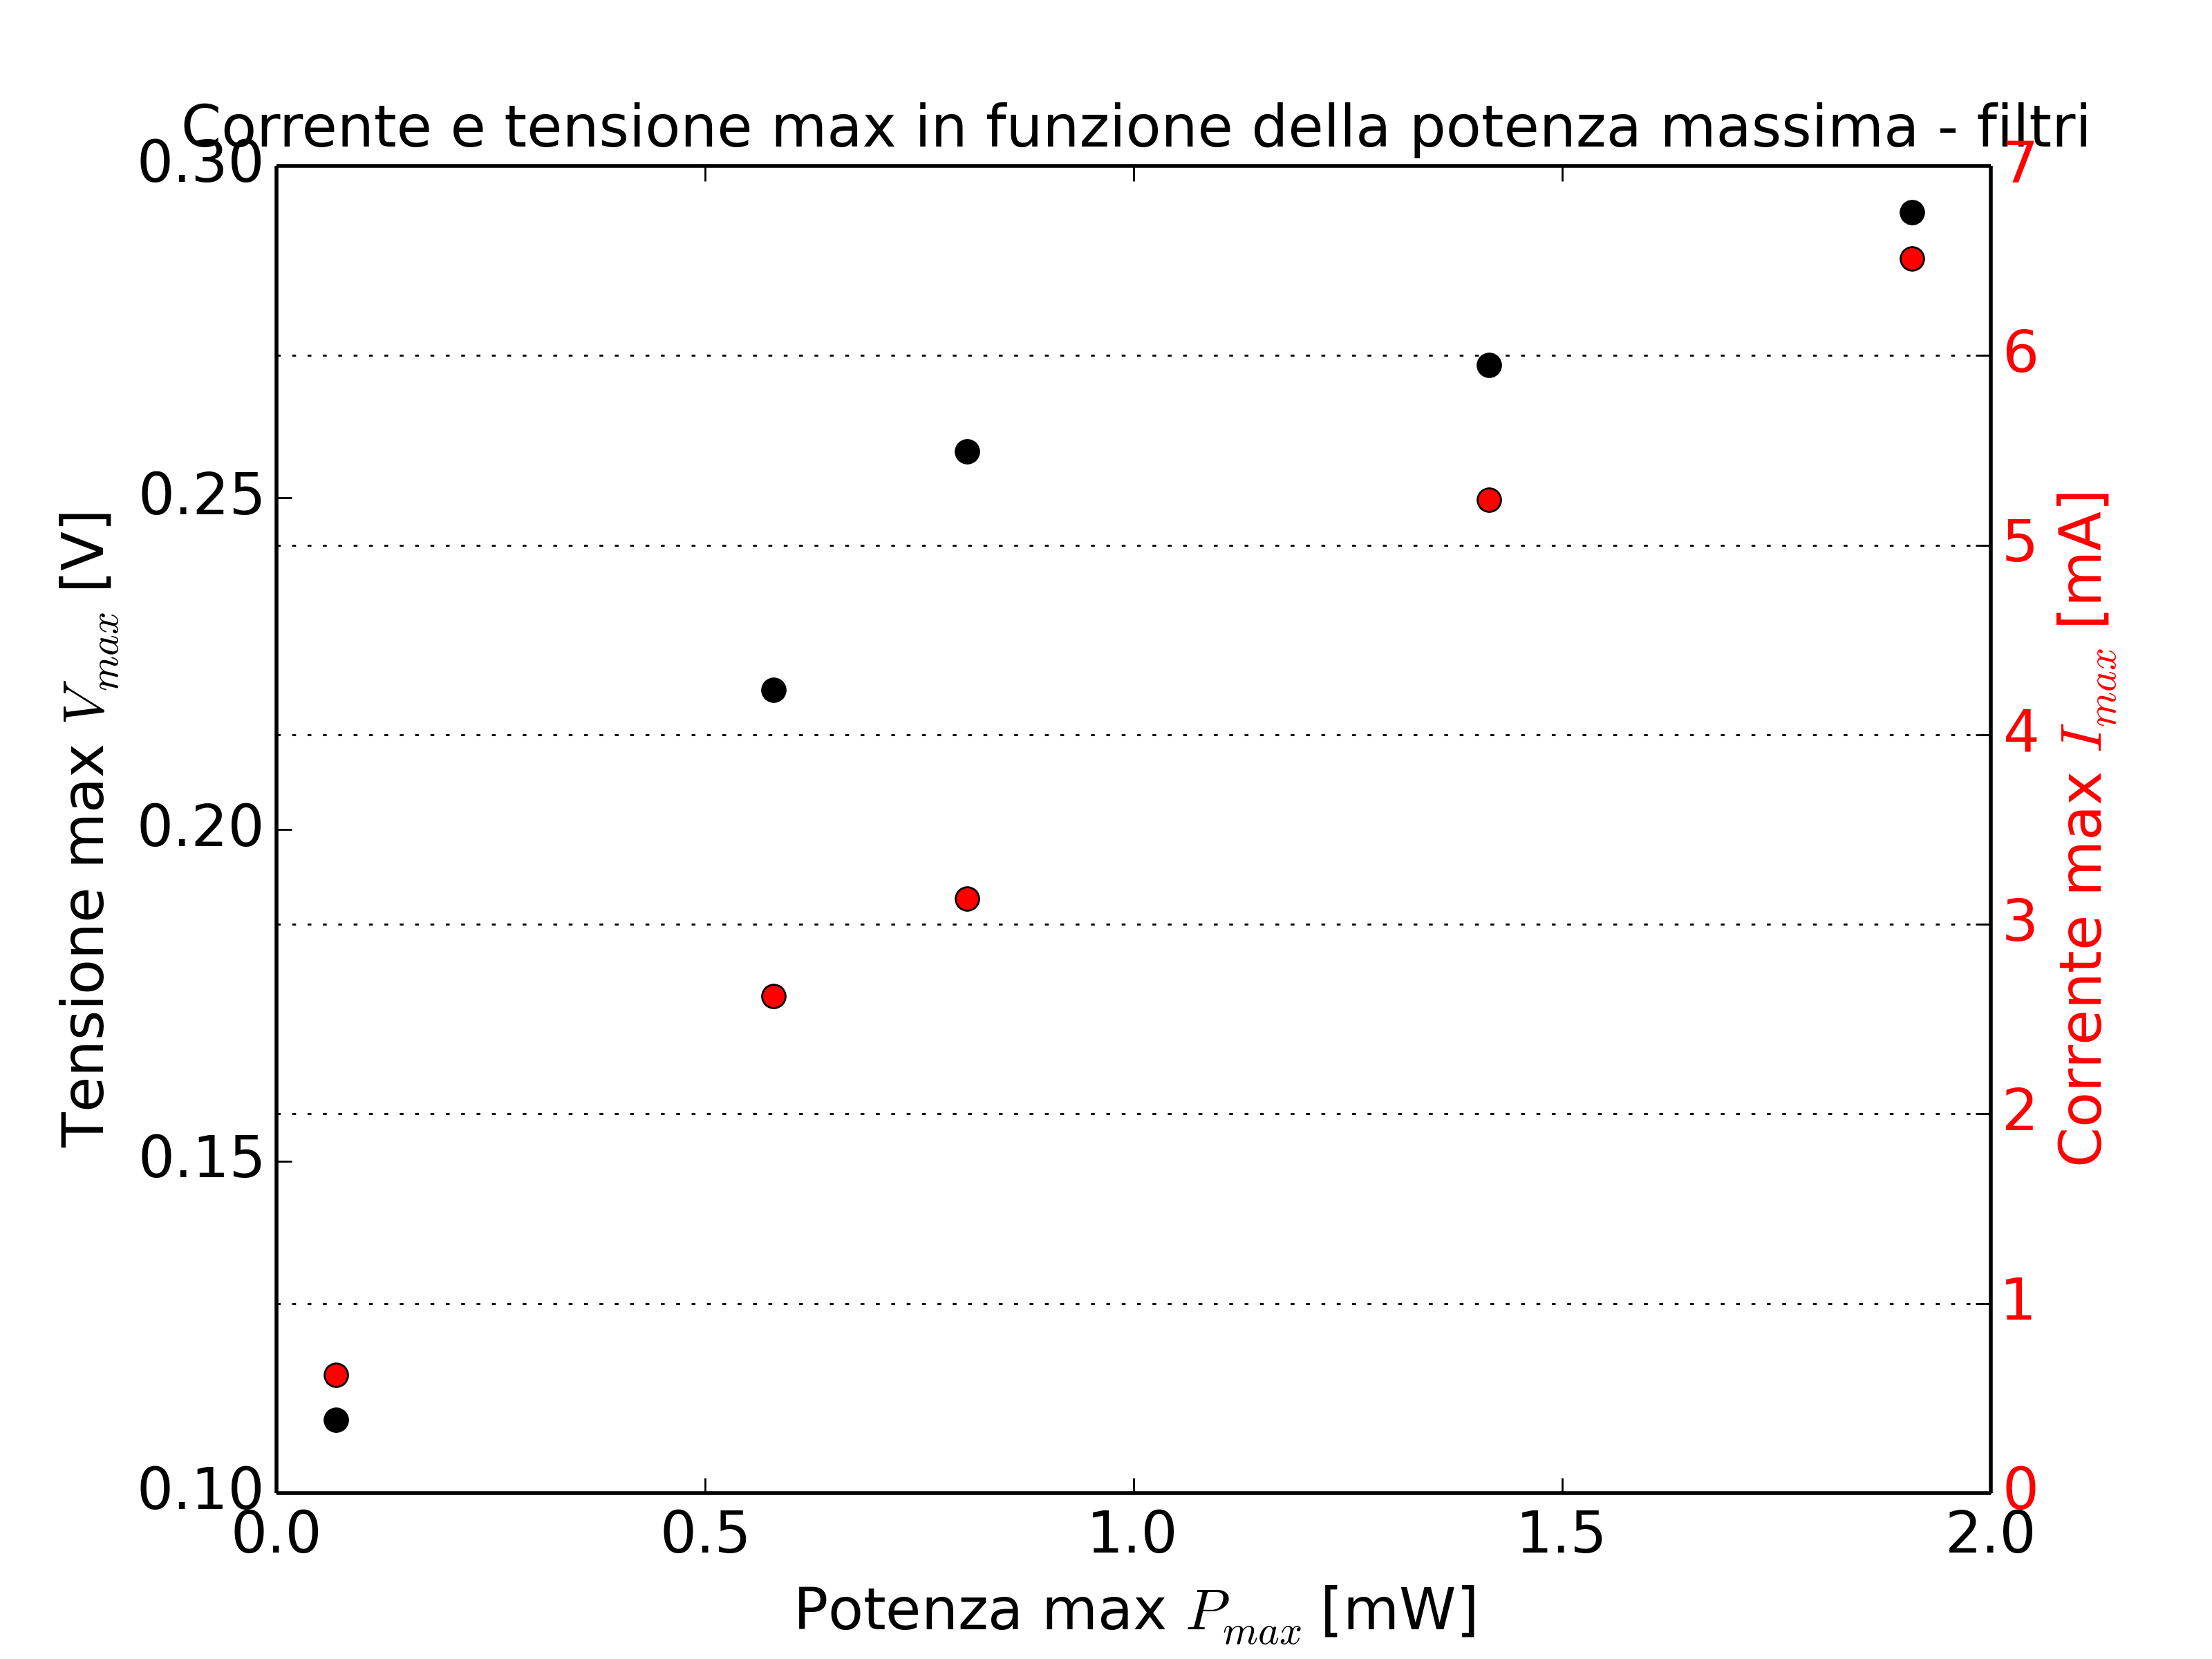
\includegraphics[width=0.9\linewidth]{./es_8_multi}
\caption{Corrente e Tensione massima in funzione della potenza max $P_{max}$.}
\label{fig:es_8_multi}
\end{figure}

Gli andamenti della corrente massima e della tensione massima rispetto alla $P_{max}$ sembrano essere, rispettivamente, lineare e logaritmico. Per verificarlo, si vedano in Figura (\ref{fig:es8_fit_corr},\ref{fig:es8_fit_tens}) i fit a due parametri liberi per entrambe le grandezze. Possiamo in qualche modo spiegarci questo andamento se facciamo riferimento al funzionamento di un fotodiodo (si veda la discussione nel logbook della week06) descritto dall'equazione:

\begin{equation}
I = I_s (\exp ^{\frac{V}{V_T}}-1)-I_{lux}
\end{equation}

dove $I_{lux}$ sta per la fotocorrente dovuta al'esposizione alla radiazione luminosa. Da questa è facile ricavare che in modalità fotovoltaica (I=0) la tensione $V$ va come il logaritmo della fotocorrente $V \propto ln(1+I_{lux}/I_s)$, che a sua volta è linearmente proporzionale all'illuminazione sul PD per il range di correnti da noi impiegato. In regime fotoconduttivo (V=0) la relazione fra $I$ e $Ill$ è invece lineare. Nei grafici riportati, questi comportamenti sono seguiti piuttosto bene dai dati sperimentali. 

\begin{figure}
\centering
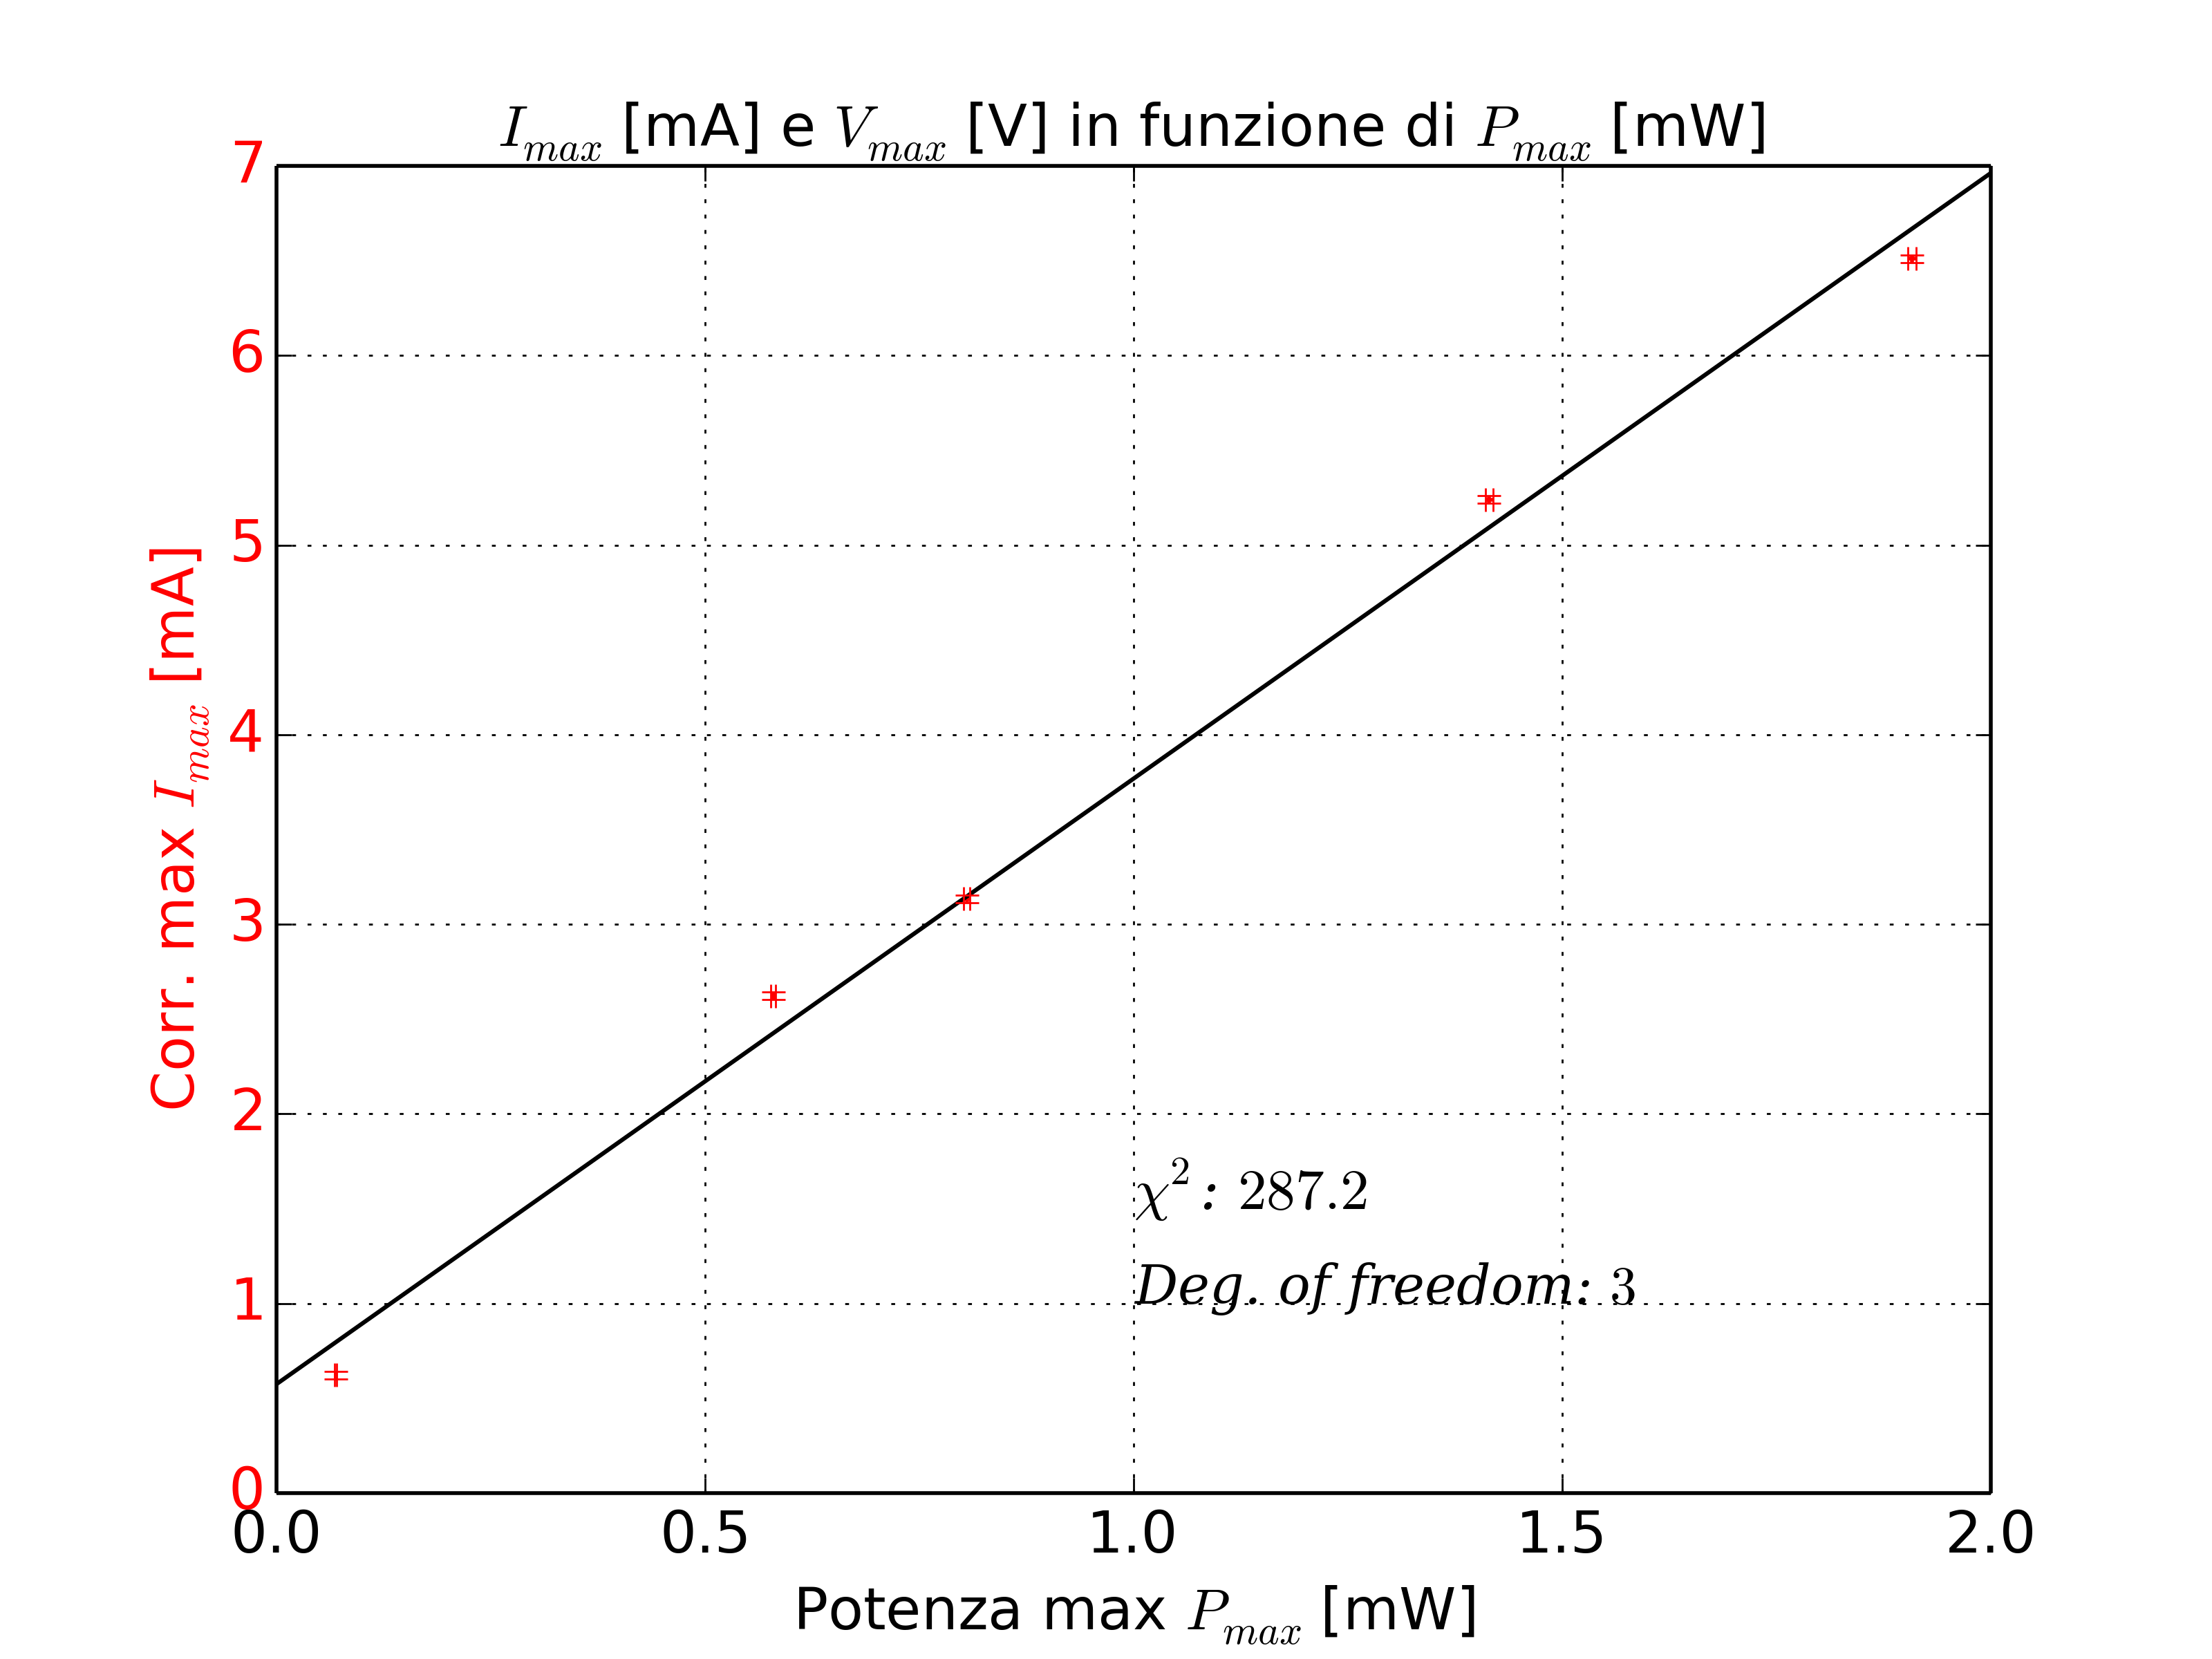
\includegraphics[width=0.8\linewidth]{./es8_fit_corr}
\caption{Fit lineare della corrente massima in funzione della potenza massima.}
\label{fig:es8_fit_corr}
\end{figure}

\begin{figure}
\centering
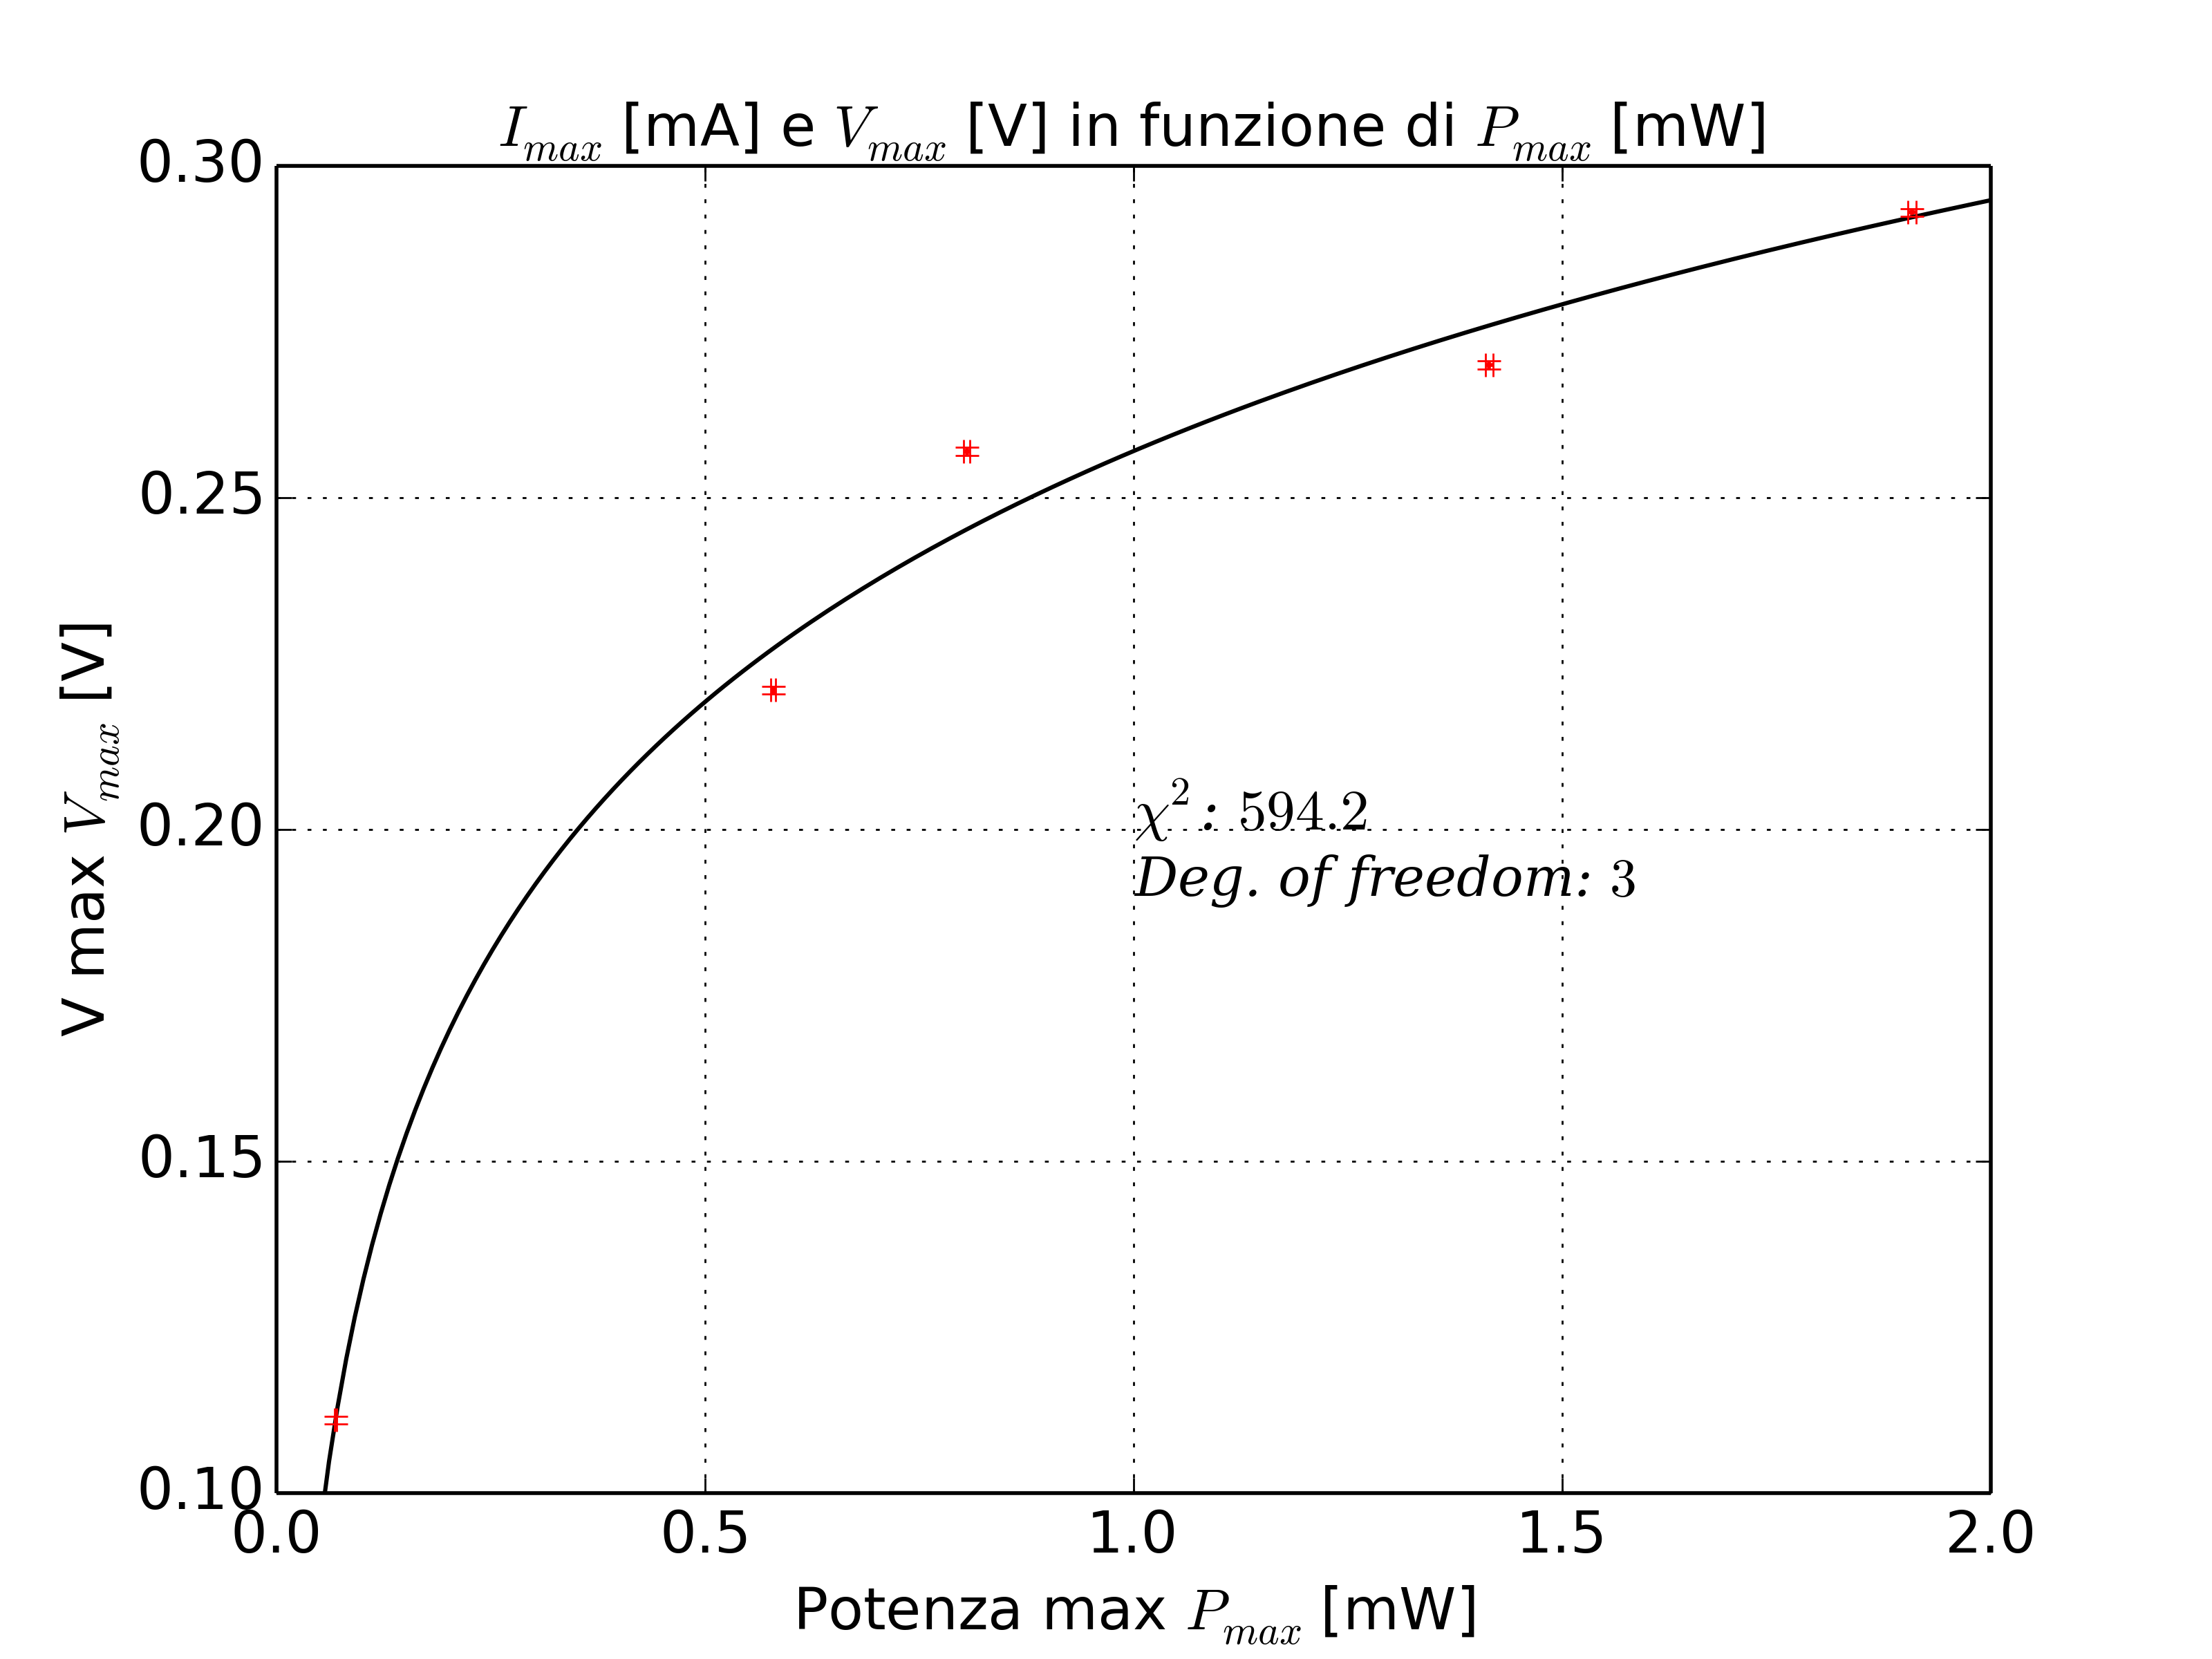
\includegraphics[width=0.8\linewidth]{./es8_fit_tens}
\caption{Fit logaritmico della tensione massima in funzione della potenza max.}
\label{fig:es8_fit_tens}
\end{figure}


\section{Curva caratteristica - superficie effettiva}
Per concludere, registriamo la curva I-V al variare della porzione illuminata della cella, coprendo la superficie con un cartone rigido. Per ragioni di tempo, sono state effettuate solo tre misure: una di riferimento con superficie comletamente esposta, l'altra con metà superficie esposta e l'ultima con un quarto.\\

Si riportano in Figura (\ref{fig:es_9corr_v}) i valori di corrente massima e di tensione massima in funzione della superficie (normalizzata a 1): si nota un andamento circa lineare. Questo potrebbe essere confermato dal grafico in Figura (\ref{fig:es_9pot_sup}) dove invece è riportata la potenza massima in funzione della superficie esposta. In questo caso l'andamento sembra più di tipo quadratico, anche se, ovviamente, tre punti sperimentali sono del tutto insufficienti per trarre delle conclusioni rigorose. 

\begin{figure}
\centering
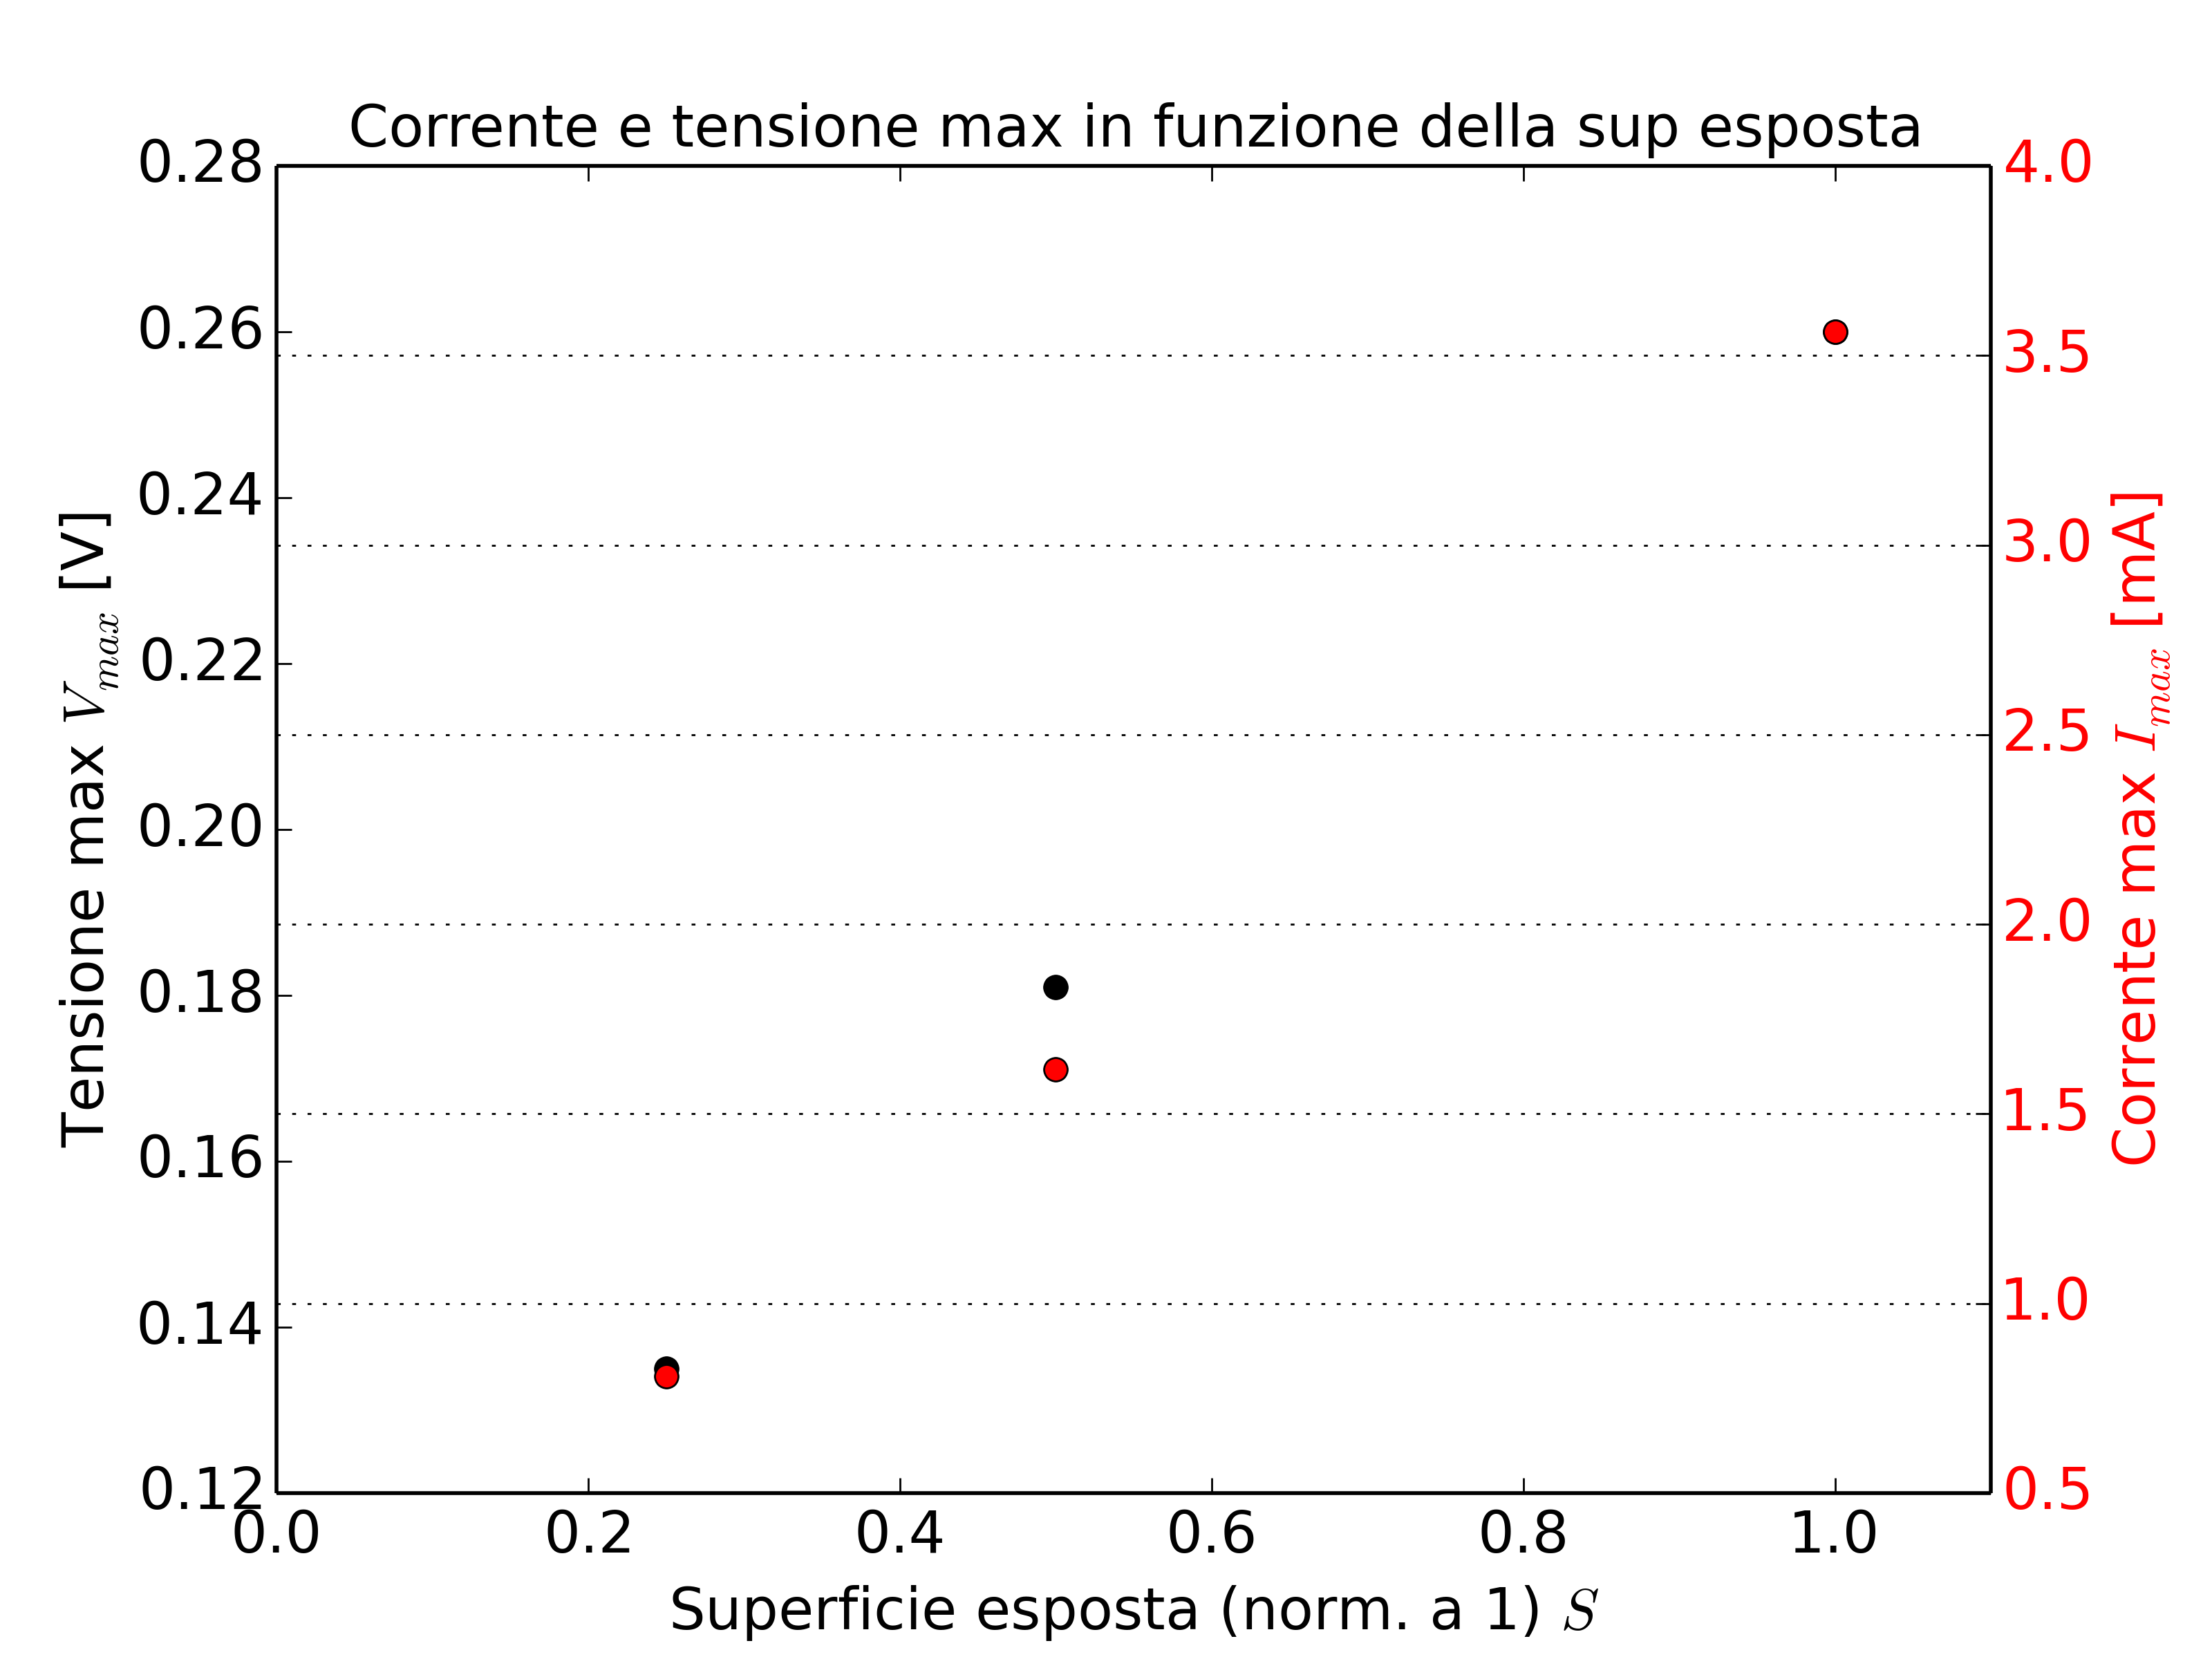
\includegraphics[width=0.9\linewidth]{./es_9corr_v}
\caption{Andamento della tensione massima e della corrente massima in funzione della superficie esposta.}
\label{fig:es_9corr_v}
\end{figure}

\begin{figure}
\centering
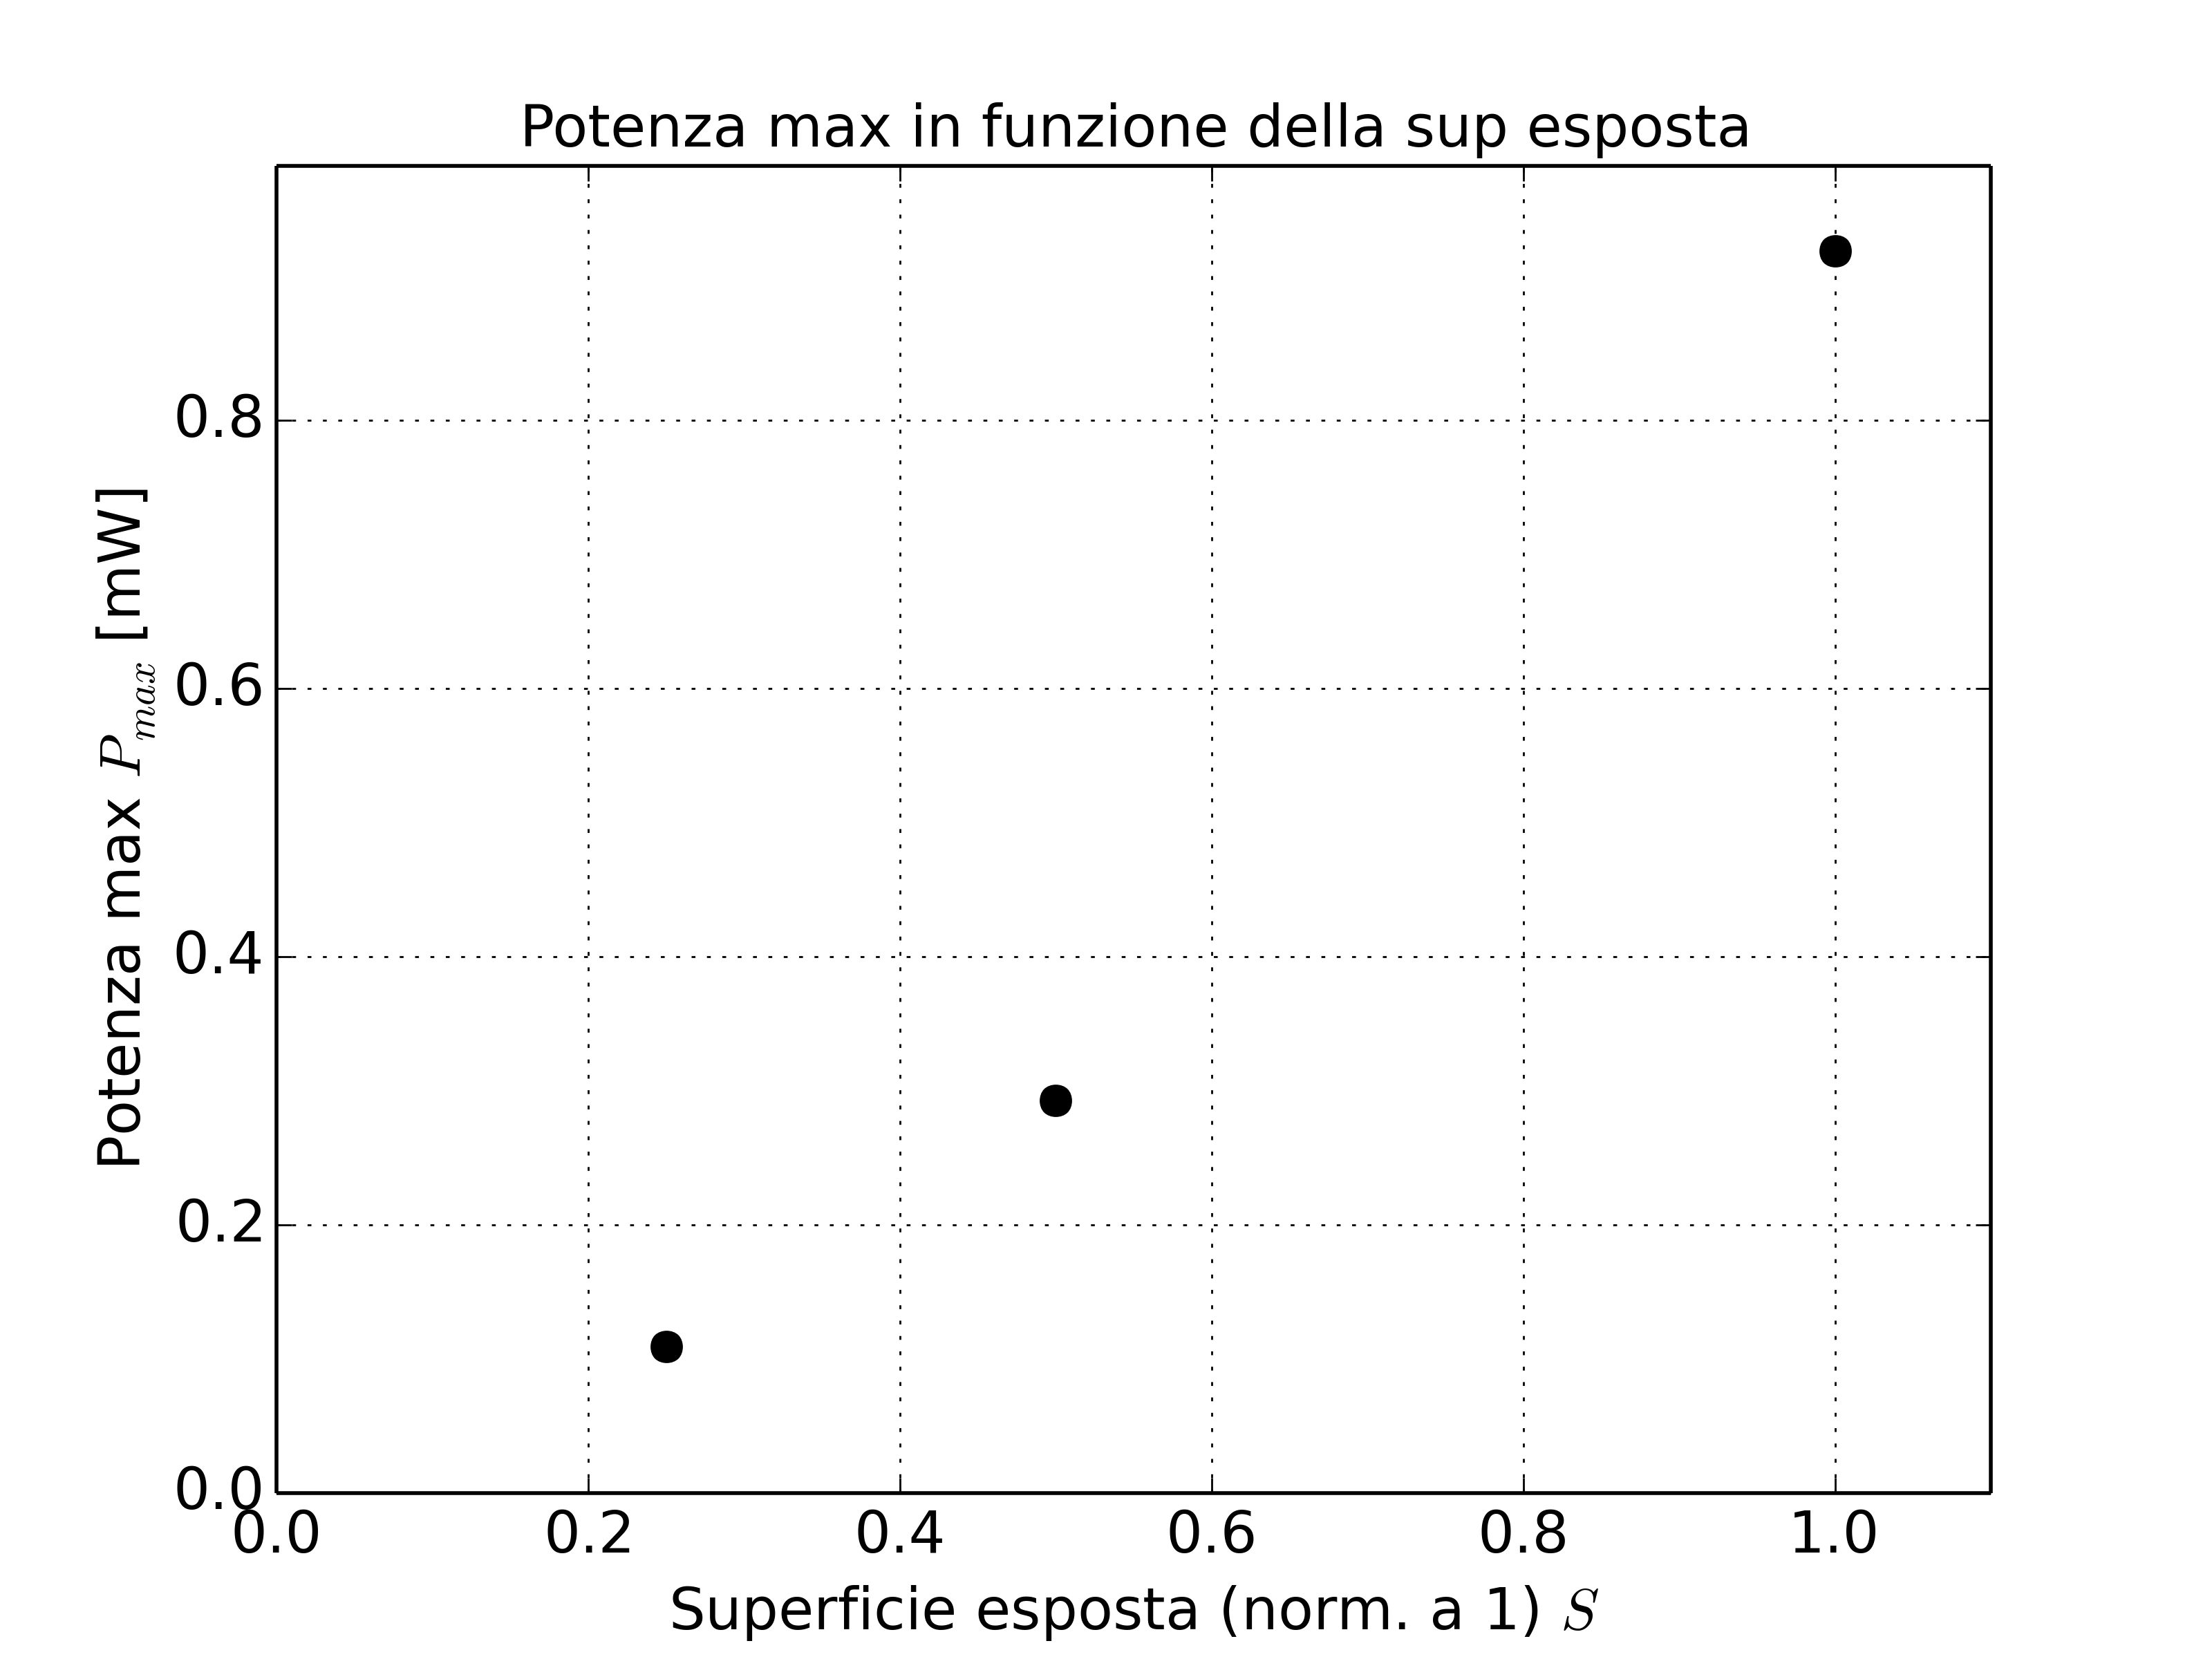
\includegraphics[width=0.9\linewidth]{./es_9pot_sup}
\caption{Andamento della potenza massima in funzione della superficie esposta}
\label{fig:es_9pot_sup}
\end{figure}

\section{BONUS - Risposta della cella ad una sorgente luminosa colorata}
Prima di iniziare l'esperienza, avevamo già verificato la diversa differenza di potenziale ai capi della cella indotta da immagini monocromatiche di vario colore proiettate sullo schermo del monitor. Sappiamo, inoltre, che le celle solari basate su giunzione a silicio possiedono una curva di responsività in funzione della lunghezza d'onda della radiazione incidente: in particolare la curva è calibrata sullo spettro visibile della radiazione del sole, con un picco sul giallo-verde.\\
In questa sezione tale fenomeno verrà esaminato approfonditamente e in maniera rigorosa.\\

E' stato preparato uno script per Matlab/Octave che mostrasse in sequenza sullo schermo i colori corrispondenti alle possibili combinazioni RGB (red-green-blue), vale a dire i colori che è possibile visualizzare sui dispositivi digitali, preceduti e seguiti dal colore nero, come riferimento per la cella. La sequenza di colori dura 3s, ogni colore intervallato dall'altro per un centesimo di secondo. La sequenza è come segue:\\

\begin{table}
\centering
\begin{tabular}{|c|c|c|}
\hline \textbf{R} &\textbf{ G} & \textbf{B} \\ 
\hline 1 & 0 & 0 \\ 
\hline 1 & 0.1 & 0 \\ 
\hline 1 & 0.2 & 0 \\ 
\hline . & . & . \\ 
\hline . & . & . \\ 
\hline 1 & 1 & 0 \\ 
\hline 0.9 & 1 & 0 \\ 
\hline 0.8 & 1 & 0 \\ 
\hline . & . & . \\ 
\hline . &.  & . \\ 
\hline 0 & 1 & 0 \\ 
\hline 0 & 1 & 0.1 \\ 
\hline 0 & 1 & 0.2 \\ 
\hline . & . & . \\ 
\hline . & . & . \\ 
\hline 0 & 1 & 1 \\ 
\hline 0 & 0.9 & 1 \\ 
\hline . & . & . \\ 
\hline 0 & 0 & 1 \\ 
\hline 0.1 & 0 & 1 \\ 
\hline . & . & . \\ 
\hline 1 & 0 & 1 \\ 
\hline . & . & . \\ 
\hline 
\end{tabular} 
\end{table}
~\\

Abbiamo quindi appoggiato la cella sul monitor, avviato lo script e acquisito la tensione con il VI \textit{TracciaVinVout2}, ponendo come resistenza di carico al posto del potenziometro (oltre quella di campionamento) $R = 50 \Omega$, in modo da trovarci come punto di lavoro il più vicino possibile alle condizioni di potenza erogata massima. La frequenza di campionamento è stata posta pari a 2000Sample/s. Di seguito è riportato il grafico con l'acquisizione delle tensioni in funzione del tempo (Figura (\ref{fig:1_dati_sperimentali})).\\

\begin{figure}
\centering
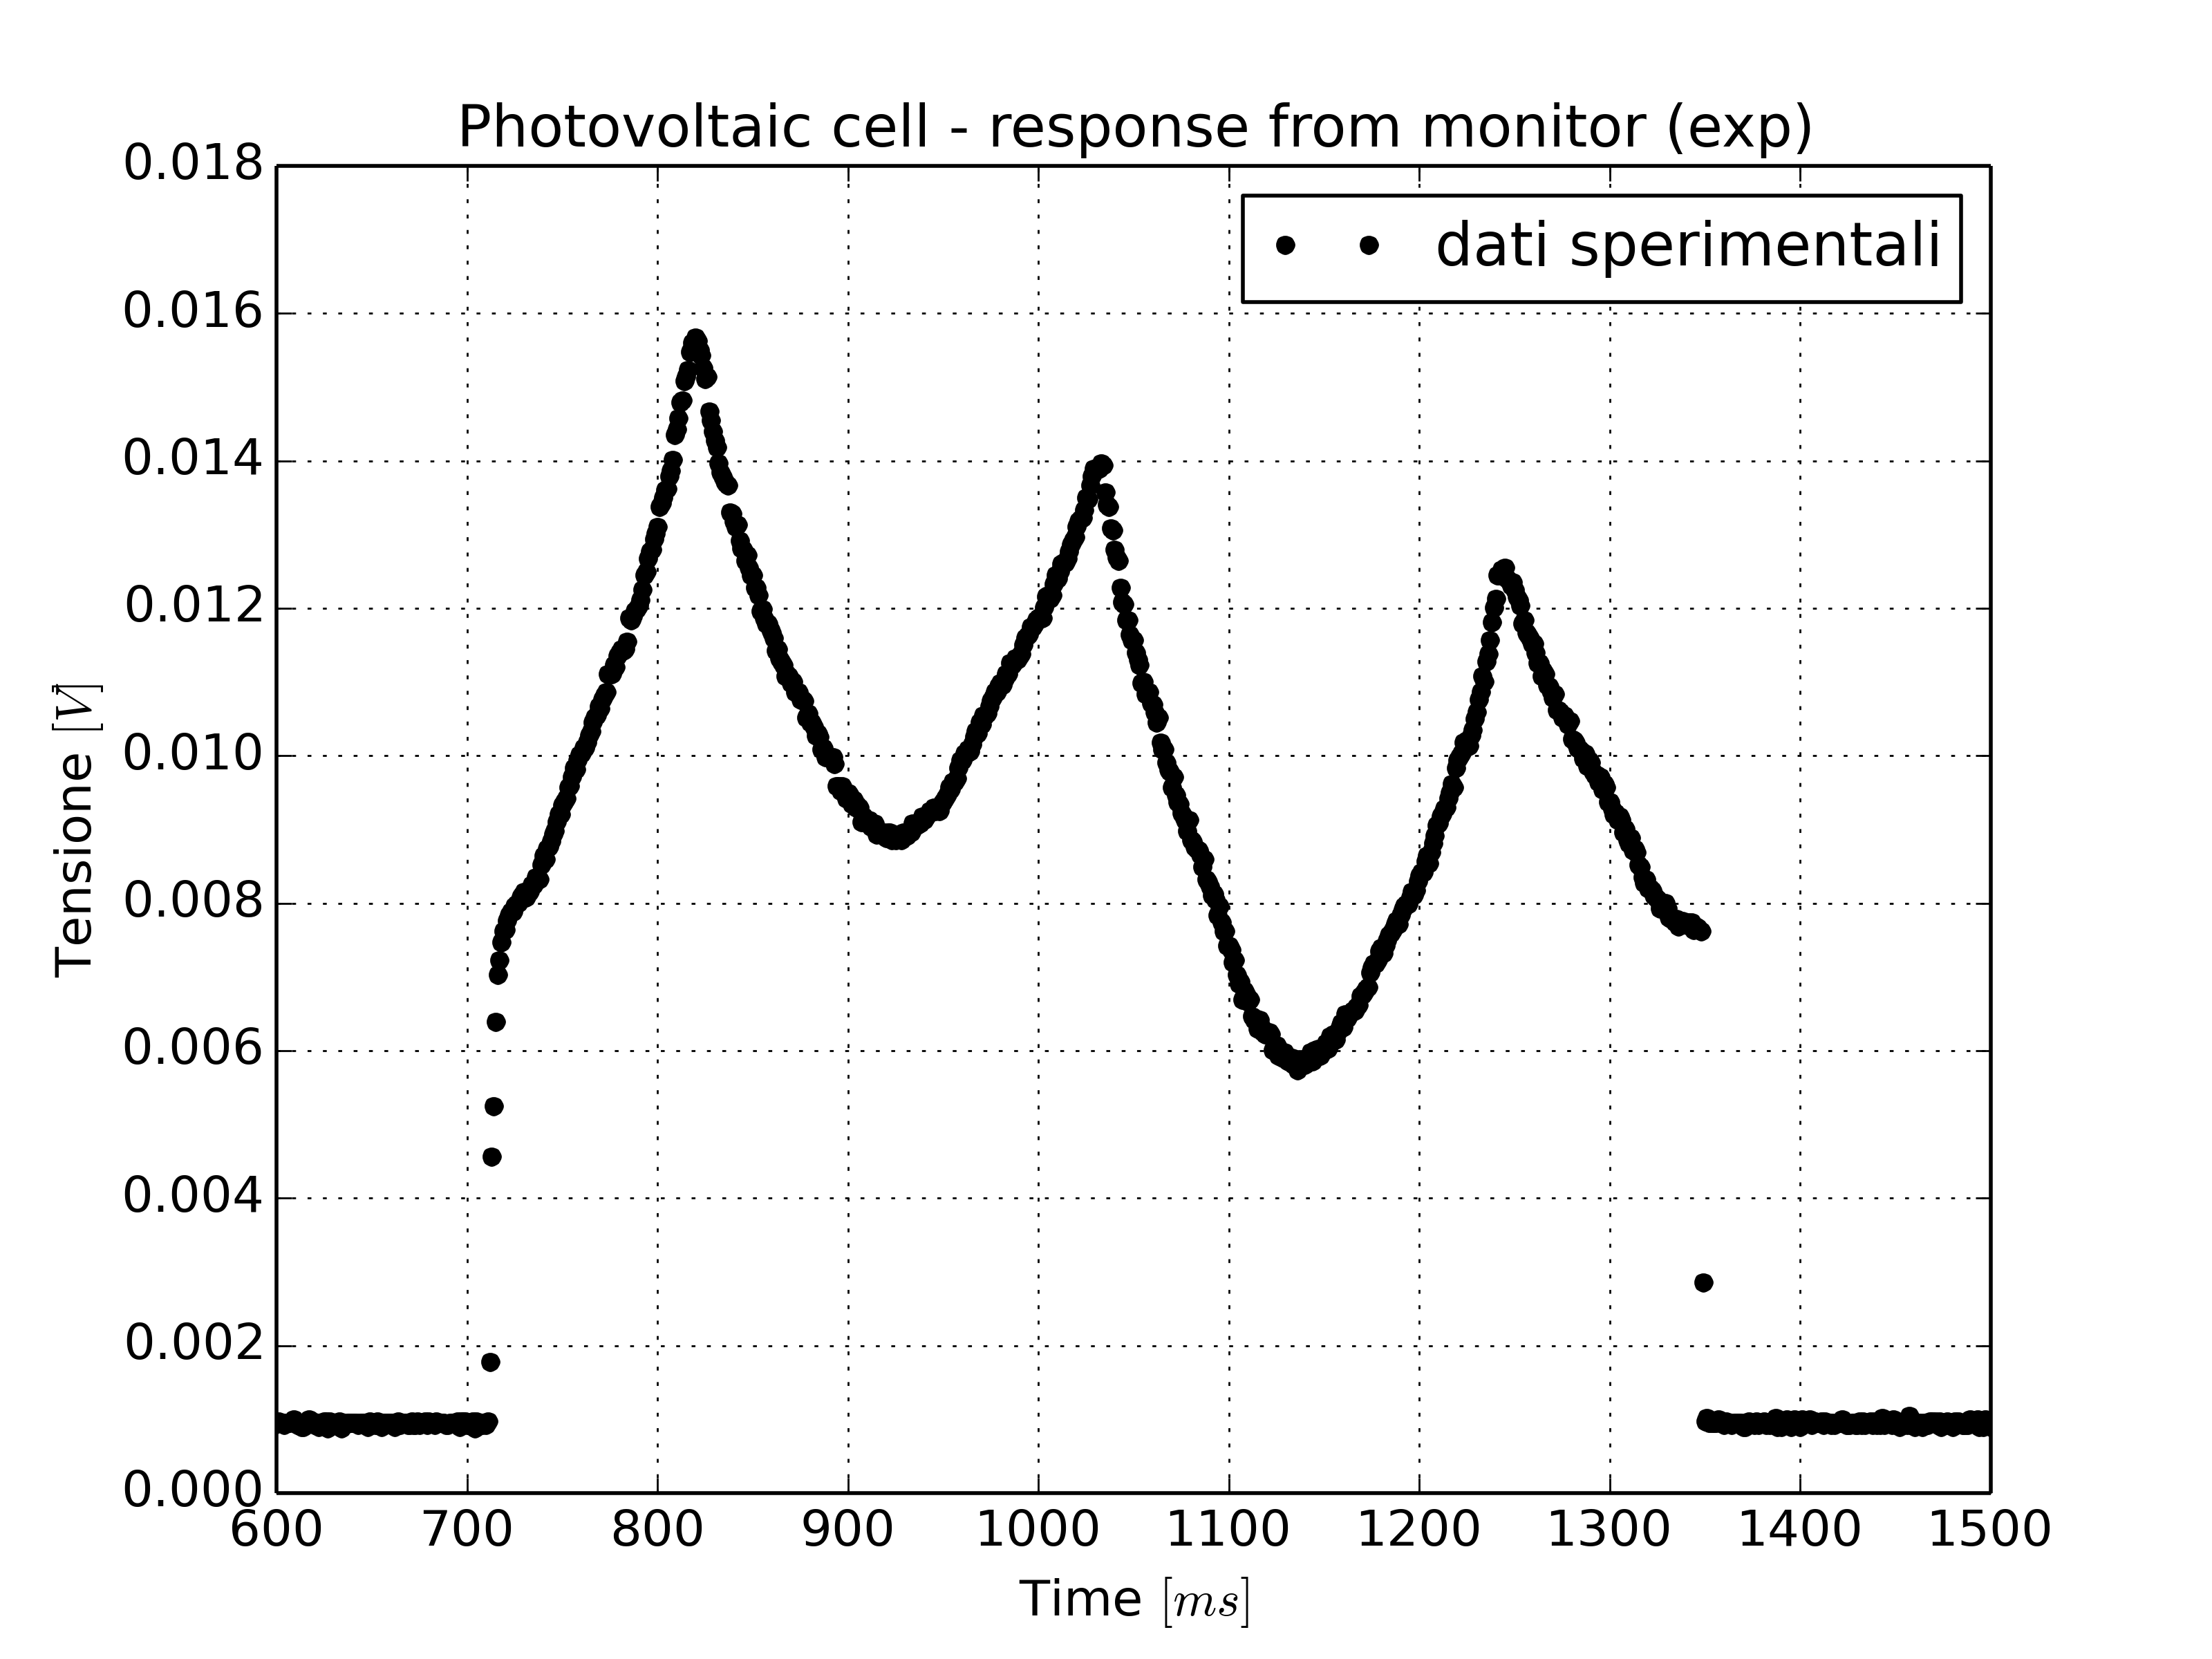
\includegraphics[width=0.8\linewidth]{./relaz_colori/1_dati_sperimentali}
\caption{Tensione ai capi della cella in funzione del tempo}
\label{fig:1_dati_sperimentali}
\end{figure}


Il grafico presenta tre picchi molto evidenti, intervallati da delle concavità accentuate: la figura è chiaramente diversa dalla risposta spettrale di una cella fotovoltaica. La prima ipotesi per spiegarci i picchi è stata quella di attribuirli alle combinazioni RGB di colore rosso, verde e blu, rispettivamente. Questo perchè, si è pensato, queste sono le triplette in cui tutti i pixel sono accesi dello stesso colore. Le concavità, invece, sarebbero potute essere dovute al fatto che quando i pixel sono accesi di più colori (una combinazione RGB) le luminosità di ciascuno potrebbero essere ridotte per ottenere una resa visiva ottimale.\\
Tuttavia, una successiva valutazione della struttura del pixel e del suo funzionamento ci ha portati a cambiare idea. Infatti, ogni pixel è costituito da tre diverse sub-unità, approssimabili a tre LED, di cui ognuno di questi può accendersi di un solo colore, appunto rosso, verde e blu. In particolare, quando si deve produrre il colore rosso, solo il LED corrispondente verrà acceso, al massimo della sua intensità, mentre gli altri due rimangono spenti. Ciò è visibile in Figura (\ref{fig:pixelRED}).

\begin{figure}
\centering
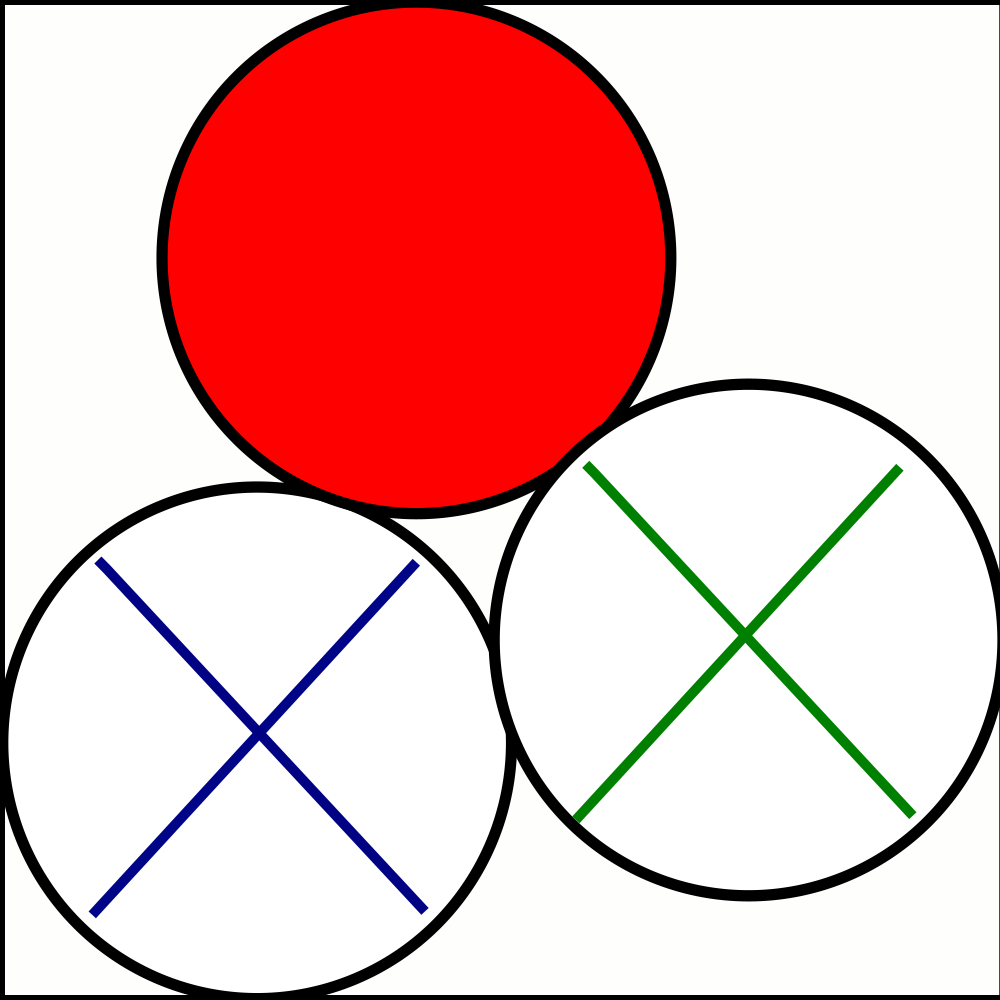
\includegraphics[width=0.5\linewidth]{./pixelRED}
\caption{Pixel LED rosso acceso}
\label{fig:pixelRED}
\end{figure}

Invece, quando si deve formare un colore come il viola, determinato dalla tripletta RGB (1,0,1), entrambi i LED rosso e blu sono accesi al massimo della loro intensità, determinando quindi un segnale certamente superiore a quello del rosso da solo. Questo è il motivo per cui sono visibili quei picchi che \underline{non} corrispondono ai colori singoli RGB, bensì alle loro combinazioni (1,1,0), (0,1,1), (1,0,1) (Figura (\ref{fig:pixelRED+BLUE})).

\begin{figure}
\centering
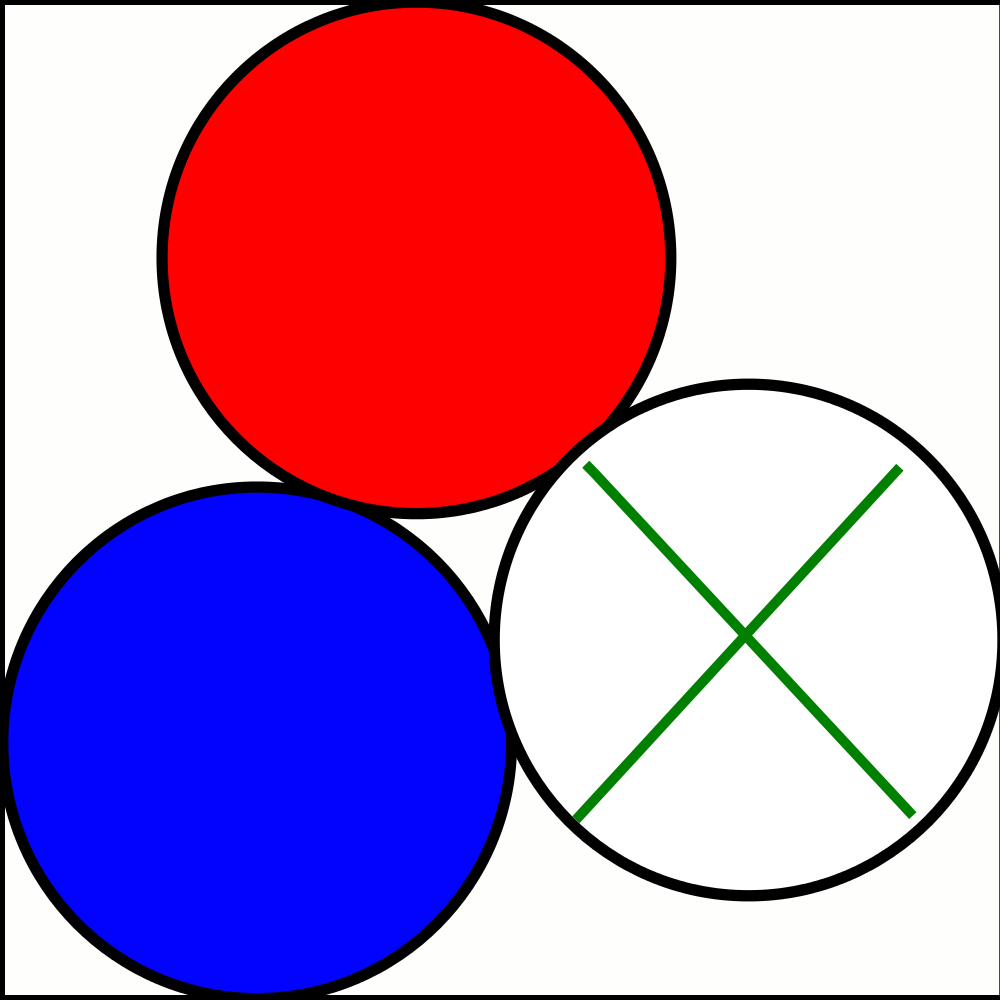
\includegraphics[width=0.5\linewidth]{./pixelRED+BLUE}
\caption{Pixel accesi blu+rosso}
\label{fig:pixelRED+BLUE}
\end{figure}

\begin{figure}
\centering
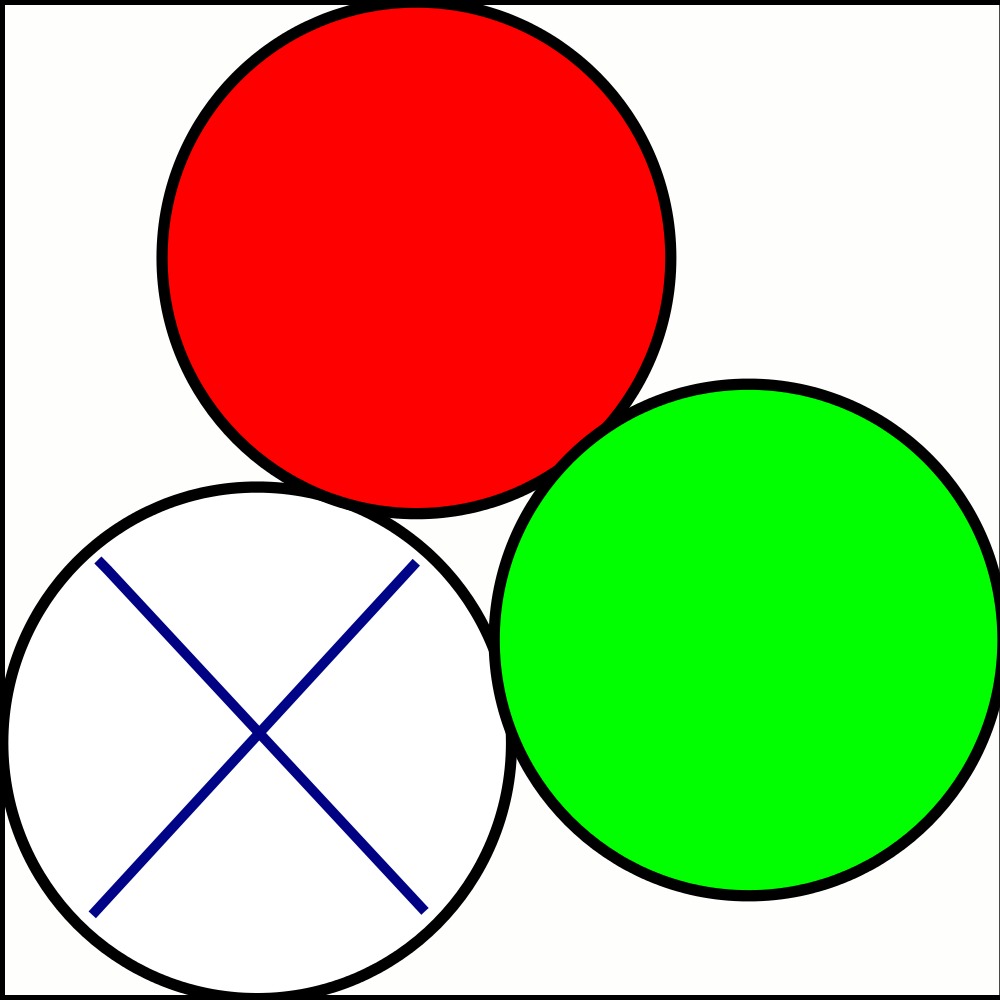
\includegraphics[width=0.5\linewidth]{./pixelRED+GREEN}
\caption{Pixel accesi rosso+blu}
\label{fig:pixelRED+GREEN}
\end{figure}

La nostra ipotesi di lavoro è che ci sia una corrispondenza lineare fra float RGB e intensità luminosa del corrispondente LED, e che (dato che si tratta di frequenze diverse fra loro) il segnale risultante $S_{TOT}$ possa essere dato dalla somma dei segnali dei singoli LED moltiplicati ognuno per il coefficiente float $a_i$ della tripletta. Per cui, in formula:

\begin{equation}\label{sig}
S_{TOT} = a_R S_R + a_B S_B + a_G S_G
\end{equation}

~\\
Fondamentale per tutte le considerazioni che verranno effettuate di seguito, è approssimare la relazione fra intensità (e quindi potenza) incidente sulla cella fotovoltaica con la tensione misurata ai suoi capi. Ovviamente, questo non è in generale vero, ma siamo incoraggiati dal risultato ottenuto in precedenza (vedi Figura (\ref{fig:es8_fit_tens})) per cui si verifica una relazione di tipo logaritmico fra tensione e potenza incidente. Dato che le tensioni misurate in questa parte dell'esperienza sono inferiori ai 20mV, ci troviamo nella regione del logaritmo prossima allo zero (x=1), dove questo può essere ben approssimato con una funzione lineare.\\

Se prendiamo come riferimento per il segnale rosso, verde e blu le "valli" dei picchi, riportiamo nel grafico in Figura (\ref{fig:color_300_modello_lin}) il segnale effettivamente acquisito (in nero) e quello simulato con il nostro modello (in verde).\\

\begin{figure}
\centering
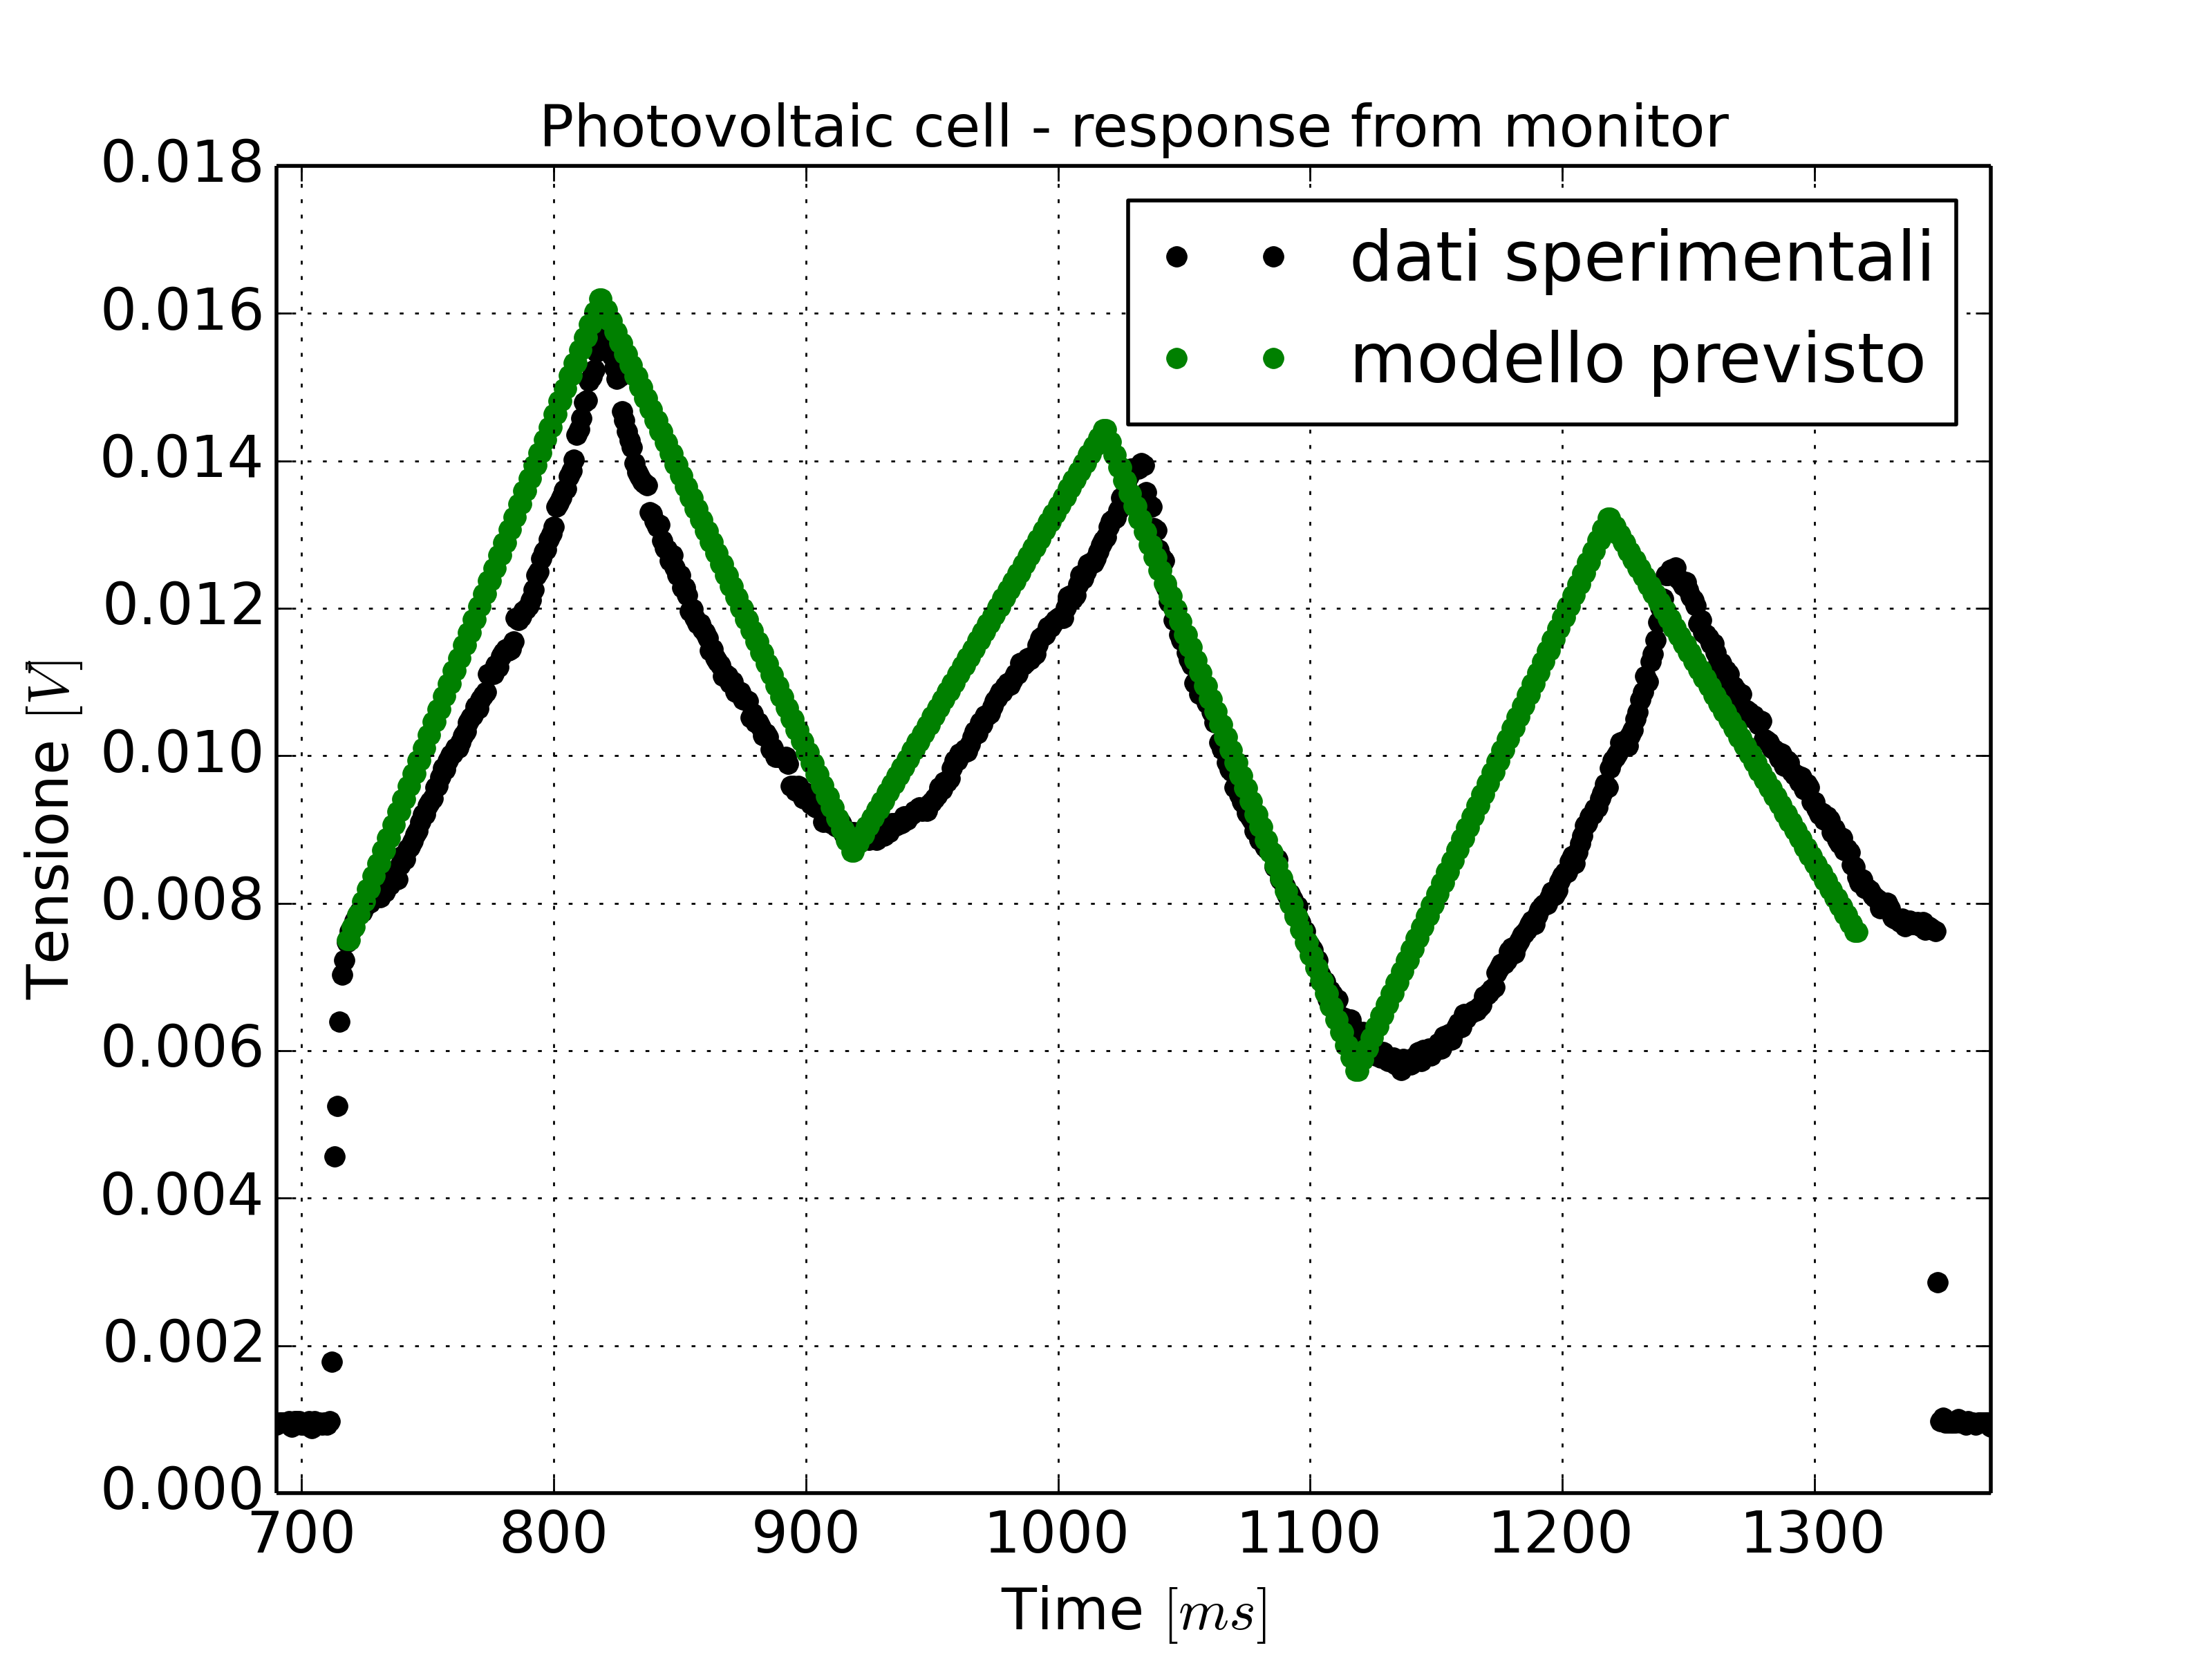
\includegraphics[width=0.9\linewidth]{./color_300_modello_lin}
\caption{Simulazione del segnale della cella in funzione del tempo - confronto dati sperimentali}
\label{fig:color_300_modello_lin}
\end{figure}

Notiamo una corrispondenza davvero notevole fra le due curve, il che potrebbe indicare che il nostro modello è abbastanza valido! Tuttavia, salta all'occhio un certo ritardo che aumenta linearmente al passare del tempo fra le curve, che porta ad uno "sfasamento" finale di 0.15 s (nella nostra scala dei tempi/campionamenti corrisponde a 30 samples). Tale sfasamento non era previsto, poichè la frequenza di campionamento è stata fissata tale da ottenere 2 rilevazioni per ogni tripletta RGB, per cui per 300 triplette, 600 punti sperimentali (ne risultano 630). Ciò potrebbe essere dovuto al fatto che la gestione del tempo di Octave non è ottimale, con un ritardo di circa 1ms per ogni aggiornamento del colore.\\
Per ovviare a questo inconveniente, è stata fatta una opportuna "dilatazione" del modello, in modo da procedere con l'analisi dei dati (Figura (\ref{fig:3_315_modello_lin})). \\

\begin{figure}
\centering
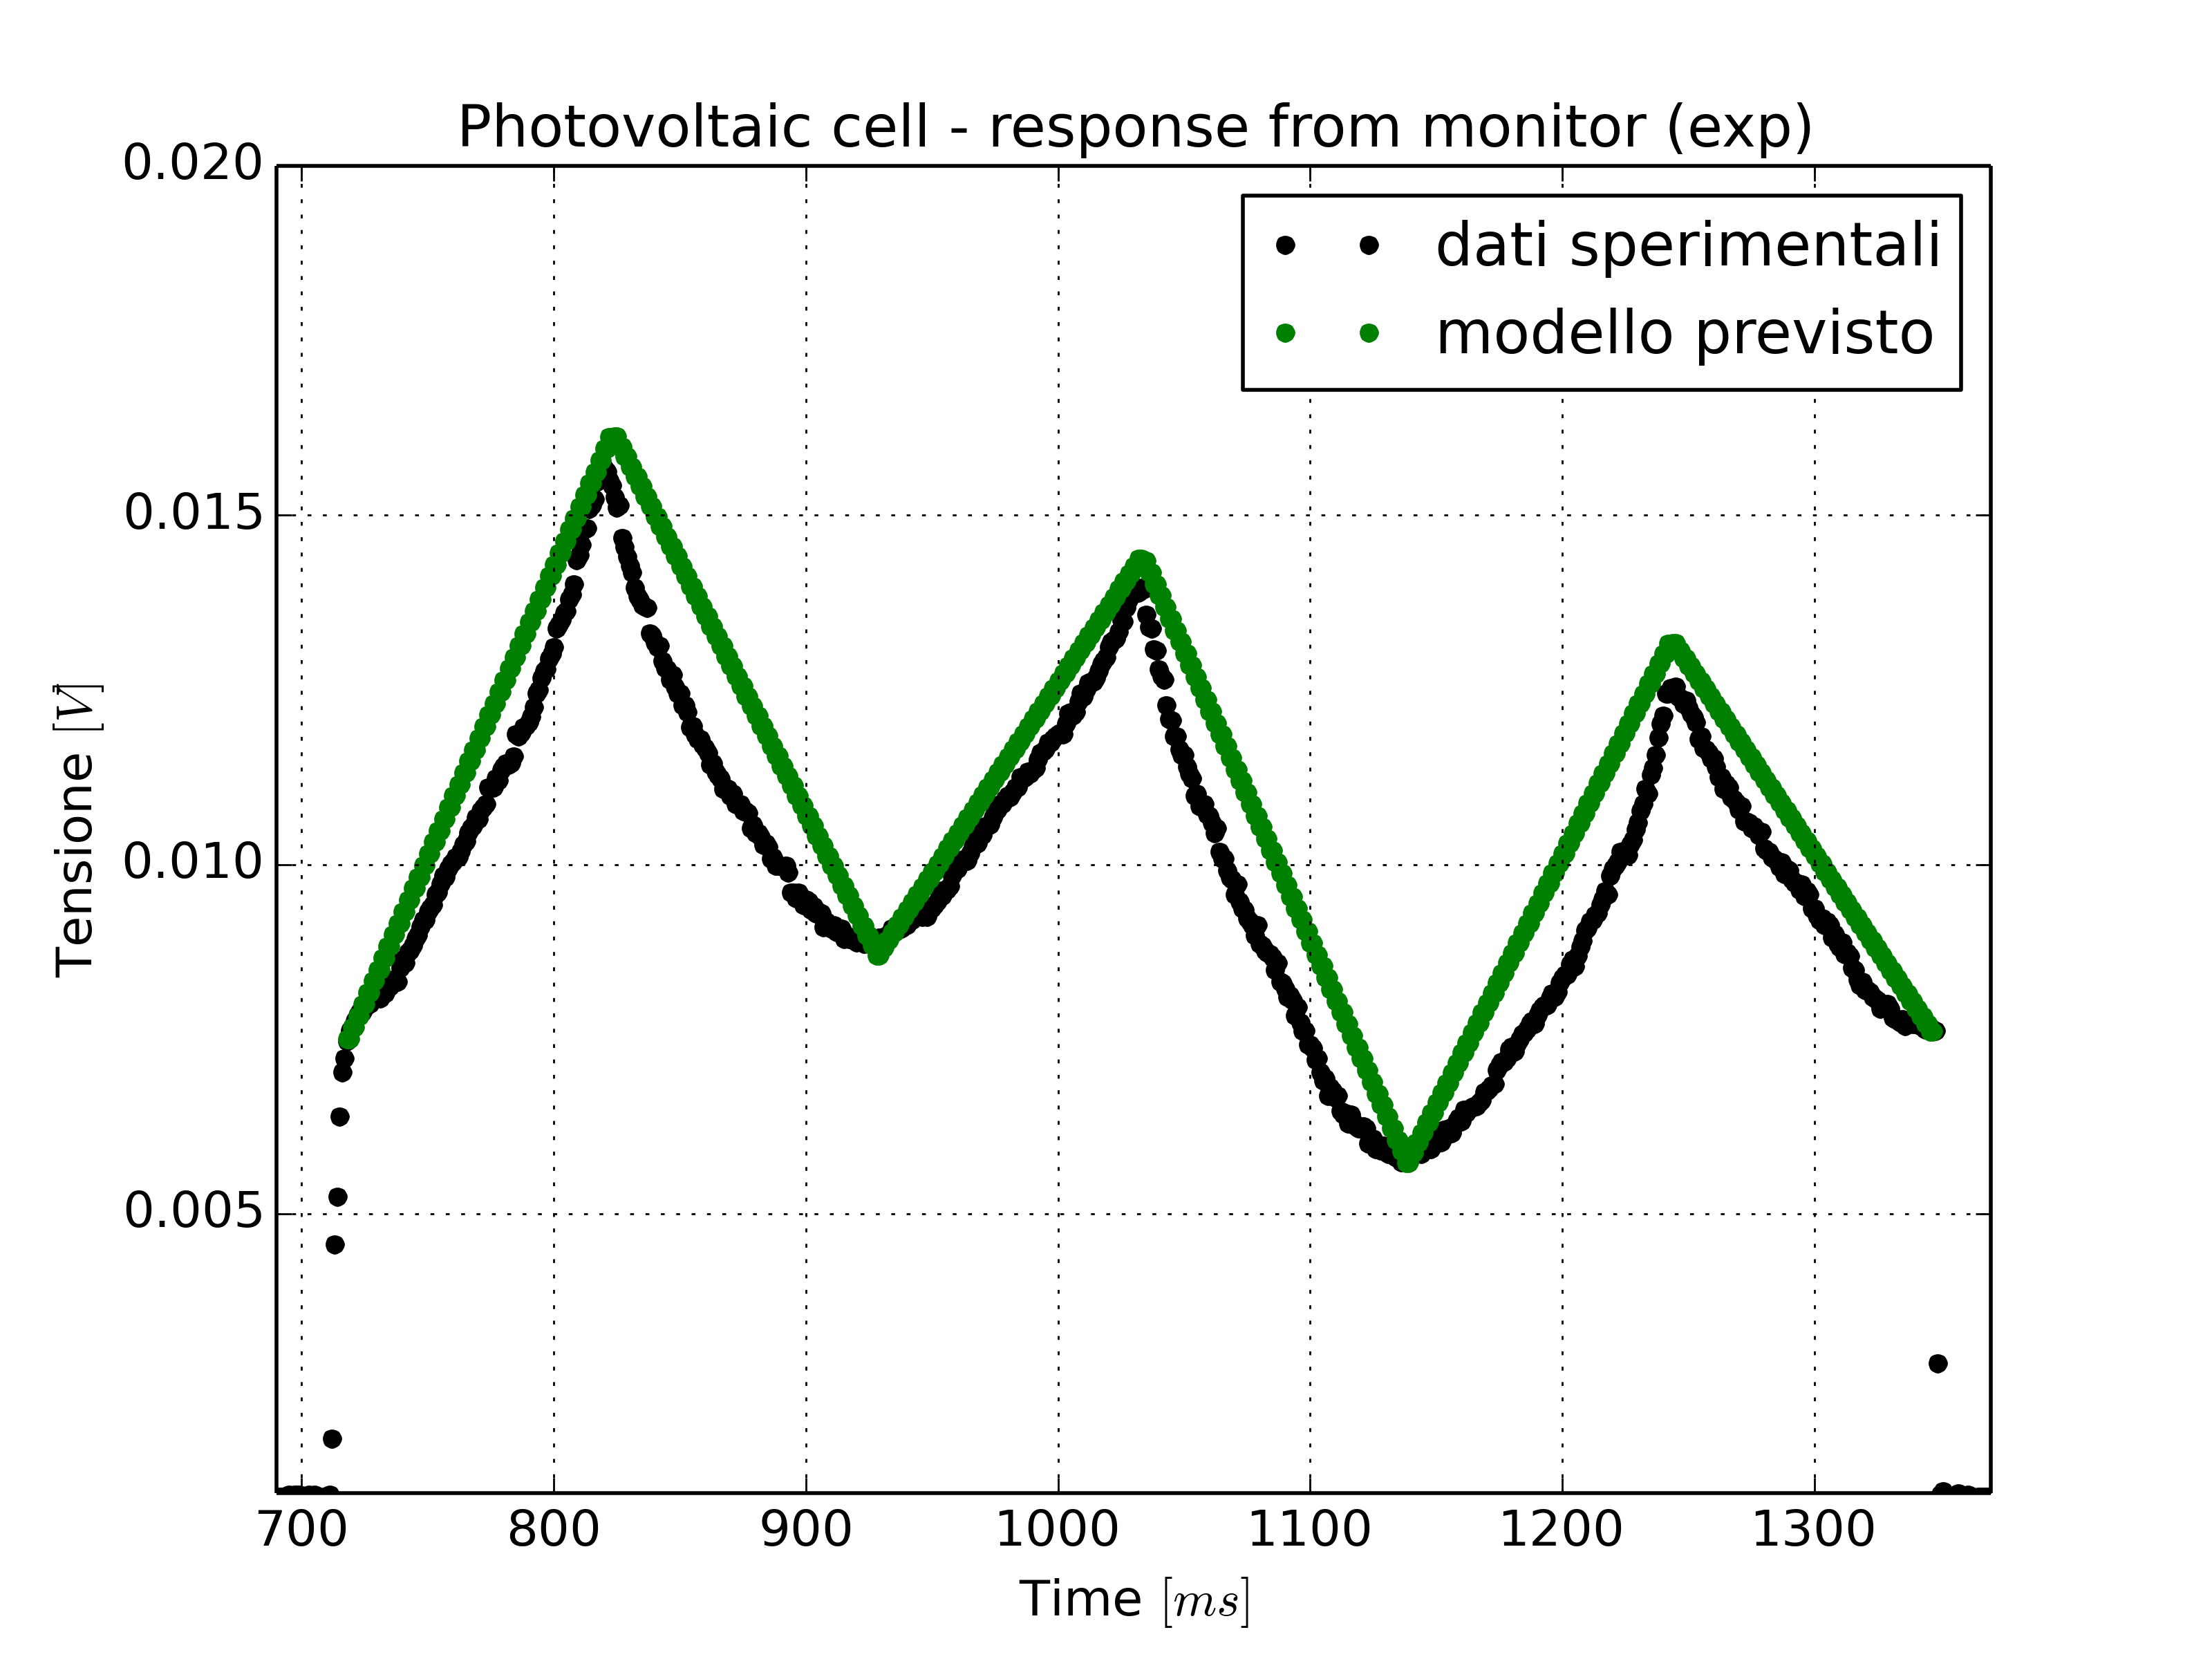
\includegraphics[width=0.8\linewidth]{./relaz_colori/3_315_modello_lin}
\caption{Modello lineare (dilatato) e dati sperimentali}
\label{fig:3_315_modello_lin}
\end{figure}


A partire dalla (\ref{sig}), risulta naturale normalizzare il segnale "complessivo" in modo da tener conto della potenza aggiuntiva data dal LED in più acceso in tutte le combinazioni (1,x,0) come segue:

\begin{equation}\label{sig_norm}
S_{TOT} = \frac{a_R S_R + a_B S_B + a_G S_G}{a_R + a_B + a_G}
\end{equation}

In Figura (\ref{fig:4_315_modello_lin+mod_norm}) è riportato lo stesso grafico di prima con il modello normalizzato. In Figura (\ref{fig:5_315_modello_lin_mod_norm_datanorm}), invece, procediamo a normalizzare anche i dati effettivamente acquisiti, dividendo il segnale per la somma dei coefficienti della tripletta corrispondente al colore generato.\\
Come ci si aspetta, l'accordo è buono.\\

\begin{figure}
\centering
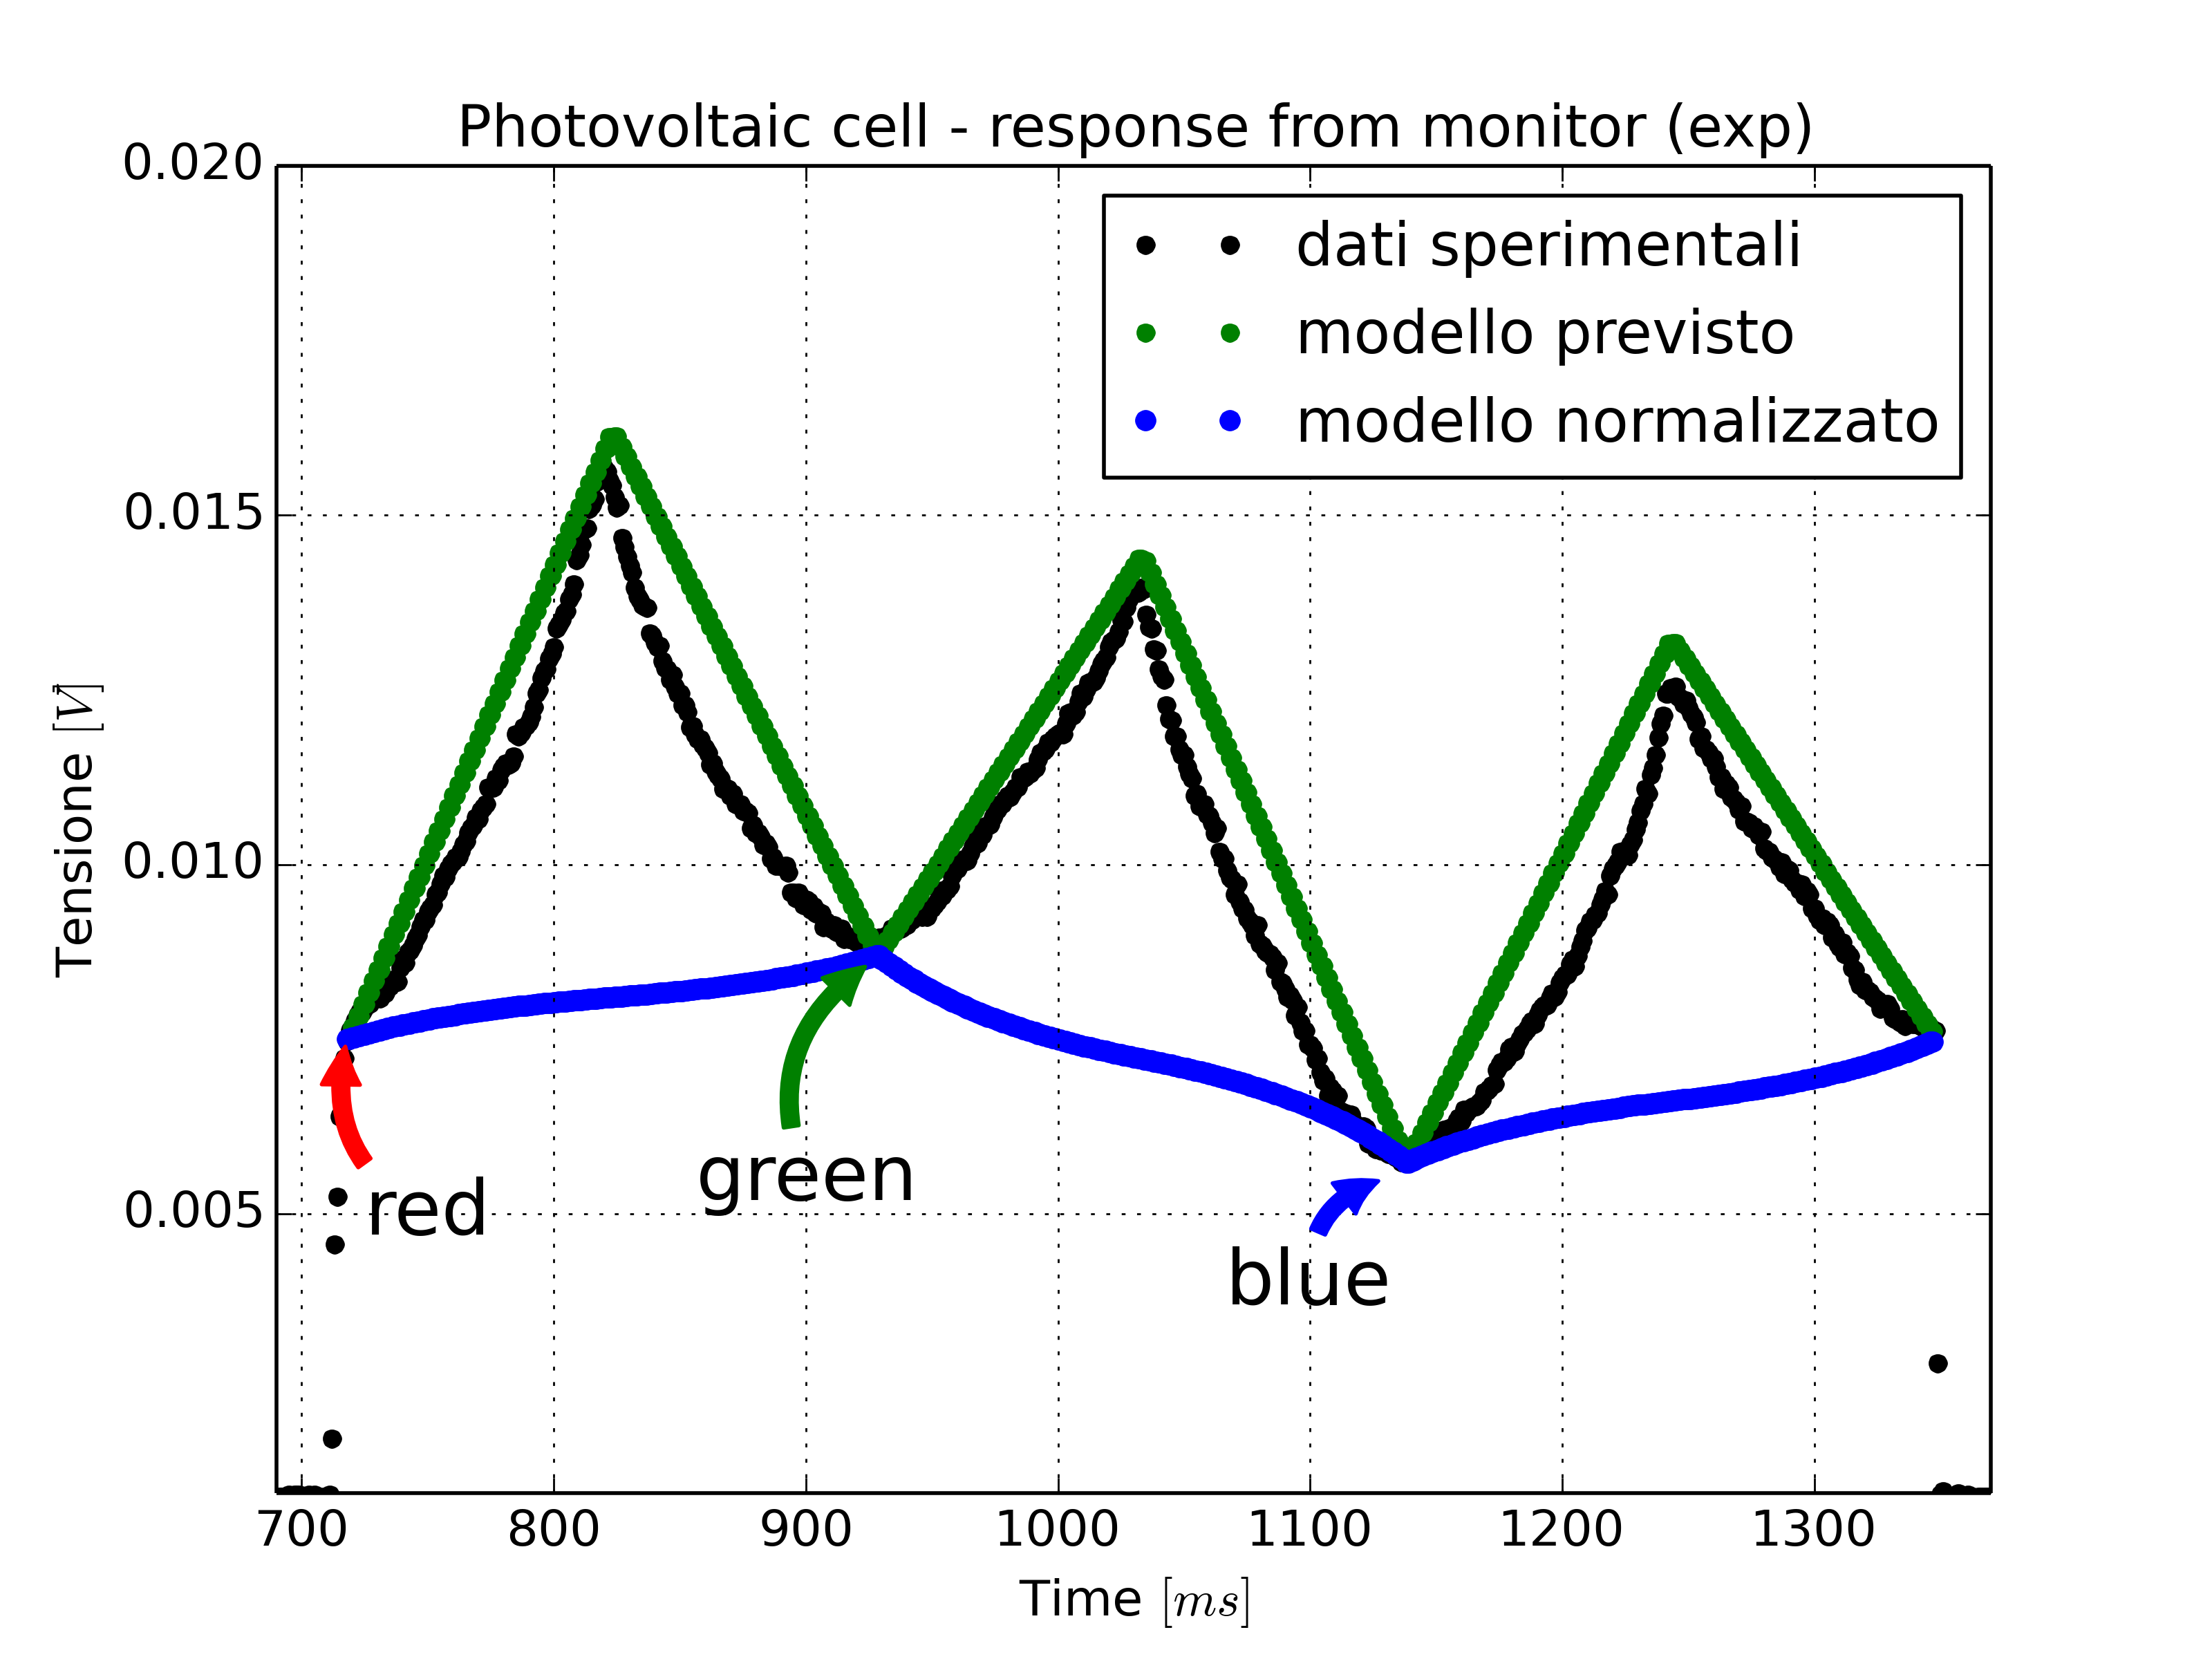
\includegraphics[width=0.8\linewidth]{./relaz_colori/4_315_modello_lin+mod_norm}
\caption{Modello lineare norm e dati sperimentali}
\label{fig:4_315_modello_lin+mod_norm}
\end{figure}


\begin{figure}
\centering
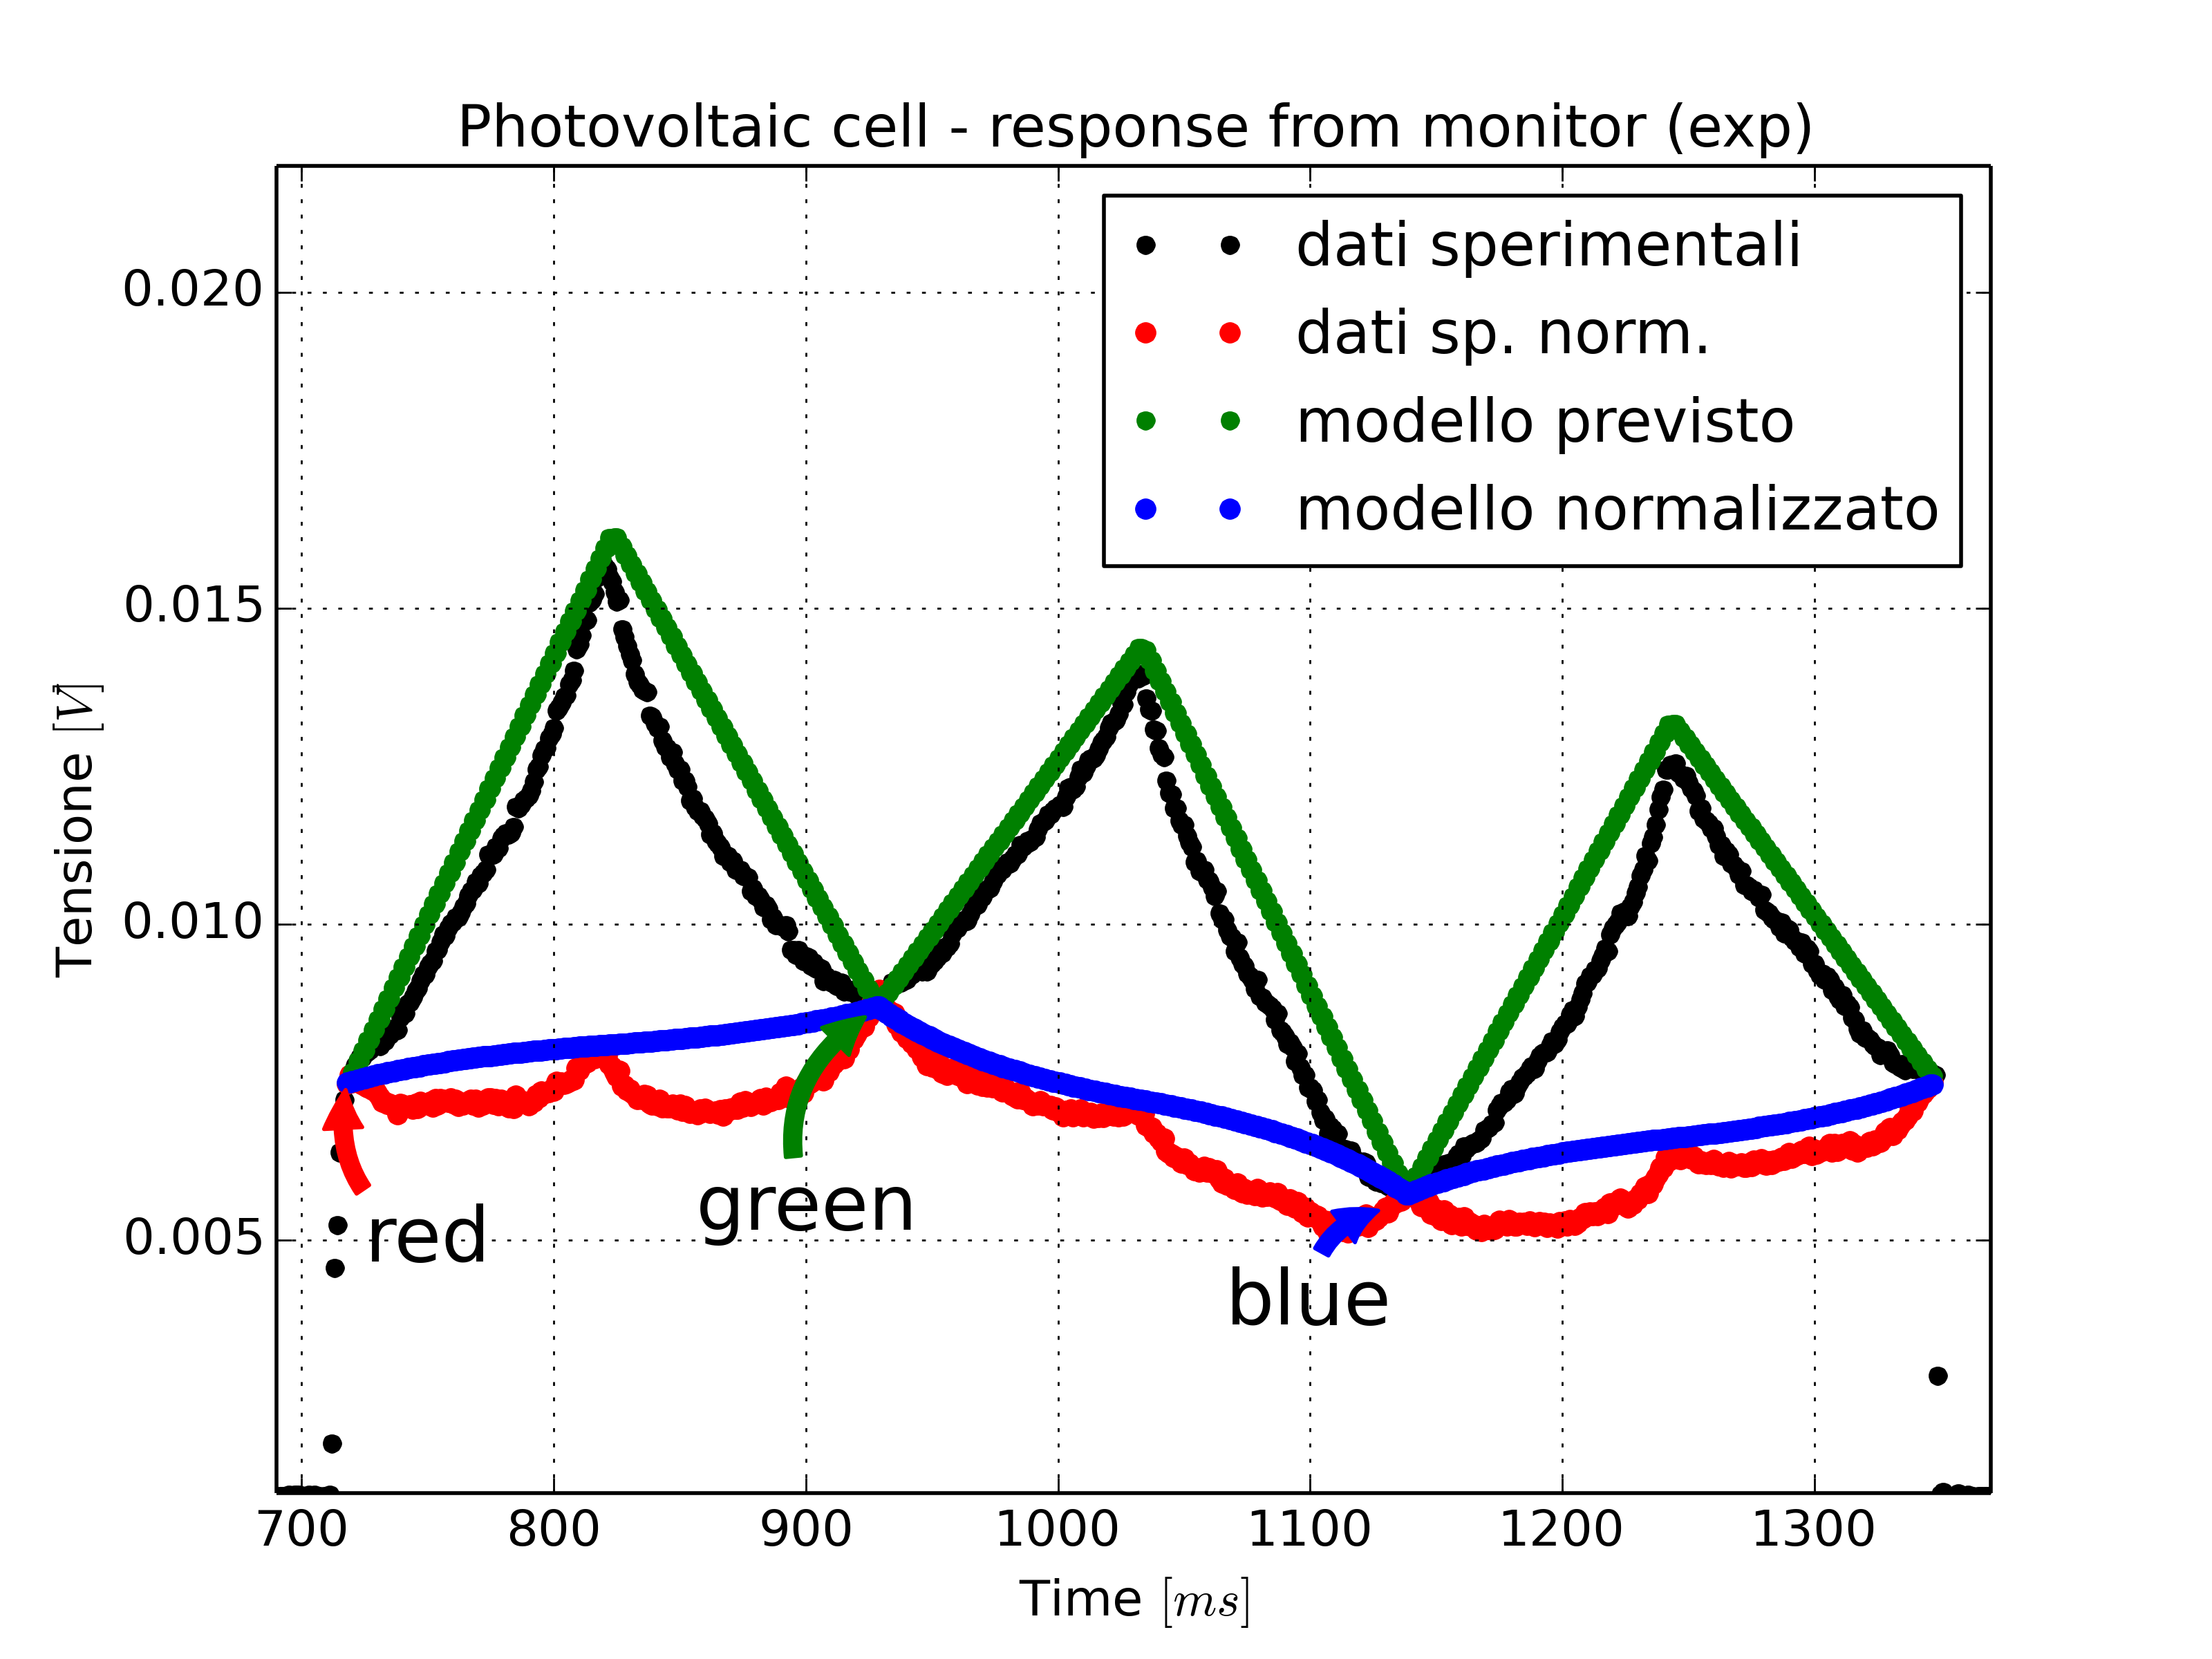
\includegraphics[width=0.8\linewidth]{./relaz_colori/5_315_modello_lin_mod_norm_datanorm}
\caption{Modello lineare e dati sperimentali normalizzati}
\label{fig:5_315_modello_lin_mod_norm_datanorm}
\end{figure}


A questo punto, possiamo fare un passo successivo e provare a verificare un'ulteriore ipotesi, e cioè che l'intensità del LED sia una combinazione lineare dei "segnali" RGB, ma con i \textbf{quadrati} dei coefficienti della tripletta. In formula:

\begin{equation}\label{sig_quad}
S_{TOT} = a_R^2 S_R + a_B^2 S_B + a_G^2 S_G
\end{equation}

Il motivo per cui studiamo questa ipotesi è che nelle fasi di risalita della tensione (che corrispondono a quelle triplette (1,x,0) con x che aumenta linearmente da 0 a 1) l'andamento sembra essere in realtà più simile ad una funzione quadratica che ad una lineare, data la concavità caratteristica di ogni salita/discesa. Proviamo, quindi, è simulare un modello quadratico e a sovrapporlo ai dati sperimentali, si veda Figura(\ref{fig:6_315_quadr}).

\begin{figure}
\centering
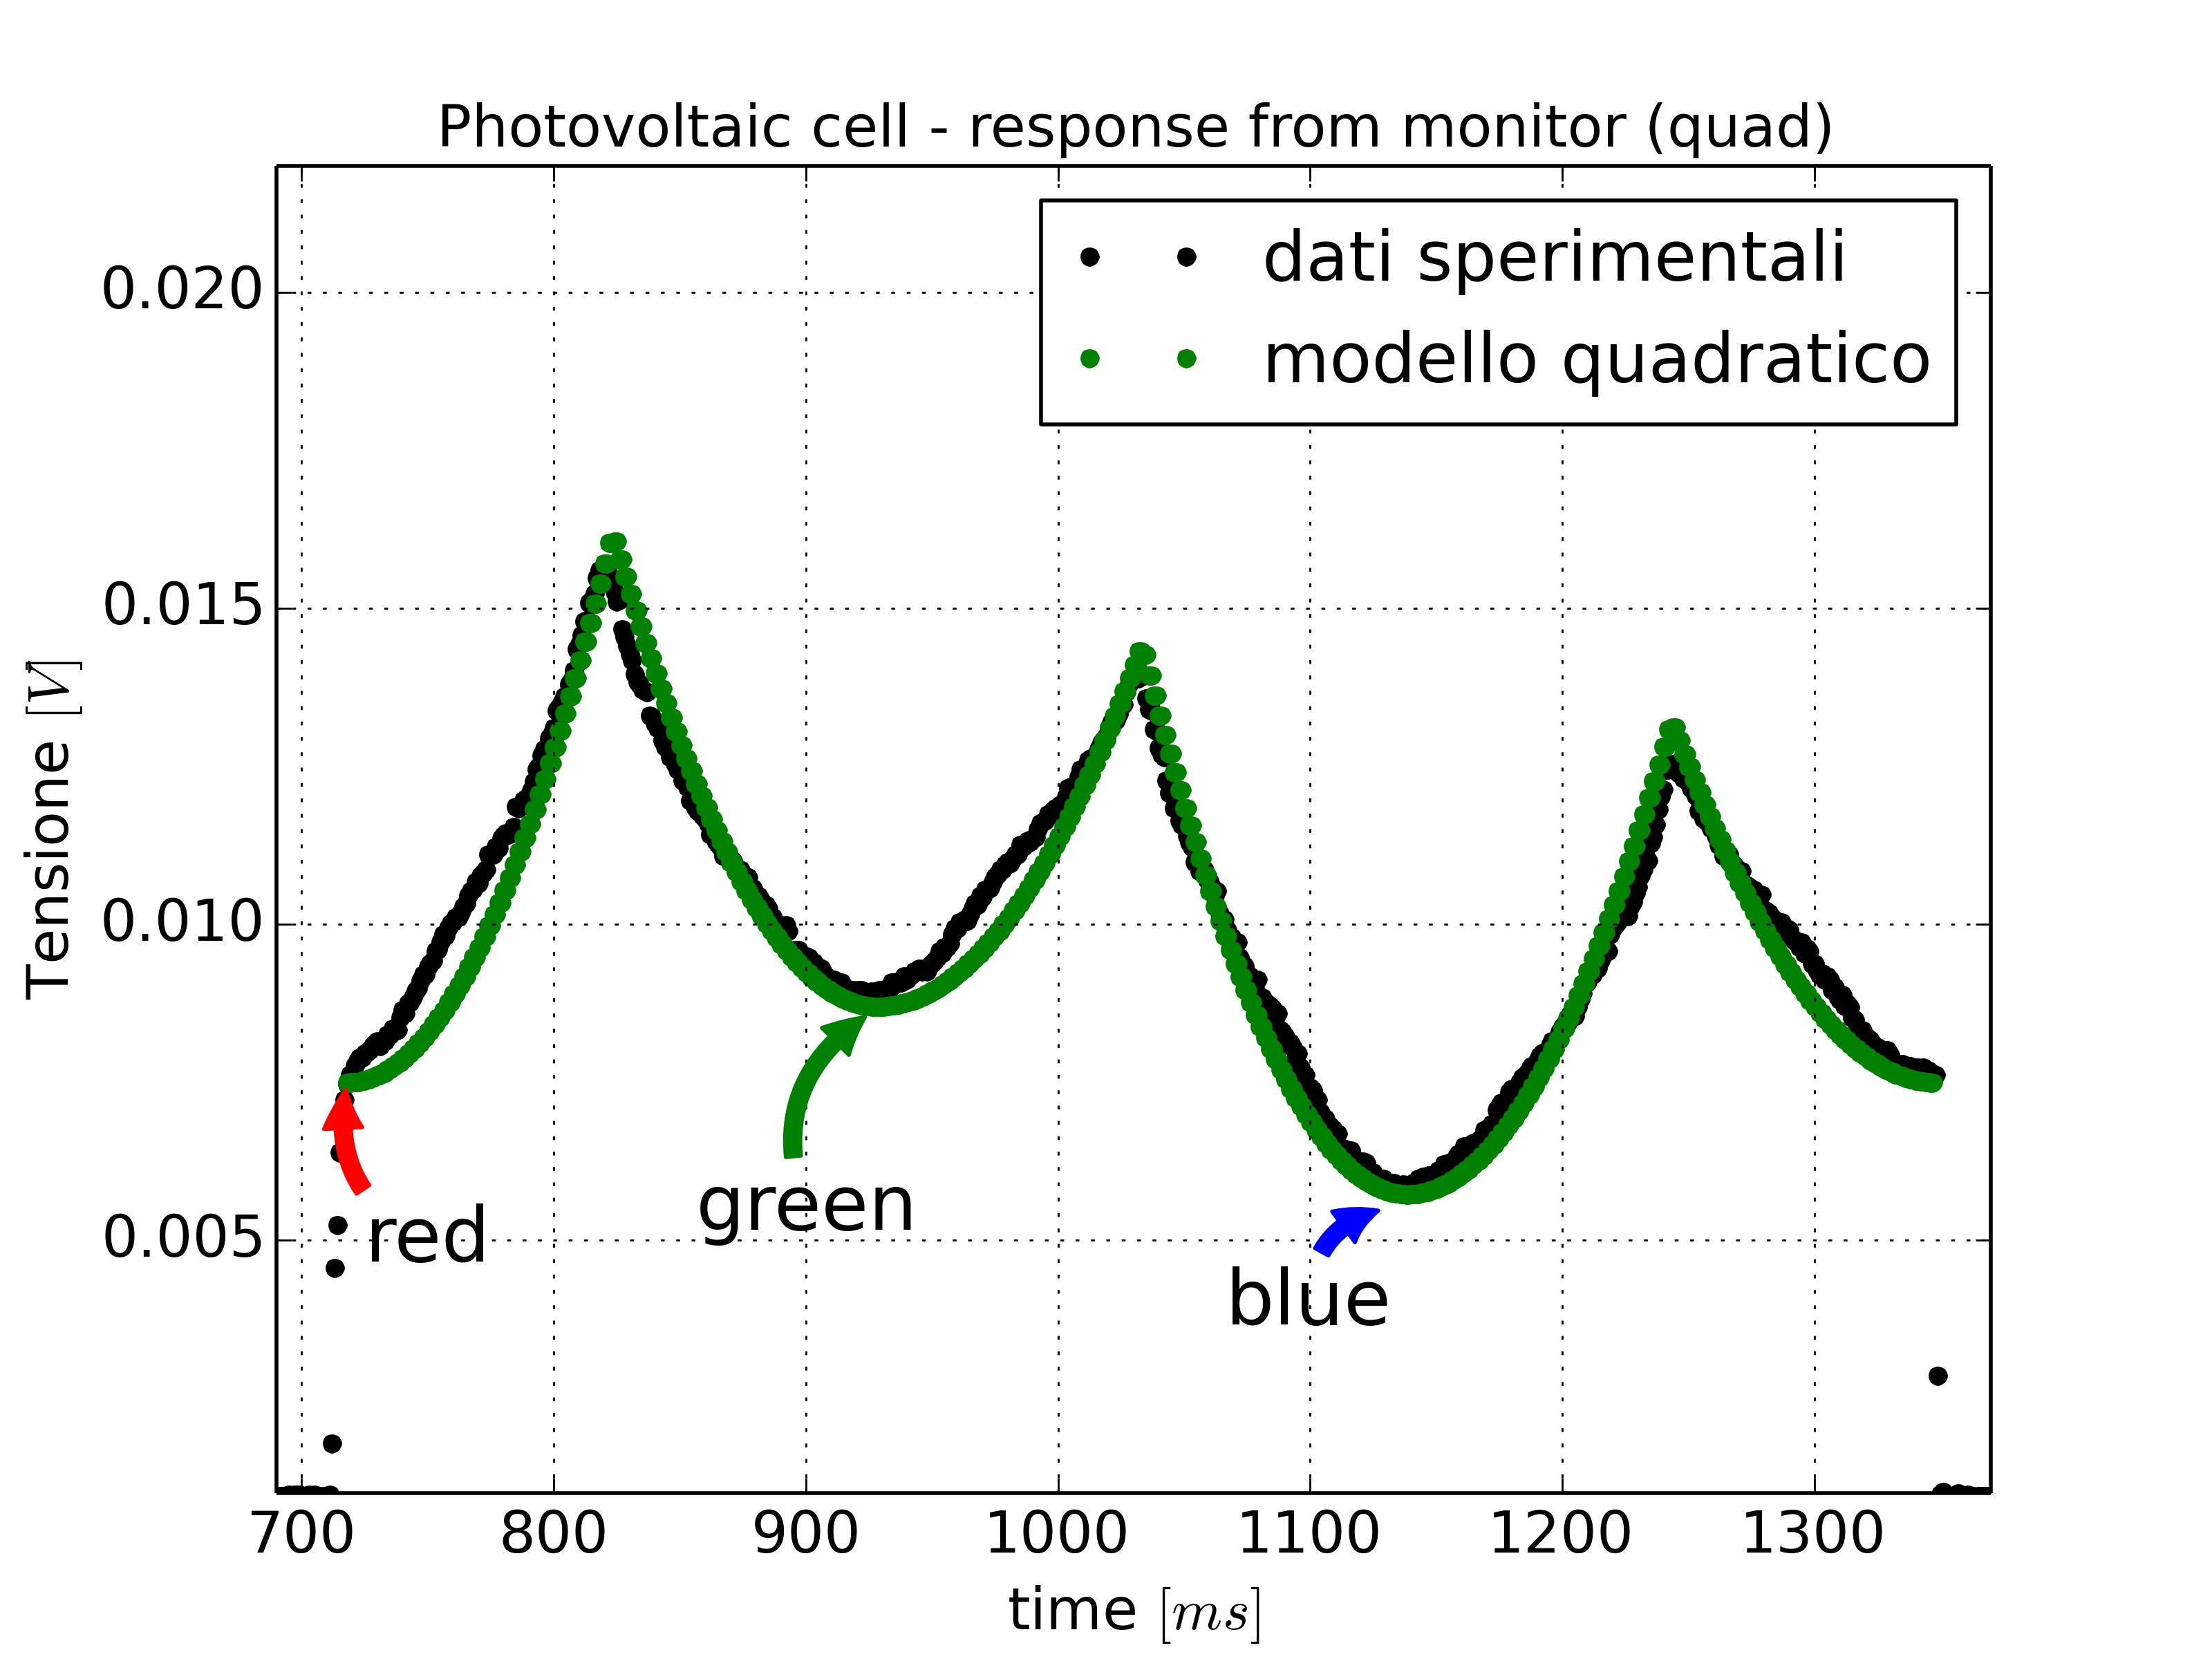
\includegraphics[width=0.8\linewidth]{./relaz_colori/6_315_quadr}
\caption{Modello quadratico e dati sperimentali.}
\label{fig:6_315_quadr}
\end{figure}



Il risultato è davvero notevole: le due curve sono quasi sovrapposte per la maggior parte della durata dell'acquisizione. Come ulteriore \textit{check}, normalizziamo entrambe le serie di dati secondo la:

\begin{equation}
S_{TOT} = \frac{a_R^2 S_R + a_B^2 S_B + a_G^2 S_G}{a_R^2 + a_B^2 + a_G^2}
\end{equation}

L'accordo fra le due serie normalizzate (Figura (\ref{fig:7_315_quadr_dati+modello})) è ancora migliore di quanto previsto dal modello lineare. Ovviamente, per avereuna conferma definitiva della validità di un modello rispetto all'altro, bisogna trovare la relazione esatta che (costruttivamente e a livello di software) lega i valori RGB all'intensità dei LED che potrebbero essere comandati in corrente, tensione...

\begin{figure}
\centering
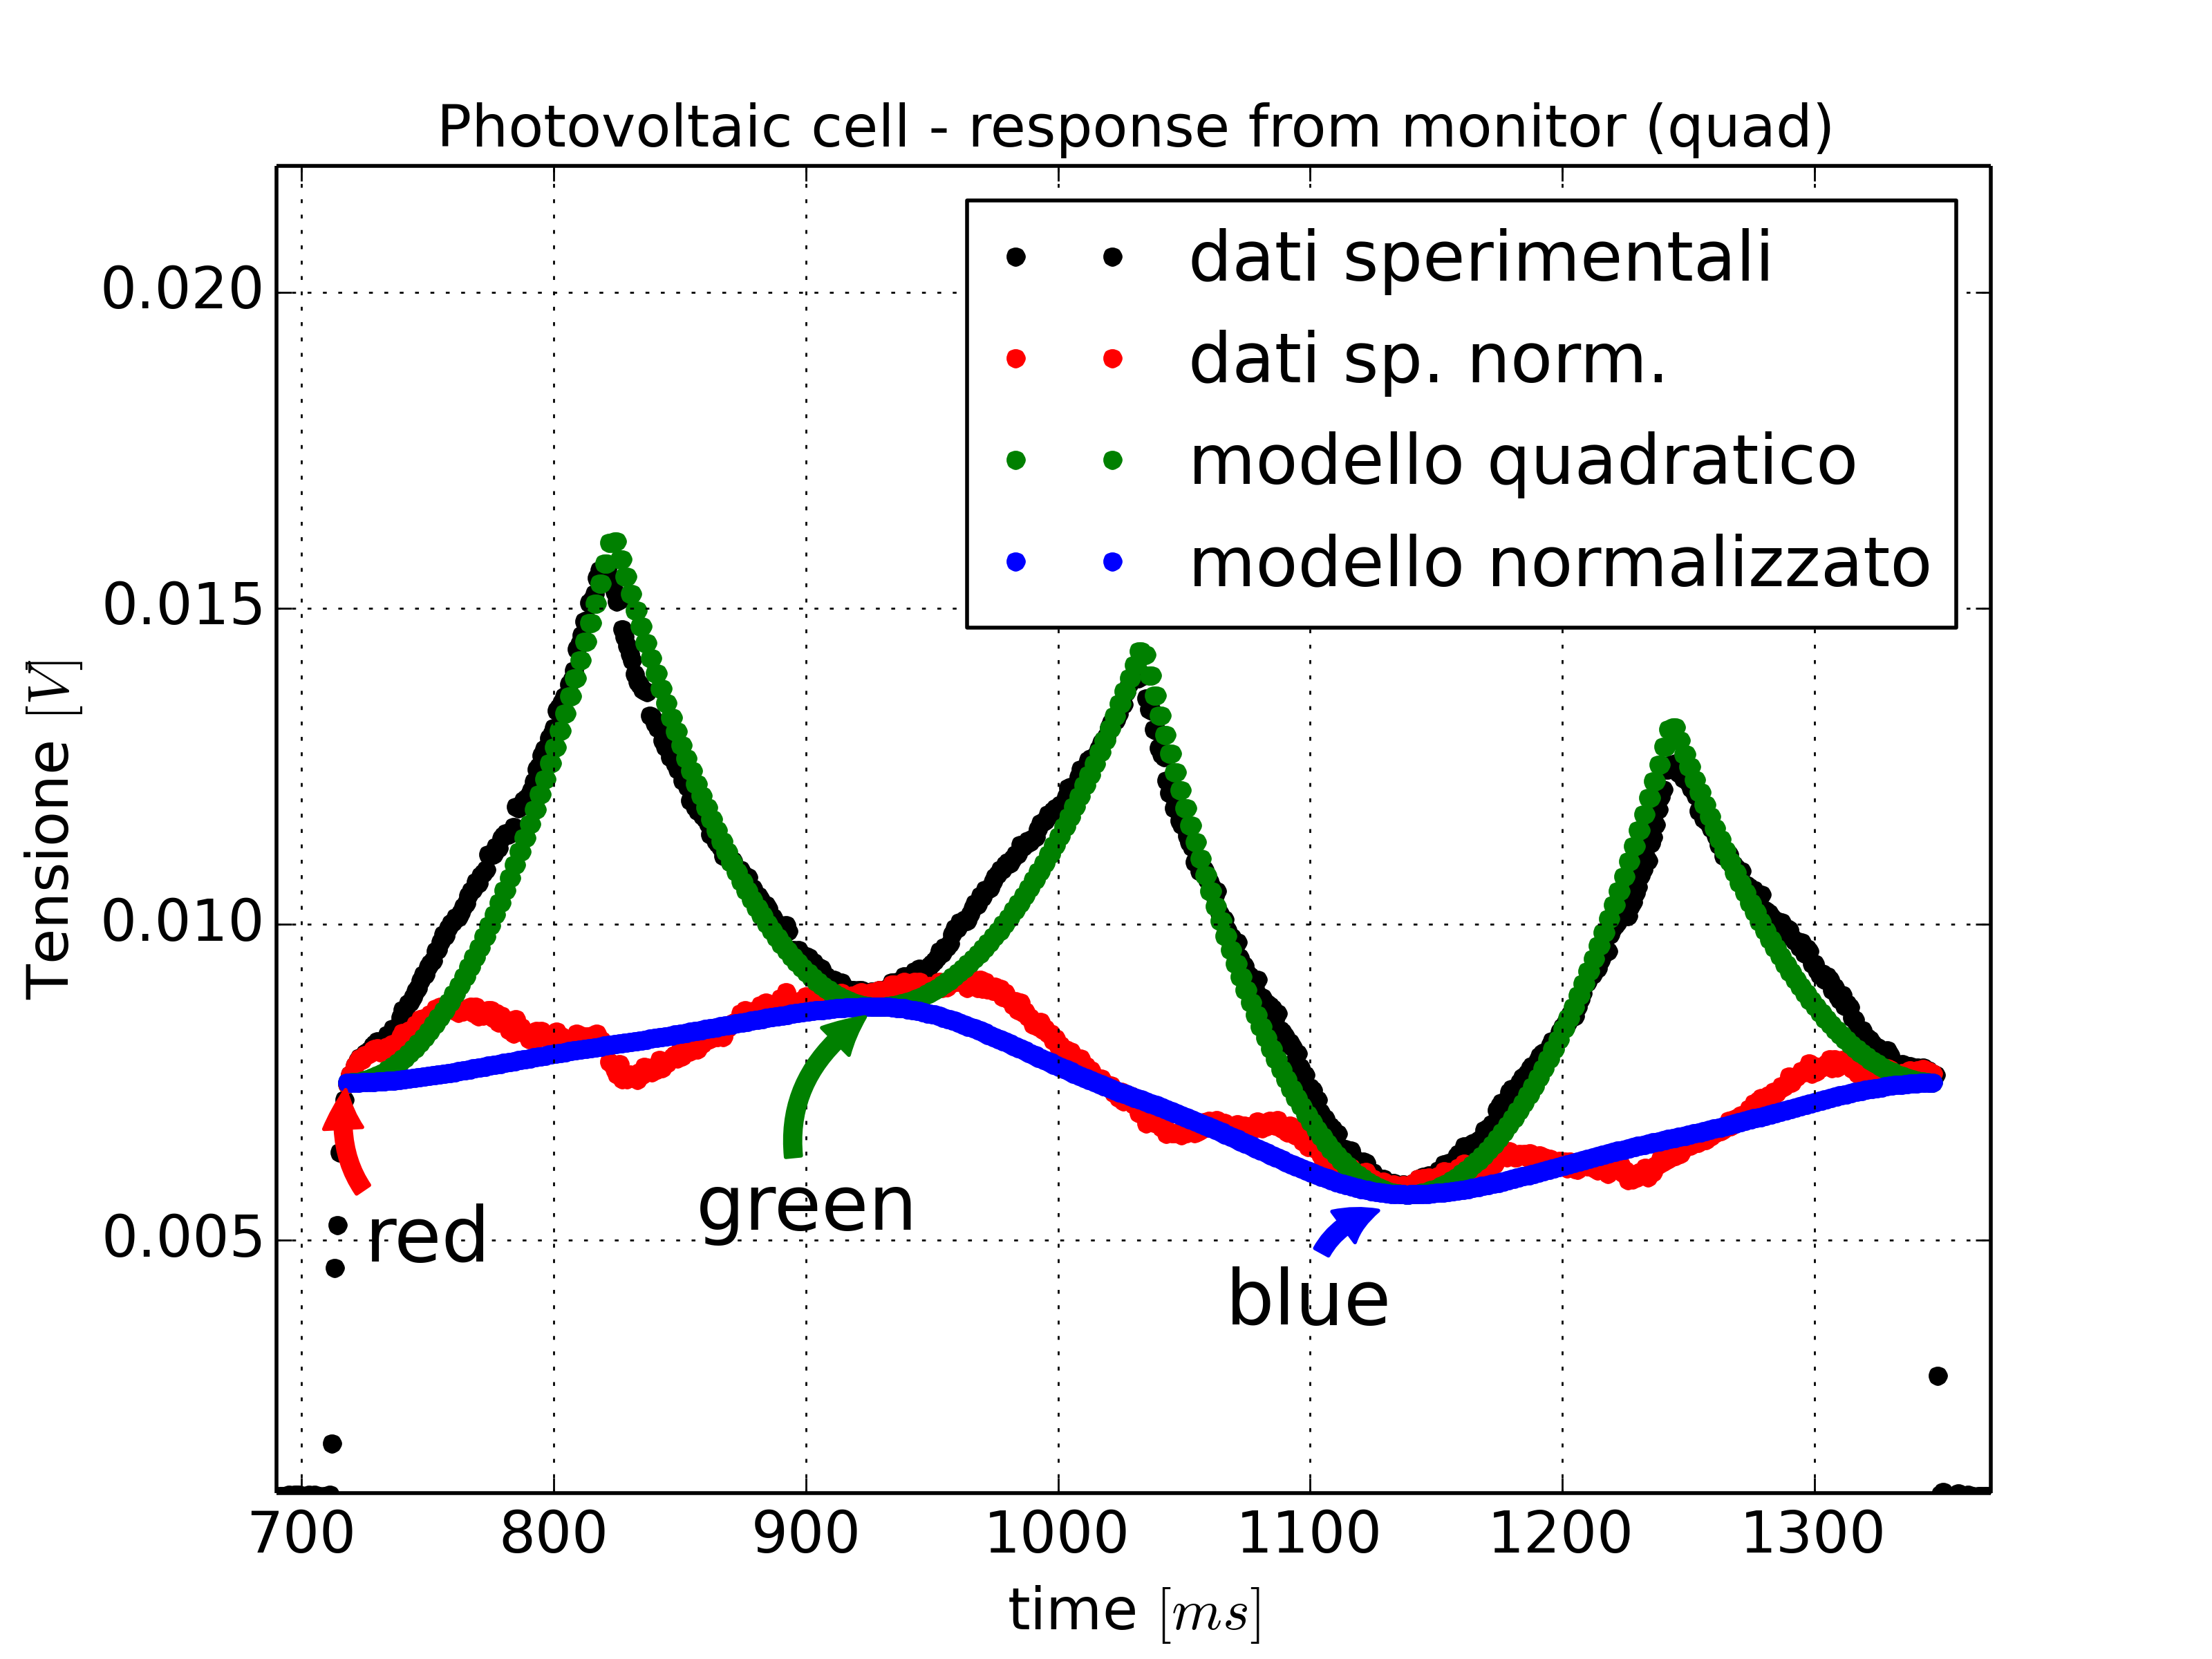
\includegraphics[width=0.8\linewidth]{./relaz_colori/7_315_quadr_dati+modello}
\caption{Modello quadratico e dati sperimentali normalizzati}
\label{fig:7_315_quadr_dati+modello}
\end{figure}


\section{Conclusioni}

L'obiettivo originale di questo approfondimento era quallo di ricavare una relazione fra la tensione ai capi della cella e la curva di responsività della stessa, come riportata (ad esempio) in Figura (1). Tuttavia, procedendo con queste analisi e valutazioni, ci siamo resi conto che ciò non è possibile per una serie di motivi (alcuni costruttivi e altri proprio fisici):

\begin{itemize}
\item Lo standard RGB è stato scelto ed è ormai il più diffuso su tutti i monitor perchè è quello che permette una resa migliore dei colori appartenenti allo spettro del visibile, calibrati sulla proporzione fra i coni e i bastoncelli presenti sulla retina e a loro volta non equamente distribuiti in numero in base alla frequenza incidente; ma fisicamente è ben diverso sovrapporre due o tre radiazioni di lunghezza d'onda \textbf{fissata} e di intensità variabile o invece emetterne una sola. 

\item Inoltre, proprio per questioni di resa cromatica, è nota la commercializzazione di monitor in cui la superficie occupata dai LED blu è in proporzione maggiore rispetto a quella dei LED RG, così come la loro intensità relativa è decisamente arbitraria.

\item Infine, non tutti i colori dello spettro del visibile sono ottenibili combinando luce RGB. Si veda infatti in Figura (\ref{fig:8_CIExy1931_sRGB_gamut_D65}) dove è riportato un diagramma delle cromaticità (la figura curva) che rappresenta i colori percepibili dall'occhio umano, con al suo interno lo spazio dei colori ottenibili con triplette RGB (il triangolo), detto anche \textit{gamut}.

\item Soltanto i colori "semplici" rosso, verde e blu sono posti vicino a lunghezze d'onda ben definite dello spettro visibile, per questo motivo sarebbe assolutamente privo di senso cercare di "sovrapporre" il grafico della responsività sui dati acquisiti. Per curiosità, abbiamo comunque estrapolato i rapporti relativi fra le intensità dei colori "semplici", che potrebbero indicativamente corrispondere alle lunghezze d'onda di 600nm (rosso), 550nm (verde) e 470nm(blu). Il colore di riferimento è il verde, dato che corrisponde al segnale di modulo maggiore.\\


\begin{tabular}{|c|c|}
\hline Colore RGB & Intens. relat. (to G) \\ 
\hline GREEN & 1 \\ 
\hline RED & 0.854 \\ 
\hline BLUE & 0.663 \\ 
\hline 
\end{tabular} 
\end{itemize}
~\\

Per tutti questi motivi, possiamo escludere di trarre informazioni riguardo la responsività spettrale della nostra cella, tuttavia abbiamo comunque realizzato un modello capace di spiegare (per un dato schermo e impostazioni fisse) i risultati del nostro esperimento in maniera più che soddisfacente, con valore predittivo.

\begin{figure}
\centering
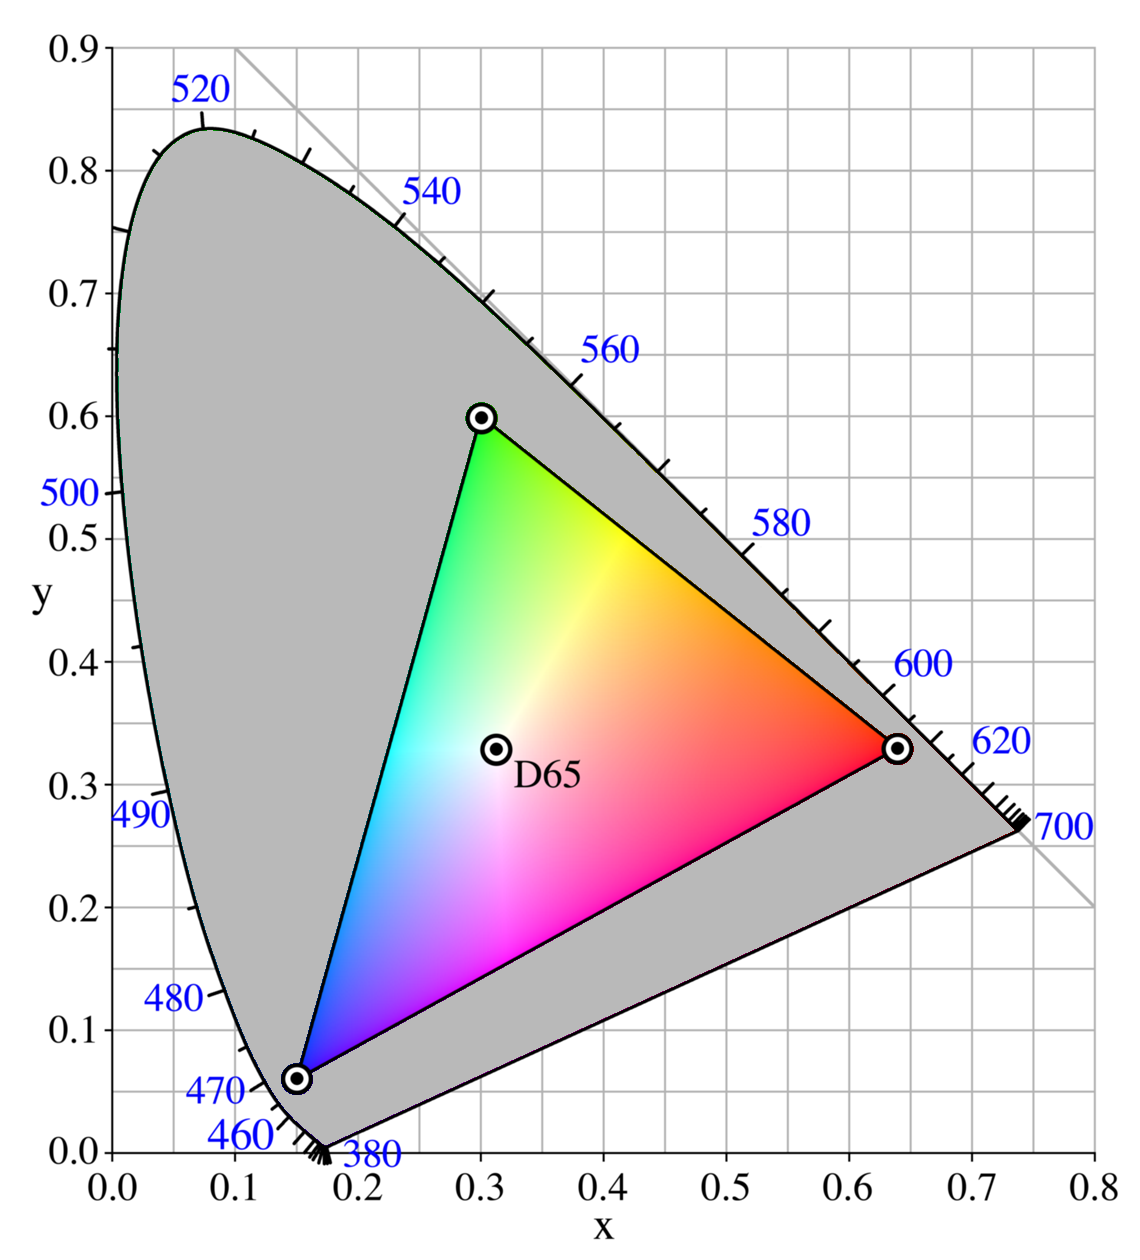
\includegraphics[width=0.8\linewidth]{./relaz_colori/8_CIExy1931_sRGB_gamut_D65}
\caption{Diagramma della cromaticità}
\label{fig:8_CIExy1931_sRGB_gamut_D65}
\end{figure}



\begin{thebibliography}{5}

	%Each item starts with a \bibitem{reference} command and the details thereafter.
	\bibitem{HOP96} % Transaction paper
	Datasheet, $\mu $A741 General-Purpose Operational Amplifiers. SLOS094E – NOVEMBER 1970  –REVISED JANUARY 2015.
	\url{http://www.ti.com/lit/ds/symlink/ua741.pdf}

	\bibitem{MJ06} % Conference paper
	Product data sheet: 1N4148 High-speed diodes. NXP Semiconductors 2004 Aug 10.
	\url{http://www.nxp.com/documents/data_sheet/1N4148_1N4448.pdf}

	\bibitem{MJH0} % Conference paper
	Product data sheet: AD711 op-amp.
	\url{http://www.analog.com/media/en/technical-documentation/data-sheets/AD711.pdf}
	
	\bibitem{JH06} % Conference paper
	Product data sheet: OP27 op-amp.
	\url{http://www.analog.com/media/en/technical-documentation/data-sheets/OP27.pdf}
	
	\bibitem{JH6} % Conference paper
	Product data sheet: tl081 op-amp.
	\url{http://www.ti.com/lit/ds/symlink/tl081.pdf}

	\bibitem{M06} % Conference paper
	Paul Horowitz, Winfield Hill - The Art of Electronics. Cambridge University Press (1989).
	
\end{thebibliography}

\end{document}